% tipo di documento
\documentclass[a4paper, twoside, openright]{report}
% codifica caratteri
\usepackage[utf8]{inputenc}
% encoding del testo
\usepackage[T1]{fontenc}
% dimensione dei margini
\usepackage[a4paper,top=2.5cm,bottom=2.5cm,left=3cm,right=3cm]{geometry}
% dimensione del font
\usepackage[fontsize=12pt]{scrextend}
% lingua del testo
\usepackage[english,italian]{babel}
% lingua per la bibliografia
\usepackage[fixlanguage]{babelbib}
% package per generare testo fittizio. Potrebbe essere
% utile nel controllare quanto un capitolo potrebbe essere
% grande e quindi quanto occupa nella pagina
\usepackage{lipsum}
% per ruotare le immagini
\usepackage{rotating}
% per modificare l'header delle pagine 
\usepackage{fancyhdr}
% per allineare in modo giustificato
\usepackage{ragged2e}
\justifying
% uso delle immagini
\usepackage{graphicx}
\usepackage{float}
% uso dei colori
\usepackage[dvipsnames, table]{xcolor}         
% uso dei listing per il codice
\usepackage{listings}          
% per inserire gli hyperlinks tra i vari elementi del testo 
\usepackage[colorlinks=true, allcolors=black]{hyperref}    
% diversi tipi di sottolineature
\usepackage[normalem]{ulem}
% package e comando per creare pagine vuote
\usepackage{afterpage}
\newcommand\blankpage{%
    \null
    \thispagestyle{empty}%
    \addtocounter{page}{-1}%
    \newpage
}
    
% package per creare comandi personalizzati
\usepackage{xpatch}
% package helper per le liste puntate
\usepackage{enumitem}
% package per l'utilizzo dei colori
% package per l'highlighting del codice
\usepackage{minted}
% package per gestire le caption
\usepackage{caption}
\usepackage{subcaption}
% per gestire tabelle su più pagine
\usepackage{longtable}
% per combinare le righe di una tabella
\usepackage{multirow}
% per creare i tree di directory
\usepackage{dirtree}

% per le icone a fianco dei titoli di sezione
\usepackage{etoolbox}
\newcommand{\icon}[1]{\includegraphics[height=12pt]{#1}}
\robustify{\icon}

% -----------------------------------------------------------------
\usepackage{todonotes}
\usepackage[normalem]{ulem}
\newcommand{\LP}[2]{{\color{gray}{\sout{#1}}\color{red}{#2}}\marginpar{\scalebox{1}{$\color{red}LP$}}\color{black}}
\newcommand{\LPx}[2]{\color{gray}\ #1\ \color{red}\  #2 \color{black}}
\newcommand{\LPtodo}[1]{\todo[color=white,linecolor=red,size=\tiny]{{\color{red}{LP: #1}}}}
% -----------------------------------------------------------------


% Modifica lo stile dell'header
\pagestyle{fancy}
\fancyhf{}
\lhead{\rightmark}
\rhead{\textbf{\thepage}}
\fancyfoot{}
\setlength{\headheight}{15pt}

% Rimuove il numero di pagina all'inizio dei capitoli
\fancypagestyle{plain}{
  \fancyfoot{}
  \fancyhead{}
  \renewcommand{\headrulewidth}{0pt}
}

% comandi per cambiare temporaneamente la lingua
% abstract in inglese, al fine di cambiarne il titolo
\xpretocmd{\abstract}{\selectlanguage{english}}{}{} 
\xapptocmd{\endabstract}{\selectlanguage{italian}}{}{}

% formattazione e highlight del codice
\usemintedstyle{manni}
\setminted[typescript]{
    framesep=2mm,
    baselinestretch=1.2,
    fontsize=\ttfamily\footnotesize,
    linenos
}
% Stesso stile del template, applicato ai linguaggi della tesi.
\setminted[python]{
    framesep=2mm,
    baselinestretch=1.2,
    fontsize=\ttfamily\footnotesize,
    linenos,
    breaklines
}
\setminted[sql]{
    framesep=2mm,
    baselinestretch=1.2,
    fontsize=\ttfamily\footnotesize,
    linenos,
    breaklines
}

% Le tabelle della tesi sono richiamate per numero nel testo.
\captionsetup[table]{labelformat=default}

% environment per impostare il codice in piu' pagine
\newenvironment{code}{\captionsetup{type=listing}}{}

\usepackage{amssymb}
% Integrazioni necessarie ai contenuti, senza importare il vecchio preambolo.
\usepackage{amsmath}
\usepackage{amsthm}
\usepackage{booktabs,tabularx,array}
% Stile locale alle tabelle; usa solo pacchetti gia presenti nel template.
\definecolor{ThesisTableHeader}{gray}{0.94}
\definecolor{ThesisTableRule}{gray}{0.35}
\newcommand{\thesisTableSetup}{%
  \renewcommand{\arraystretch}{1.20}%
  \setlength{\tabcolsep}{5pt}%
  \setlength{\heavyrulewidth}{0.7pt}%
  \setlength{\lightrulewidth}{0.35pt}%
  \arrayrulecolor{ThesisTableRule}%
}
\AtBeginEnvironment{table}{\thesisTableSetup}
\AtBeginEnvironment{table*}{\thesisTableSetup}
\newcommand{\tablehead}[1]{\textbf{\boldmath #1}}
\newcolumntype{Y}{>{\raggedright\arraybackslash}X}
\captionsetup[table]{font=small,labelfont=bf,skip=8pt}

\usepackage{tikz}
\usetikzlibrary{arrows.meta}
\usepackage[italian,noabbrev]{cleveref}
\crefname{listing}{listato}{listati}
\Crefname{listing}{Listato}{Listati}
\graphicspath{{images/}{figures/dataset/}{figures/models/}{figures/results/}}
\setlength{\emergencystretch}{2em}
\numberwithin{equation}{chapter}
% Indice sintetico; le sottosezioni rimangono nel testo.
\setcounter{tocdepth}{1}
   \theoremstyle{plain}% default
\newtheorem{thm}{Theorem}[section]
\newtheorem{lem}[thm]{Lemma}
\newtheorem{prop}[thm]{Proposition}
\newtheorem*{cor}{Corollary}
\newtheorem*{KL}{Klein’s Lemma}
  \theoremstyle{definition}
\newtheorem{defn}{Definition}[section]
\newtheorem{conj}{Conjecture}[section]
\newtheorem{exmp}{Example}[section]
\newtheorem{exercise}{Exercise}[section]
  \theoremstyle{remark}
\newtheorem*{rem}{Remark}
\newtheorem*{note}{Note}
\newtheorem{case}{Case}
% -----------------------------------------------------------------
\begin{document}

\begin{titlepage}

\begin{center}
    \textbf{\huge{Università degli Studi di Torino}}
    \vspace{2mm}
    \\ \LARGE{Dipartimento di informatica}
    \vspace{5mm}
    \\ 
\includegraphics[keepaspectratio=true,scale=0.4]{images/unito_logo.png}
    \vspace{5mm}
\end{center}

\begin{center}
    \LARGE{Tesi di Laurea Triennale in Informatica} 
\end{center}

\vspace{15mm}
\begin{center}
    % Dimensione leggermente ridotta per il titolo su più righe.
    \textbf{\LARGE{Classificazione ibrida classico-quantistica delle
    morfologie galattiche: confronto tra bottleneck classici
    e circuiti quantistici variazionali}}
\end{center}
\vspace{30mm}

\begin{minipage}[t]{0.47\textwidth}
	{\large{Relatore:}{\normalsize\vspace{3mm}
	\bf\\ \large{Prof. Luca Paolini} \normalsize\vspace{3mm}\bf}}
\end{minipage}
\hfill
\begin{minipage}[t]{0.47\textwidth}\raggedleft
	{\large{Candidato:}{\normalsize\vspace{3mm} \bf\\ \large{Michele Scandone}}}
    \\[2mm] {\normalsize Matricola 1096271}
\end{minipage}

\vspace{40 mm}
\hrulefill
\\ \centering{\large{ANNO ACCADEMICO 2025/2026}}

\end{titlepage}

% Citazione personale facoltativa: attivare dopo averla compilata.
% \thispagestyle{plain}

{
\raggedleft
\textit{A very cool quote!}
\\ - Author of the quote

}
\begin{abstract}
This thesis investigates hybrid classical--quantum transfer learning
for galaxy morphology classification. A balanced dataset of 5,628
SDSS images, labelled using Galaxy Zoo classifications, supports a
binary task distinguishing elliptical and spiral galaxies and a
three-class task that additionally includes systems labelled as mergers.
A frozen, ImageNet-pretrained ResNet18 provides a shared representation
for classical heads and hybrid heads with four or eight simulated qubits.
The main comparison pairs the trainable quantum head with a classical
bottleneck of the same dimension; a frozen-circuit variant assesses the
contribution of training the circuit parameters.

The evaluation comprises 640 runs across ten stratified holdout
repetitions and four training regimes: 100, 300, 900 images and the
complete training split. Nested training subsets and shared validation
and test sets support paired comparisons. Macro-F1, bootstrap confidence
intervals and Holm-adjusted tests are complemented by per-class analysis,
probabilistic metrics and computational costs.

On the full binary task, the models achieve a Macro-F1 close to 0.96,
with no statistically supported advantage for the quantum head over the
matched classical control. On the full three-class task, the quantum
head has a lower mean Macro-F1 by 0.73 and 1.67 percentage points with
four and eight qubits, respectively. Reduced-data regimes do not reveal
a quantum advantage under the adopted protocol, while simulation requires
substantially more training time. The study provides a reproducible
benchmark that distinguishes predictive performance from the added
value of the quantum component and identifies concrete directions for
further investigation. Its conclusions concern the tested architectures
and simulation conditions, not quantum machine learning in general.
\end{abstract}

\thispagestyle{plain}
\vspace*{\fill}
\textit{Dichiaro di essere responsabile del contenuto dell’elaborato che presento al fine del conseguimento del titolo, di non avere plagiato in tutto o in parte il lavoro prodotto da altri e di aver citato le fonti originali in modo congruente alle normative vigenti in materia di plagio e di diritto d’autore. Sono inoltre consapevole che nel caso la mia dichiarazione risultasse mendace, potrei incorrere nelle sanzioni previste dalla legge e la mia ammissione alla prova finale potrebbe essere negata.}
\vspace*{\fill}

\tableofcontents

\chapter{Introduzione}
\label{chap:introduzione}

\section{Contesto e motivazione}
\label{sec:intro-contesto}

La disponibilità di immagini astronomiche rende possibile studiare le
popolazioni galattiche su campioni estesi, ma richiede strumenti capaci
di organizzare e interpretare grandi quantità di osservazioni. La
morfologia costituisce uno degli elementi di questa analisi: distinguere
strutture regolari, dischi e sistemi perturbati contribuisce alla
caratterizzazione delle galassie e allo studio della loro evoluzione.
L'ispezione visuale resta un riferimento importante, ma la crescita dei
cataloghi motiva lo sviluppo di procedure automatiche.

Galaxy Zoo ha mostrato come la partecipazione di numerosi classificatori
possa produrre annotazioni morfologiche utilizzabili per analisi su larga
scala \cite{lintott2011galaxyzoo}. Su queste basi, le reti neurali
convoluzionali consentono di apprendere direttamente dalle immagini
rappresentazioni utili al riconoscimento \cite{dieleman2015galaxy}.
Il problema non si esaurisce però nel raggiungimento di un punteggio
elevato: occorre comprenderne la stabilità, la dipendenza dai dati
disponibili e il costo necessario per ottenerlo.

In questo contesto si colloca l'interesse per il quantum machine
learning. I modelli ibridi combinano elaborazioni classiche e circuiti
quantistici parametrizzati. Il transfer learning offre un collegamento
pratico tra immagini ad alta dimensionalità e registri quantistici
di piccole dimensioni: una rete preaddestrata estrae le feature e una
testa ibrida le utilizza per classificare \cite{mari2020transfer}.
La possibilità di costruire un simile modello non dimostra tuttavia
che il circuito aggiunga un beneficio rispetto a un'alternativa classica.

In questa tesi verifico il contributo della componente quantistica
alla classificazione morfologica delle galassie. Il confronto con
teste classiche permette di valutarne i possibili benefici insieme
ai costi e ai limiti, senza assumere in partenza un vantaggio.

\section{Problema affrontato e obiettivo del lavoro}
\label{sec:intro-obiettivo}

Il dataset finale comprende \(5\,628\) immagini, distribuite equamente
tra galassie ellittiche, spirali e sistemi etichettati come merger.
Si definiscono un task binario, limitato a ellittiche e spirali, e un
task a tre classi che include anche i merger. Questa seconda
configurazione permette di esaminare il comportamento dei modelli in
presenza di una categoria associata a morfologie perturbate e potenzialmente
più ambigue. Non si assume che il passaggio tra task isoli un effetto
causale della sola classe aggiunta.

Tutte le architetture utilizzano le 512 feature prodotte da una ResNet18
preaddestrata e congelata. Il confronto riguarda quindi le teste di
classificazione, non backbone addestrati separatamente. Accanto a una
testa lineare e a un percettrone multistrato, si considera un controllo
classico con bottleneck di quattro o otto componenti, denominato B2.
Il modello Q inserisce un circuito quantistico addestrabile dopo una
proiezione della stessa dimensione; QF mantiene fissi i parametri
del circuito lasciando addestrabili gli strati classici circostanti.

La domanda centrale è se l'inserimento del circuito migliori la
classificazione rispetto al controllo classico e se il suo eventuale
contributo dipenda dalla difficoltà del task e dalla disponibilità
dei dati. La scelta di baseline e ablazioni è parte essenziale
della domanda scientifica, non un semplice supporto alla graduatoria
finale \cite{bowles2024benchmarking}.

\section{Domande di ricerca}
\label{sec:intro-rq}

Il lavoro è organizzato attorno a cinque domande:
\begin{description}
 \item[RQ1 --- Confronto principale.] Il modello ibrido Q migliora
 la Macro-F1 rispetto a B2 con bottleneck della stessa dimensione?
 \item[RQ2 --- Complessità del task.] Come cambia il divario Q--B2
 passando dalla classificazione binaria a quella a tre classi,
 e quale ruolo descrittivo hanno gli errori sulla classe merger?
 \item[RQ3 --- Disponibilità dei dati.] Come variano le prestazioni
 e il confronto Q--B2 utilizzando 100, 300 e 900 immagini di training
 rispetto al training set completo?
 \item[RQ4 --- Contributo del circuito.] Quale beneficio si osserva
 addestrando i parametri quantistici rispetto a mantenerli congelati?
 Come cambiano le prestazioni passando da quattro a otto dimensioni/qubit?
 \item[RQ5 --- Costo computazionale.] Quale compromesso tra prestazioni
 e tempi di training e inferenza emerge rispetto al controllo classico?
\end{description}

Queste domande non hanno tutte lo stesso ruolo inferenziale. Il confronto
Q--B2 sul Full costituisce la famiglia primaria, quello sui subset la
famiglia secondaria. Le analisi per classe, Q--QF, dimensionalità,
calibrazione e costo completano il quadro con funzione esplorativa,
senza moltiplicare indiscriminatamente i test tra tutte le architetture.

\section{Approccio sperimentale e contributi}
\label{sec:intro-contributi}

La valutazione utilizza dieci ripetizioni di holdout stratificato.
Entro ogni ripetizione, i subset ridotti sono estratti dal training
set e condividono validation e test. La matrice comprende due task,
otto configurazioni, quattro regimi di dati e dieci seed, per un
totale di \(640\) run. Il termine Full indica l'intero training
set della ripetizione, non l'impiego di tutte le immagini del dataset
per addestrare il modello.

La Macro-F1 è la metrica principale, affiancata da metriche per classe,
qualità delle probabilità e tempi. Il confronto appaiato permette di
valutare differenze entro la stessa ripetizione. Il bootstrap stima
l'incertezza degli effetti e la correzione di Holm gestisce i confronti multipli,
con le limitazioni dovute al riuso del dataset esplicitate nel metodo.

Il lavoro comprende la costruzione del dataset, l'implementazione
dei modelli e la loro valutazione. La pipeline conserva il collegamento
tra immagini, partizioni e predizioni, così da rendere verificabili
i risultati. Il confronto tra teste permette di studiare la
compressione, l'inserimento del circuito e l'addestramento dei suoi
parametri attraverso controlli dedicati. L'analisi su due task e quattro
regimi di dati permette
poi di osservare come cambino gli errori e il costo della simulazione.

Le esecuzioni quantistiche utilizzano un simulatore classico, non un
processore quantistico fisico. Il lavoro valuta pertanto le architetture
nel protocollo considerato e non misura uno speedup su QPU. Analogamente,
un risultato su questo campione non viene interpretato come una
conclusione universale sul quantum machine learning.

\section{Organizzazione della tesi}

Il \cref{chap:fondamenti} introduce il contesto astronomico, il transfer
learning e i fondamenti delle reti ibride. Il \cref{chap:dataset}
descrive la selezione dei dati, le etichette e il protocollo di
partizionamento. Il \cref{chap:modelli} specifica architetture,
addestramento e strumenti di valutazione. Il \cref{chap:risultati}
presenta le evidenze quantitative; il \cref{chap:discussione} ne
interpreta il significato e le limitazioni. Infine, il
\cref{chap:conclusioni} riassume i contributi e delinea gli sviluppi
futuri.

\chapter{Contesto scientifico e fondamenti teorici}
\label{chap:fondamenti}

Per descrivere il confronto tra reti classiche e ibride occorre partire
dall'informazione contenuta nelle immagini e dal modo in cui viene
rappresentata. Il capitolo introduce le categorie morfologiche, il
transfer learning e le operazioni quantistiche utilizzate nel modello.
La costruzione del campione e le scelte sperimentali sono trattate
separatamente nei \cref{chap:dataset,chap:modelli}.

\section{Classificazione morfologica delle galassie}
\label{sec:fond-morfologia}

\subsection{Informazione morfologica e classi considerate}

La morfologia descrive l'aspetto e l'organizzazione delle strutture visibili
di una galassia. Il suo studio contribuisce a caratterizzare le popolazioni
galattiche e a indagarne formazione ed evoluzione. La classificazione da
immagini riguarda però una proiezione osservata del sistema, non una
ricostruzione completa delle sue proprietà fisiche.

Nel contesto della tesi si considerano tre categorie operative. Le galassie
\emph{ellittiche} presentano generalmente una distribuzione della luminosità
relativamente regolare, senza bracci a spirale chiaramente riconoscibili.
Le \emph{spirali} mostrano una struttura a disco nella quale possono essere
visibili bracci e una componente centrale. L'aspetto osservato dipende
anche dall'orientamento: una galassia a disco vista di taglio non mostra
i bracci nello stesso modo di una vista frontalmente.

La categoria \emph{merger} identifica invece sistemi classificati come
associati a un'interazione o fusione, che possono mostrare componenti
multiple, asimmetrie e strutture perturbate. Non si tratta di una categoria
morfologica equivalente, sul piano fisico, a ellittica o spirale:
l'interazione è un processo che può coinvolgere galassie di morfologie
diverse. Il lavoro di Darg et al.~\cite{darg2010mergers} illustra l'impiego
delle classificazioni Galaxy Zoo per studiare questi sistemi. Nella tesi
merger è una classe definita dalle regole di selezione del catalogo, non
una diagnosi fisica ricavata autonomamente dal classificatore.

\begin{figure}[tbp]
\centering
\begin{minipage}{0.31\textwidth}
\centering
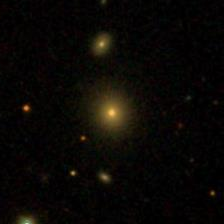
\includegraphics[width=\linewidth]{figures/foundations/elliptical.png}\\
\small (a) Ellittica
\end{minipage}\hfill
\begin{minipage}{0.31\textwidth}
\centering
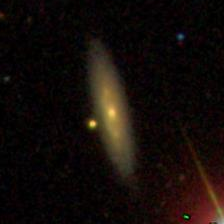
\includegraphics[width=\linewidth]{figures/foundations/spiral.png}\\
\small (b) Spirale
\end{minipage}\hfill
\begin{minipage}{0.31\textwidth}
\centering
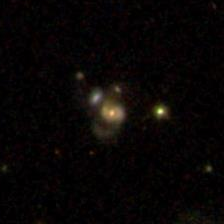
\includegraphics[width=\linewidth]{figures/foundations/merger.png}\\
\small (c) Sistema etichettato merger
\end{minipage}
\caption{Esempi reali del dataset derivato da immagini SDSS e classificazioni
Galaxy Zoo. Sono mostrati ritagli centrali di \(224\times224\) pixel,
senza sovrapposizioni interpretative. Gli identificativi degli oggetti sono,
da sinistra, \texttt{1237656241699881339}, \texttt{1237651273507668077} e
\texttt{1237655499209310435}. Gli esempi sono illustrativi, non prototipi
esaustivi delle classi; l'etichetta merger non costituisce da sola una
conferma fisica di fusione.}
\label{fig:fond-esempi}
\end{figure}

\subsection{Survey, annotazioni e difficoltà del riconoscimento}

Le survey astronomiche producono raccolte di immagini per le quali
l'ispezione individuale non è facilmente scalabile. Galaxy Zoo ha affrontato
il problema coinvolgendo volontari nella classificazione delle immagini
SDSS; il rilascio Galaxy Zoo 1 rende disponibili classificazioni
morfologiche aggregate per un ampio campione di galassie
\cite{lintott2011galaxyzoo}. Le frazioni di voto descrivono le risposte
dei classificatori e il loro accordo: non vanno identificate automaticamente
con probabilità fisiche certe di appartenenza a una classe.

Risoluzione, rapporto segnale-rumore, orientamento e presenza di sorgenti
vicine influenzano ciò che è riconoscibile nell'immagine. Inoltre, una
distribuzione luminosa perturbata può essere più difficile da descrivere
con una singola etichetta. Ciò motiva l'uso della classe merger come
ulteriore banco di prova, senza assumere a priori che essa debba essere
sempre la più difficile per qualsiasi modello.

Il passaggio da due a tre classi modifica sia le decisioni richieste sia
la composizione del problema. Non equivale a modificare un solo parametro
di difficoltà mantenendo invariato tutto il resto. Soglie di voto,
bilanciamento e separazione degli oggetti tra training e test devono
quindi essere esplicitati, come avviene nel \cref{chap:dataset}.

\section{Apprendimento profondo e transfer learning}
\label{sec:fond-transfer}

\subsection{Reti convoluzionali e rappresentazioni delle immagini}

Una rete convoluzionale elabora un'immagine mediante filtri applicati a
regioni locali, condividendo gli stessi pesi tra posizioni diverse.
Le uscite sono mappe di attivazione: ciascun canale risponde a determinati
pattern appresi durante l'addestramento. La composizione di strati
convoluzionali e trasformazioni non lineari consente di combinare
informazioni locali in rappresentazioni progressivamente più elaborate.

Non è necessario definire manualmente una misura per ogni possibile
struttura morfologica. Tuttavia, non è neppure corretto attribuire
automaticamente a ogni attivazione un significato astronomico preciso:
una feature appresa può mescolare forma, colore, tessitura e informazioni
legate al processo osservativo. L'impiego delle CNN nella classificazione
galattica è esemplificato da Dieleman et al.~\cite{dieleman2015galaxy},
che incorporano le simmetrie delle immagini nel modello di riconoscimento.

Una distinzione utile è quella tra \emph{estrattore di feature}, che
trasforma l'immagine in una rappresentazione, e \emph{testa di
classificazione}, che usa tale rappresentazione per produrre i punteggi
delle classi. Questa separazione permette di studiare teste diverse
senza modificare ogni volta l'intero sistema di visione.

\subsection{Reti residuali e ResNet18}

Le reti residuali introducono collegamenti che sommano l'ingresso di
un blocco alla trasformazione appresa dal blocco stesso
\cite{he2016resnet}. Quando le dimensioni coincidono, il principio è
espresso da
\begin{equation}
 \boldsymbol y=F(\boldsymbol x;\boldsymbol w)+\boldsymbol x.
\end{equation}
Il blocco apprende così una correzione rispetto alla rappresentazione
in ingresso. Quando cambiano le dimensioni, il collegamento può includere
una proiezione. Queste connessioni facilitano l'ottimizzazione di reti
profonde, senza garantire da sole una migliore generalizzazione per
qualunque dataset.

ResNet18 è una variante relativamente compatta della famiglia. Eliminando
il classificatore finale si ottiene, dopo l'aggregazione spaziale delle
mappe, un vettore di 512 componenti. Nel presente lavoro questa
rappresentazione costituisce il punto di partenza comune dei modelli.
Il numero 512 indica la dimensione del vettore, non un elenco di 512
proprietà fisiche delle galassie note a priori.

\subsection{Preaddestramento, congelamento e fine-tuning}

Il transfer learning riutilizza una rappresentazione appresa su un
problema sorgente per affrontarne un altro. È possibile aggiornare
anche i pesi dell'estrattore sul nuovo dataset, effettuando
\emph{fine-tuning}, oppure mantenerli fissi e addestrare soltanto la testa.
La seconda strategia riduce il numero di parametri da stimare e consente
di riutilizzare le feature già calcolate.

Il riuso di feature apprese su immagini naturali non implica che esse
siano ottimali per immagini astronomiche. È una scelta sperimentale
che introduce un limite, ma permette anche un confronto più controllato:
le differenze tra teste non dipendono da backbone addestrati separatamente.
Nel presente lavoro ResNet18 è preaddestrata su ImageNet e congelata; il
trasferimento al dominio galattico avviene attraverso gli strati successivi.
Di conseguenza, la componente quantistica riceve feature classiche
compresse, non direttamente i pixel dell'immagine.

\section{Fondamenti di calcolo quantistico}
\label{sec:fond-quantum}

Si richiamano qui le nozioni del modello a circuito necessarie per
leggere l'architettura ibrida. Per una trattazione sistematica di stati,
porte e misure si rimanda a Nielsen e Chuang~\cite{nielsen2010quantum}.

\subsection{Qubit e registri quantistici}

Un qubit è descritto, nel caso di uno stato puro, da un vettore normalizzato
in uno spazio complesso bidimensionale:
\begin{equation}
 |\psi\rangle=\alpha|0\rangle+\beta|1\rangle,
 \qquad \alpha,\beta\in\mathbb C,
 \qquad |\alpha|^2+|\beta|^2=1.
\end{equation}
I vettori \(|0\rangle\) e \(|1\rangle\) formano la base computazionale.
Una misura in questa base restituisce 0 oppure 1, con probabilità
rispettivamente \(|\alpha|^2\) e \(|\beta|^2\). La sovrapposizione
descrive lo stato prima della misura: non significa poter leggere
simultaneamente entrambi i valori come due bit classici.

Per \(q\) qubit lo spazio degli stati è il prodotto tensoriale degli
spazi dei singoli qubit e ha dimensione \(2^q\). Uno stato puro generale è
\begin{equation}
 |\psi\rangle=\sum_{z=0}^{2^q-1}c_z|z\rangle,
 \qquad \sum_z|c_z|^2=1.
\end{equation}
La crescita dello spazio delle ampiezze è importante, ma non dimostra
un vantaggio nell'apprendimento: preparazione dello stato, trasformazioni
realizzabili e modalità di lettura limitano l'informazione accessibile.

\subsection{Porte, rotazioni ed entanglement}

Nel modello ideale a circuito, le porte trasformano lo stato mediante
operatori unitari. Le rotazioni impiegate in questa tesi sono
\begin{equation}
 R_Y(a)=
 \begin{pmatrix}\cos(a/2)&-\sin(a/2)\\
 \sin(a/2)&\cos(a/2)\end{pmatrix},
 \qquad
 R_Z(b)=
 \begin{pmatrix}e^{-ib/2}&0\\0&e^{ib/2}\end{pmatrix}.
\end{equation}
Applicata a \(|0\rangle\), la prima produce
\(\cos(a/2)|0\rangle+\sin(a/2)|1\rangle\): un angolo classico
controlla quindi le ampiezze dello stato. La seconda agisce sulle fasi;
il suo effetto sulle probabilità osservate dipende anche dalle operazioni
successive, che possono convertire differenze di fase in differenze
misurabili.

La porta CNOT coinvolge un qubit di controllo e uno bersaglio:
\begin{equation}
 \operatorname{CNOT}|c,t\rangle=|c,t\oplus c\rangle,
 \qquad c,t\in\{0,1\},
\end{equation}
dove \(\oplus\) è la somma modulo due. Su opportune sovrapposizioni
può generare entanglement. Per uno stato puro, questo significa che lo
stato congiunto non è esprimibile come prodotto degli stati dei singoli
sottosistemi. La presenza di una CNOT non garantisce però che ogni input
generi uno stato entangled, né che tali correlazioni migliorino la
classificazione.

\subsection{Misure e valori attesi}

Per usare il circuito in un classificatore occorre ottenere uscite
numeriche. La misura dell'osservabile di Pauli
\(Z=\operatorname{diag}(1,-1)\) ha esiti \(+1\) e \(-1\). Il suo
valore atteso sul qubit \(i\) è
\begin{equation}
 z_i=\langle\psi|Z_i|\psi\rangle
     =P_i(0)-P_i(1),\qquad z_i\in[-1,1],
\end{equation}
dove \(Z_i\) agisce sul qubit considerato e come identità sugli altri.
Leggendo un'osservabile per qubit si ottiene un vettore reale di
dimensione \(q\), senza ricostruire tutte le \(2^q\) ampiezze.

Su hardware, un valore atteso è normalmente stimato ripetendo preparazione
e misura per un numero finito di esecuzioni, dette \emph{shot}. Una
simulazione ideale dello stato può invece calcolarlo direttamente, senza
rumore di campionamento delle misure. Questa distinzione è essenziale
per interpretare sia il training sia i costi.

\section{Reti neurali ibride classico-quantistiche}
\label{sec:fond-ibrido}

\subsection{Encoding delle feature}

Un circuito destinato a elaborare dati classici richiede una mappa di
codifica. Nell'\emph{angle encoding} le componenti di un vettore
determinano gli angoli delle porte. Per esempio,
\begin{equation}
 |\phi(\boldsymbol a)\rangle=
 \left[\bigotimes_{i=1}^{q}R_Y(a_i)\right]|0\rangle^{\otimes q}.
\end{equation}
La codifica non assegna una classe a ciascun qubit: tutti i valori in
uscita possono contribuire alla decisione su ciascuna classe.

Quando le feature iniziali sono più numerose dei qubit, una trasformazione
classica può comprimerle e limitarne l'intervallo prima dell'encoding.
Questa proiezione è parte del modello e può essere addestrabile.
La rappresentazione risultante va distinta dall'\emph{amplitude encoding},
nel quale i dati sono codificati nelle ampiezze di uno stato normalizzato.
Le strategie comportano operazioni e costi diversi e non sono
intercambiabili senza modificare il modello.

Un'altra distinzione riguarda il \emph{data re-uploading}, che inserisce
nuovamente i dati in più punti del circuito. Il circuito principale
della tesi usa invece un solo blocco iniziale di encoding; la ripetizione
degli strati parametrizzati non equivale a ripetere la codifica dei dati.

\subsection{Circuiti variazionali e architettura ibrida}

Un circuito variazionale applica una trasformazione
\(U(\boldsymbol\theta)\) con parametri regolabili. La disposizione
delle porte e dei collegamenti, detta \emph{ansatz}, definisce la famiglia
di trasformazioni esplorata durante il training. È utile distinguere
gli angoli \(\boldsymbol a\), che dipendono dall'esempio, dai pesi
\(\boldsymbol\theta\), condivisi tra gli esempi e aggiornati
dall'ottimizzatore.

Nel paradigma ibrido una rete classica prepara gli ingressi del circuito
e una seconda trasformazione ne elabora le letture. Mari et al.
\cite{mari2020transfer} formalizzano questo schema nel contesto del
transfer learning. Una scrittura generale è
\begin{equation}
 \boldsymbol\ell(x)=h_{\boldsymbol\omega}
 \left(\boldsymbol z_{\boldsymbol\theta}
 \left(g_{\boldsymbol\eta}(F_{\mathrm{pre}}(x))\right)\right),
\end{equation}
dove \(F_{\mathrm{pre}}\) è l'estrattore preaddestrato,
\(g_{\boldsymbol\eta}\) la proiezione classica,
\(\boldsymbol z_{\boldsymbol\theta}\) il vettore dei valori attesi e
\(h_{\boldsymbol\omega}\) la testa finale. Le componenti di
\(\boldsymbol\ell\) sono punteggi, detti \emph{logit}, convertibili
in probabilità mediante softmax. Le letture quantistiche non sono
quindi, da sole, probabilità delle classi.

\begin{figure}[tbp]
\centering
\resizebox{\textwidth}{!}{% Schema originale: solo TikZ e arrows.meta, gia' nel preambolo.
\begin{tikzpicture}[
 box/.style={draw=black!55,rounded corners=2pt,align=center,
 text width=2.15cm,minimum height=1cm,font=\small,inner sep=5pt},
 flow/.style={-{Latex[length=2mm]},draw=black!65,thick}]
\node[box,fill=black!3] (image) at (0,0) {Immagine\\\(x\)};
\node[box,fill=black!3] (backbone) at (3.1,0)
 {Estrattore classico\\congelato};
\node[box,fill=blue!5] (pre) at (6.2,0)
 {Proiezione\\\(\boldsymbol a=g_{\boldsymbol\eta}(\boldsymbol f)\)};
\node[box,fill=violet!8] (quantum) at (9.3,0)
 {Blocco quantistico\\\(\boldsymbol z_{\boldsymbol\theta}(\boldsymbol a)\)};
\node[box,fill=blue!5] (head) at (12.4,0)
 {Classificatore\\logit di classe};
\draw[flow] (image) -- (backbone);
\draw[flow] (backbone) -- node[above,font=\small]{\(\boldsymbol f\)} (pre);
\draw[flow] (pre) -- (quantum);
\draw[flow] (quantum) -- (head);
\node[box,fill=violet!3] (encode) at (6.2,-2.1)
 {Encoding\\\(R_Y(a_i)\)};
\node[box,fill=violet!8] (unitary) at (9.3,-2.1)
 {Trasformazione\\\(U(\boldsymbol\theta)\)};
\node[box,fill=violet!3] (readout) at (12.4,-2.1)
 {Lettura\\\(\langle Z_1\rangle,\ldots,\langle Z_q\rangle\)};
\draw[flow] (encode) -- (unitary);
\draw[flow] (unitary) -- (readout);
\draw[dashed,draw=black!40] (quantum.south) -- (unitary.north);
\node[align=left,font=\small,text width=3.8cm] at (1.1,-2.1)
 {Dettaglio funzionale\\del blocco quantistico};
\end{tikzpicture}
}
\caption{Schema concettuale di un classificatore ibrido con estrattore
congelato. Il dettaglio inferiore distingue encoding dipendente dai dati,
trasformazione variazionale e lettura. Si tratta di uno schema funzionale,
non del circuito specifico implementato, descritto nel \cref{chap:modelli}.}
\label{fig:fond-ibrido}
\end{figure}

\subsection{Addestramento e circuito congelato}

La funzione di perdita confronta le predizioni con le etichette e guida
l'aggiornamento dei parametri addestrabili. Per ottimizzare la proiezione
classica occorre derivare la perdita anche rispetto agli ingressi del
circuito. La catena di derivate collega quindi componenti classiche e
quantistiche; non si tratta di addestrare due classificatori indipendenti.

Su simulatori differenziabili è possibile usare la differenziazione
automatica. Su hardware, per opportune porte parametrizzate, regole come
il \emph{parameter-shift} permettono di ricavare derivate da valutazioni
del circuito con parametri traslati \cite{schuld2019gradients}. Le due
modalità non hanno lo stesso costo operativo; quella effettivamente
adottata è precisata nel \cref{chap:modelli}.

Congelare \(\boldsymbol\theta\) lascia invece fissa la trasformazione
circuitale. Il modello può continuare ad apprendere attraverso
\(\boldsymbol\eta\) e \(\boldsymbol\omega\), e le uscite del circuito
continuano a cambiare al cambiare dell'input. Questo controllo consente
di distinguere il contributo dell'inserimento del circuito da quello
dell'ottimizzazione dei suoi pesi.

\subsection{Simulazione e processori quantistici}

La simulazione classica consente di valutare il comportamento matematico
di un circuito, ma non ne riproduce necessariamente il costo su un
processore quantistico. Una simulazione generica a vettore di stato
memorizza \(2^q\) ampiezze complesse; il costo dipende anche dal numero
e dal tipo di porte, dal batch e dal metodo di differenziazione.
Non si può quindi attribuire ogni differenza temporale al solo numero
di parametri addestrabili.

In questa tesi le operazioni quantistiche sono simulate e i valori attesi
sono calcolati senza shot finiti. Non si modellano rumore del dispositivo,
errori di lettura o vincoli di accesso a una QPU. L'esperimento studia
il comportamento predittivo delle architetture e il costo della loro
implementazione simulata, non un'accelerazione ottenuta su hardware
quantistico.

\section{Potenzialità, limiti e criteri di confronto}
\label{sec:fond-confronto}

\subsection{Espressività, generalizzazione e ottimizzazione}

L'espressività riguarda le funzioni rappresentabili da un modello;
la generalizzazione riguarda le prestazioni su esempi non usati per
addestrarlo. Una famiglia più ampia non garantisce una generalizzazione
migliore: contano dati disponibili, regolarizzazione e procedura di
ottimizzazione. Anche un numero ridotto di pesi non implica automaticamente
un vantaggio nei regimi con pochi esempi.

Per i circuiti quantistici, McClean et al.~\cite{mcclean2018barren}
mostrano che determinate famiglie di circuiti e condizioni di
inizializzazione possono produrre gradienti la cui varianza si riduce
esponenzialmente con il numero di qubit. Queste regioni del paesaggio di
ottimizzazione sono dette \emph{barren plateau}. Il fenomeno costituisce
un limite teorico importante, ma non è una spiegazione automatica di
ogni risultato negativo. Non è sufficiente osservare una Macro-F1 bassa
per diagnosticarlo, soprattutto in circuiti piccoli e poco profondi:
servono analisi specifiche dei gradienti e delle condizioni teoriche.

\subsection{Baseline, ablazioni e significato del vantaggio}

Un modello ibrido deve essere confrontato con controlli che permettano
di distinguere l'effetto del circuito da quello di altre scelte. Una
baseline lineare descrive quanto le classi siano linearmente separabili
nello spazio delle feature; una
testa non lineare offre un riferimento più flessibile; un bottleneck
classico della stessa dimensione controlla la compressione. Un'ablazione
con circuito congelato verifica invece il contributo
dell'addestramento dei parametri quantistici.

Capacità comparabile non significa equivalenza delle famiglie funzionali.
Condividere dimensioni e inizializzazioni di alcuni strati riduce le
differenze non pertinenti alla domanda di ricerca, ma non rende i modelli
identici per espressività o ottimizzabilità. Bowles et al.
\cite{bowles2024benchmarking} sottolineano l'importanza delle baseline
e del disegno sperimentale nel valutare modelli di quantum machine
learning, mostrando quanto sia limitante una lettura basata sulla sola
graduatoria delle prestazioni.

Un \emph{vantaggio predittivo} richiede un miglioramento valutato su dati
non usati per selezionare il modello e rispetto a riferimenti adeguati.
Un \emph{vantaggio computazionale} riguarda invece risorse e costi
necessari per ottenere un risultato comparabile. Le due nozioni non
coincidono. Per questo la tesi considera congiuntamente classificazione,
qualità delle probabilità e tempi, con le metriche e gli indicatori
statistici definiti nel \cref{chap:modelli}. La prestazione di un singolo
seed non è sufficiente a caratterizzare un'architettura.

\section{Lavori correlati e posizionamento della tesi}
\label{sec:fond-correlati}

\subsection{Dalla classificazione visuale alle reti profonde}

Galaxy Zoo fornisce un collegamento tra annotazione visuale e analisi
automatica, rendendo disponibili etichette aggregate per immagini
astronomiche \cite{lintott2011galaxyzoo}. Dieleman et al.
\cite{dieleman2015galaxy} mostrano come reti convoluzionali progettate
tenendo conto delle rotazioni possano apprendere la classificazione
morfologica dalle annotazioni. Il loro problema di predizione e la
struttura delle etichette non coincidono però con le tre classi operative
della presente tesi: i punteggi non costituiscono un confronto numerico
diretto con i nostri risultati.

In questo lavoro il backbone preaddestrato rimane fisso. L'analisi si
concentra sulla testa e sulla trasformazione applicata alle feature
compresse, mantenendo comune la rappresentazione fornita ai modelli.

\subsection{Transfer learning classico-quantistico}

Mari et al.~\cite{mari2020transfer} costituiscono il riferimento
architetturale per combinare un estrattore classico preaddestrato con
un circuito variazionale e strati classici di interfaccia. L'interesse
è rendere utilizzabili piccoli registri quantistici su rappresentazioni
di immagini ad alta dimensionalità. Questa fattibilità non implica,
da sola, che il circuito superi una testa classica ben controllata.

Otgonbaatar et al.~\cite{otgonbaatar2023transfer} studiano il transfer
learning quantistico su dataset reali di telerilevamento, anche piccoli
e ad alta dimensionalità. Il contesto motiva l'attenzione alla scarsità
di dati, ma non consente di trasferire direttamente conclusioni al
dominio galattico. Differiscono caratteristiche delle immagini,
etichette e configurazioni circuitali.

Kim et al.~\cite{kim2023transfer} considerano invece il trasferimento
verso reti convoluzionali quantistiche. È importante distinguere questa
impostazione dalla nostra: nel presente studio convoluzioni ed estrazione
spaziale rimangono classiche; il circuito interviene soltanto sul vettore
di feature compresso. L'espressione rete ibrida non identifica quindi
un'unica architettura.

\subsection{Contributo sperimentale del lavoro}

Il lavoro si colloca tra queste proposte architetturali e l'esigenza di
una valutazione controllata. Lo studio di Bowles et al.
\cite{bowles2024benchmarking} offre un riferimento metodologico per
interrogare il ruolo effettivo delle componenti quantistiche. Anche
in questo caso task e modelli differiscono: non si usa il risultato
di altri benchmark per anticipare l'esito del nostro esperimento.

La tesi studia una rappresentazione classica comune, controlli con
bottleneck di pari dimensione e circuiti sia addestrabili sia congelati.
Il confronto è ripetuto su due task e su diversi regimi di disponibilità
del training, distinguendo evidenze principali e analisi esplorative.
L'obiettivo non è assumere un vantaggio quantistico, ma individuare
se e in quali condizioni il circuito apporti un beneficio rispetto
alle alternative classiche e a quale costo. I capitoli successivi
traducono questa domanda in un dataset verificabile e in un protocollo
sperimentale riproducibile.

\chapter{Dataset e protocollo di validazione}
\label{chap:dataset}

Per confrontare i classificatori classici e ibridi, i modelli devono
essere valutati sugli stessi esempi. Questo capitolo descrive la
costruzione del dataset, dalla selezione del catalogo alle partizioni
di training, validation e test. Sono riportati i controlli usati per
garantire l'appaiamento e i limiti del campione selezionato.

Il dataset finale comprende \(5\,628\) immagini, suddivise in tre classi
bilanciate: galassie ellittiche, galassie spirali e sistemi classificati
come \emph{merger}.
A partire da questo insieme si definiscono
un problema binario, limitato alle ellittiche e alle spirali, e un
problema a tre classi, che include anche i merger. L’introduzione di
questi ultimi consente di valutare i modelli in uno scenario di
maggiore complessità morfologica, verificando se le differenze tra
classificatori classici e quantistici emergano più chiaramente
rispetto al caso binario. La valutazione si basa su dieci
ripetizioni di un holdout stratificato. Per ciascuna ripetizione
vengono costruiti sottoinsiemi stratificati del training set, al fine di
analizzare l’impatto della disponibilità dei dati.

\section{Provenienza dei dati e popolazione selezionata}
\label{sec:provenienza}

Le immagini e i metadati provengono dai servizi dello Sloan Digital Sky
Survey (SDSS), utilizzati attraverso la Data Release 17
(DR17)~\cite{abdurrouf2022dr17}. Le informazioni morfologiche sono quelle
di Galaxy Zoo presenti nella tabella \texttt{zooSpec}: il servizio di accesso
è DR17, ma ciò non implica che le classificazioni morfologiche siano state
prodotte originariamente per questa release. Galaxy Zoo raccoglie
classificazioni visuali collaborative, successivamente sintetizzate in
frazioni di voto e indicatori morfologici~\cite{lintott2011galaxyzoo}.

L'estrazione del catalogo è stata effettuata mediante una query CasJobs
che collega \texttt{PhotoObj}, \texttt{zooSpec} e \texttt{SpecObj}. Sono
richiesti il flag fotometrico \texttt{clean=1}, la classificazione
\texttt{type=3}, una magnitudine nella banda \(g\) compresa tra \(14\) e
\(17{,}5\) e un redshift compreso tra \(0{,}005\) e \(0{,}1\).
La query, riportata nell'\cref{app:query}, usa l'operatore
\texttt{BETWEEN}, che include gli estremi; il successivo controllo locale
sul redshift applica invece \(0{,}005<z<0{,}1\).

Il file esportato conserva identificativo dell'oggetto, ascensione retta,
declinazione, redshift e tre indicatori morfologici. Non conserva invece
le colonne \texttt{clean}, \texttt{type} e \(g\). I relativi vincoli sono
quindi documentati dalla query di estrazione, ma non possono essere
verificati nuovamente a partire dal solo CSV locale. Questa distinzione
separa la provenienza documentata dai controlli effettivamente ripetibili
sugli artefatti distribuiti.

La popolazione risultante non costituisce un campione indiscriminato di
tutte le galassie SDSS: disponibilità spettroscopica, intervallo di
magnitudine, redshift e selezione morfologica ne delimitano il campo di
validità. Le prestazioni misurate nella tesi si riferiscono a questa
popolazione selezionata.

\section{Assegnazione delle etichette}
\label{sec:etichette}

Per ellittiche e spirali vengono utilizzati rispettivamente
\texttt{p\_el\_debiased} e \texttt{p\_cs\_debiased}; per i merger viene
utilizzato \texttt{p\_mg}. Le prime due quantità includono una correzione
dei bias osservativi nella classificazione, mentre l'indicatore merger
ha una diversa origine nella struttura dei voti. Non è quindi opportuno
interpretare le tre soglie come livelli omogenei di probabilità calibrata
o come garanzie di correttezza della singola etichetta. Il ruolo delle
classificazioni Galaxy Zoo e dell'indicatore di fusione è discusso nei
lavori di rilascio e di selezione dei sistemi interagenti
\cite{lintott2011galaxyzoo,darg2010mergers}.

Le soglie operative sono riportate nella \cref{tab:soglie}. Indicando con
\(p_c\) l'indicatore della classe \(c\) e con \(\tau_c\) la soglia
corrispondente, un oggetto riceve un'etichetta soltanto se
\begin{equation}
  \sum_{c\in\{\mathrm{E},\mathrm{M},\mathrm{S}\}}
  \mathbf{1}\{p_c>\tau_c\}=1.
  \label{eq:etichetta-univoca}
\end{equation}
L'etichetta assegnata è quella dell'unica condizione soddisfatta. Un oggetto
che non supera alcuna soglia, oppure ne supera più di una, non viene
ammesso come esempio etichettato. La query effettua una prima selezione
con un'unione logica delle condizioni; il requisito di unicità viene
applicato nella costruzione locale del manifest.

\begin{table}[tbp]
\centering
\caption{Regole di etichettatura. Le disuguaglianze sono strette; deve
essere soddisfatta esattamente una delle tre condizioni.}
\label{tab:soglie}
\begin{tabular}{lll}
\toprule
\rowcolor{ThesisTableHeader}
\tablehead{Classe} & \tablehead{Indicatore nel catalogo} & \tablehead{Condizione} \\
\midrule
Ellittica & \texttt{p\_el\_debiased} & \(p_{\mathrm{E}}>0{,}8\) \\
Merger & \texttt{p\_mg} & \(p_{\mathrm{M}}>0{,}4\) \\
Spirale & \texttt{p\_cs\_debiased} & \(p_{\mathrm{S}}>0{,}8\) \\
\bottomrule
\end{tabular}
\end{table}

La \cref{fig:voti} mostra le distribuzioni degli indicatori utilizzati
per assegnare l'etichetta nei candidati selezionati. Le soglie definiscono
il problema supervisionato, ma non eliminano il rumore delle etichette.
In particolare, la categoria merger è un'etichetta operativa derivata
dal catalogo: la procedura non comprende una nuova revisione visuale
esperta di ogni sistema. Né il superamento della soglia \(0{,}4\)
riproduce automaticamente tutte le ulteriori selezioni di cataloghi
specialistici di fusioni.

\begin{figure}[tbp]
\centering
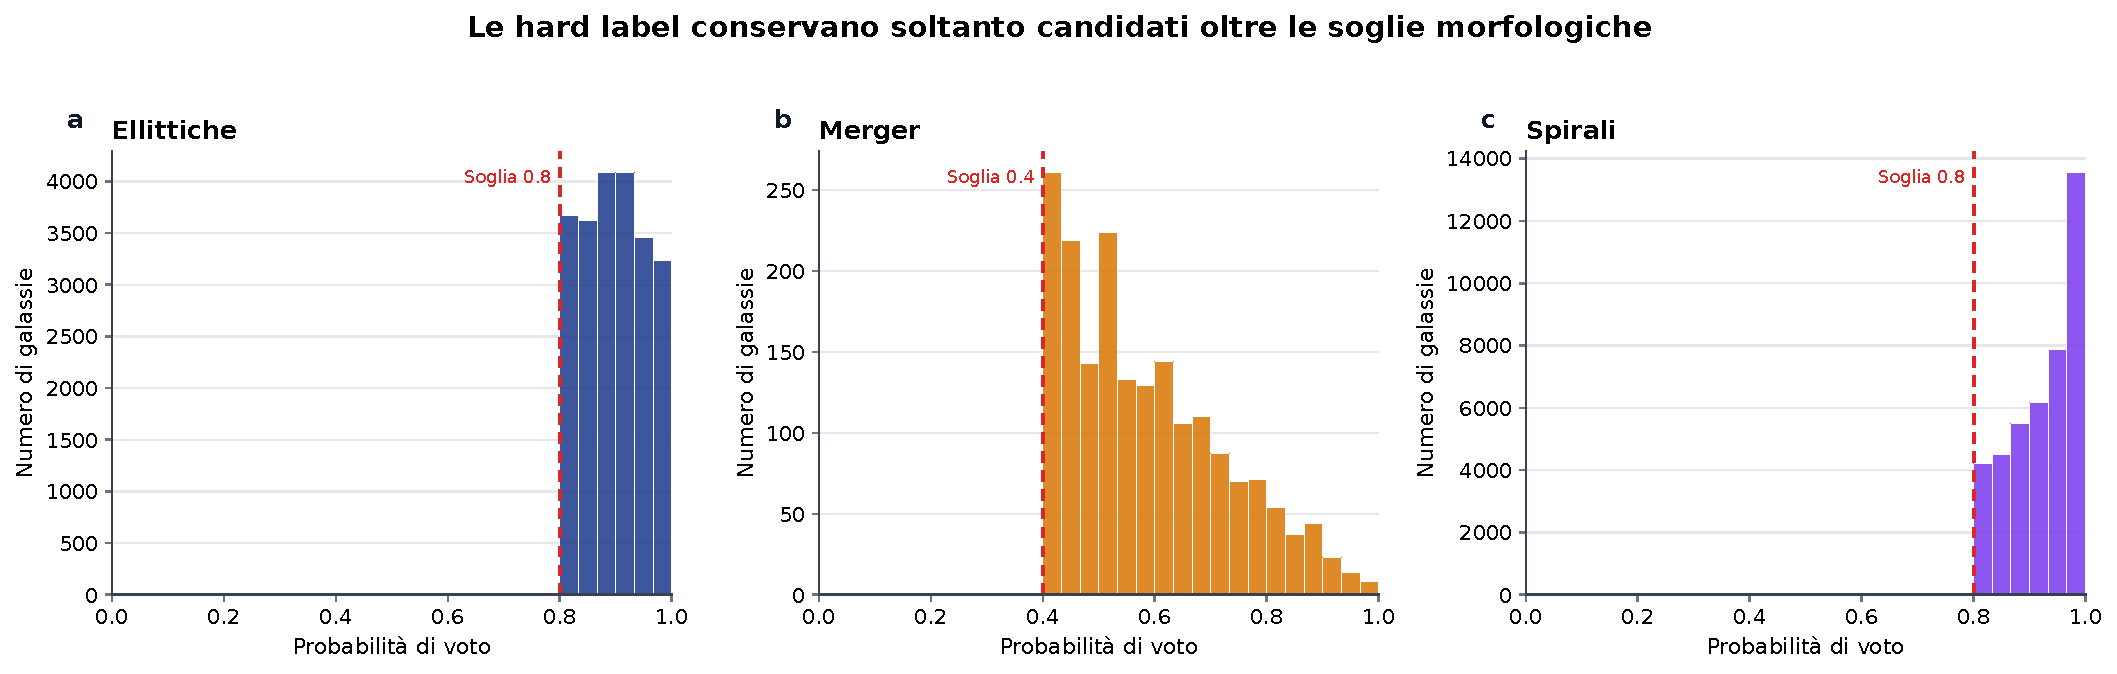
\includegraphics[width=\textwidth]{03_vote_fractions.pdf}
\caption{Distribuzione degli indicatori morfologici nei candidati
selezionati, separati secondo la classe assegnata. Le linee verticali
indicano le soglie operative: \(0{,}8\) per ellittiche e spirali,
\(0{,}4\) per merger. Le distribuzioni sono già condizionate dalla
selezione e non rappresentano l'intero catalogo sorgente.}
\label{fig:voti}
\end{figure}

\section{Pulizia, acquisizione e bilanciamento}
\label{sec:pulizia}

\subsection{Integrità del catalogo}

Il catalogo esportato contiene \(65\,906\) righe. La pulizia rimuove
cinque duplicati esatti e \(72\) righe associate a \(36\) identificativi
discordanti. Per questi ultimi vengono escluse tutte le occorrenze,
anziché scegliere arbitrariamente una delle versioni. Rimangono
\(65\,829\) candidati: \(22\,163\) ellittiche, \(1\,877\) merger e
\(41\,789\) spirali.

Gli identificativi SDSS \texttt{objid} vengono conservati come stringhe.
Questa scelta evita gli arrotondamenti che possono essere introdotti
dalla conversione in numeri a virgola mobile di identificativi con molte
cifre. L'identificativo viene usato come chiave nei manifest, nelle
partizioni e nelle predizioni: una sua alterazione comprometterebbe sia
la tracciabilità sia i controlli di sovrapposizione.

\subsection{Pool di acquisizione e controlli sulle immagini}

La classe merger, con \(1\,877\) candidati, determina la scala del
bilanciamento. Per disporre di una riserva in caso di download non riusciti
o immagini non valide, il pool di acquisizione comprende tutti i merger
e \(2\,347\) oggetti per ciascuna delle altre due classi:
\[
  2\,347=\left\lceil 1{,}25\cdot1\,877\right\rceil.
\]
Il campionamento utilizza il seed di progetto \(42\). Il pool contiene
complessivamente \(6\,571\) oggetti, senza richiedere il download di
tutti i candidati del catalogo.

Per ogni oggetto viene richiesto al servizio SDSS un ritaglio
(\emph{cutout}) JPEG RGB di \(320\times320\) pixel, centrato sulle
coordinate catalogate, con scala di \(0{,}396\) secondi d'arco per pixel.
Il lato dell'immagine corrisponde quindi a circa \(126{,}7\) secondi
d'arco. Si tratta di immagini di visualizzazione a colori, non di un
addestramento direttamente sui dati fotometrici grezzi delle singole bande.

La validazione verifica leggibilità e integrità del file, dimensioni,
modalità RGB, dimensione minima di \(512\) byte e variabilità della
luminanza. Quest'ultima è calcolata dai canali RGB tramite
\[
  Y=0{,}2126R+0{,}7152G+0{,}0722B;
\]
è richiesta una deviazione standard di almeno \(1\), sulla scala
\(0\)--\(255\), per individuare immagini sostanzialmente uniformi.
Tutti i \(6\,571\) cutout del pool superano i controlli.

Viene inoltre calcolata l'impronta SHA-256 dei file per rilevare
duplicati identici a livello di byte, sia entro una classe sia tra
classi diverse. Nel pool validato non emergono duplicati di questo tipo.
Il controllo non equivale tuttavia a una deduplicazione percettiva:
due immagini dello stesso sistema con ritagli o codifiche differenti
possono avere hash diversi. Analogamente, identificativi distinti non
garantiscono che due cutout non includano porzioni di cielo comuni.

\subsection{Dataset finale}

Il numero finale per classe è fissato a \(1\,876\), arrotondando
\(1\,877\) al multiplo di quattro inferiore. Questo consente quote
stratificate esatte per la successiva ripartizione \(50/25/25\).
Il campionamento finale è deterministico e usa il seed di progetto con
un offset dipendente dalla classe.

La \cref{tab:dataset-numeri} e la \cref{fig:attrition} riepilogano le
numerosità. Dei \(6\,571\) file validi, \(943\) non entrano nel campione
finale: \(471\) ellittiche, un merger e \(471\) spirali. Queste esclusioni
derivano dal bilanciamento e non da un fallimento dei controlli di qualità.

\begin{table}[tbp]
\centering
\caption{Numerosità nelle principali fasi della costruzione del dataset.
Il pool validato coincide con quello acquisito; il passaggio finale
riduce il campione per bilanciamento.}
\label{tab:dataset-numeri}
\begin{tabular}{lrrrr}
\toprule
\rowcolor{ThesisTableHeader}
\tablehead{Fase} & \tablehead{Ellittiche} & \tablehead{Merger} & \tablehead{Spirali} & \tablehead{Totale} \\
\midrule
Candidati puliti & \(22\,163\) & \(1\,877\) & \(41\,789\) & \(65\,829\) \\
Pool acquisito & \(2\,347\) & \(1\,877\) & \(2\,347\) & \(6\,571\) \\
Immagini valide & \(2\,347\) & \(1\,877\) & \(2\,347\) & \(6\,571\) \\
Dataset finale & \(1\,876\) & \(1\,876\) & \(1\,876\) & \(5\,628\) \\
\bottomrule
\end{tabular}
\end{table}

\begin{figure}[tbp]
\centering
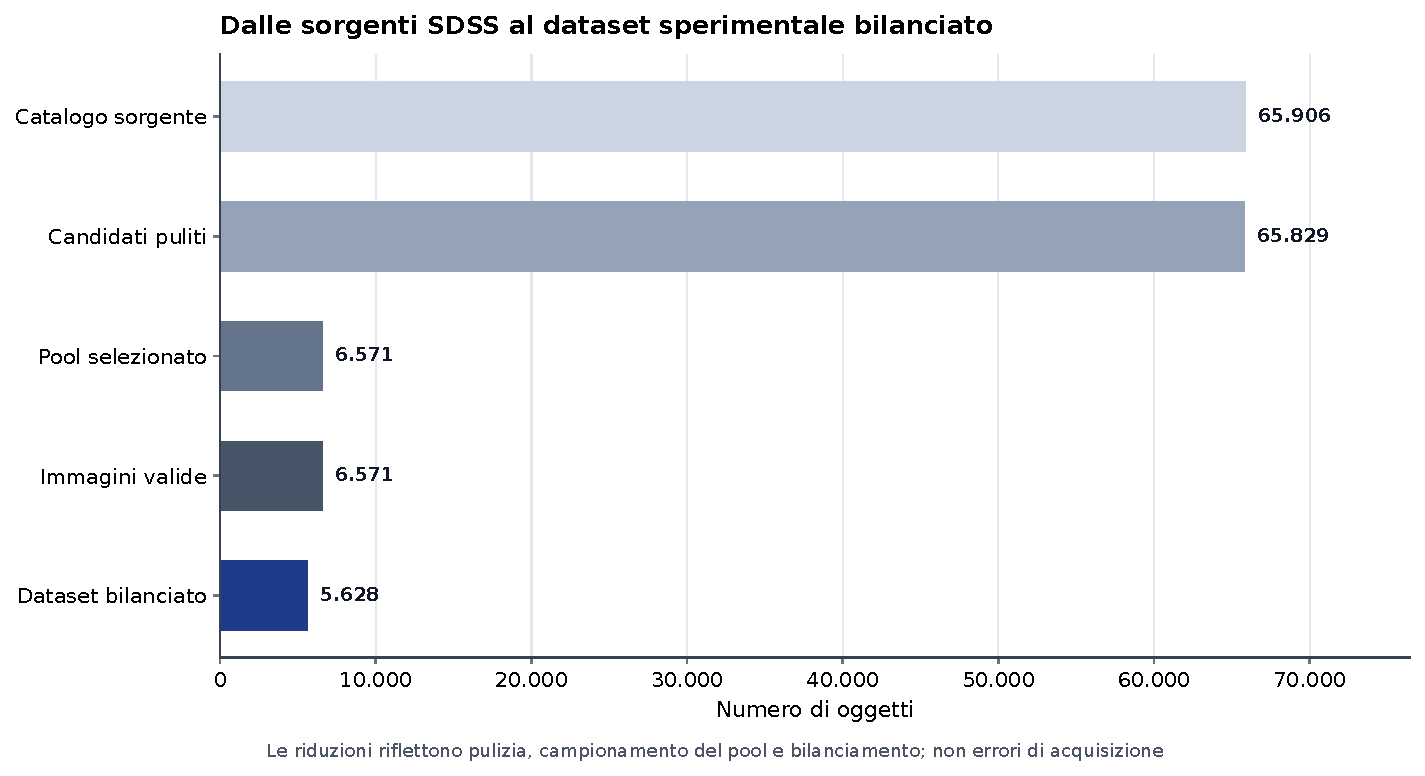
\includegraphics[width=\textwidth]{01_data_attrition.pdf}
\caption{Numerosità lungo la pipeline: catalogo esportato, candidati
puliti, pool di download, immagini valide e dataset finale. La riduzione
tra candidati e pool è una selezione pianificata; quella tra immagini
valide e dataset finale dipende dal bilanciamento.}
\label{fig:attrition}
\end{figure}

Il cambiamento della composizione di classe è illustrato nella
\cref{fig:bilanciamento}. Il bilanciamento facilita il confronto tra
classi e impedisce che la numerosità molto maggiore delle spirali
domini l'addestramento. Modifica però la prevalenza rispetto al catalogo:
metriche aggregate e probabilità prodotte dal classificatore non possono
essere trasferite automaticamente a una popolazione astronomica con
frequenze diverse.

\begin{figure}[tbp]
\centering
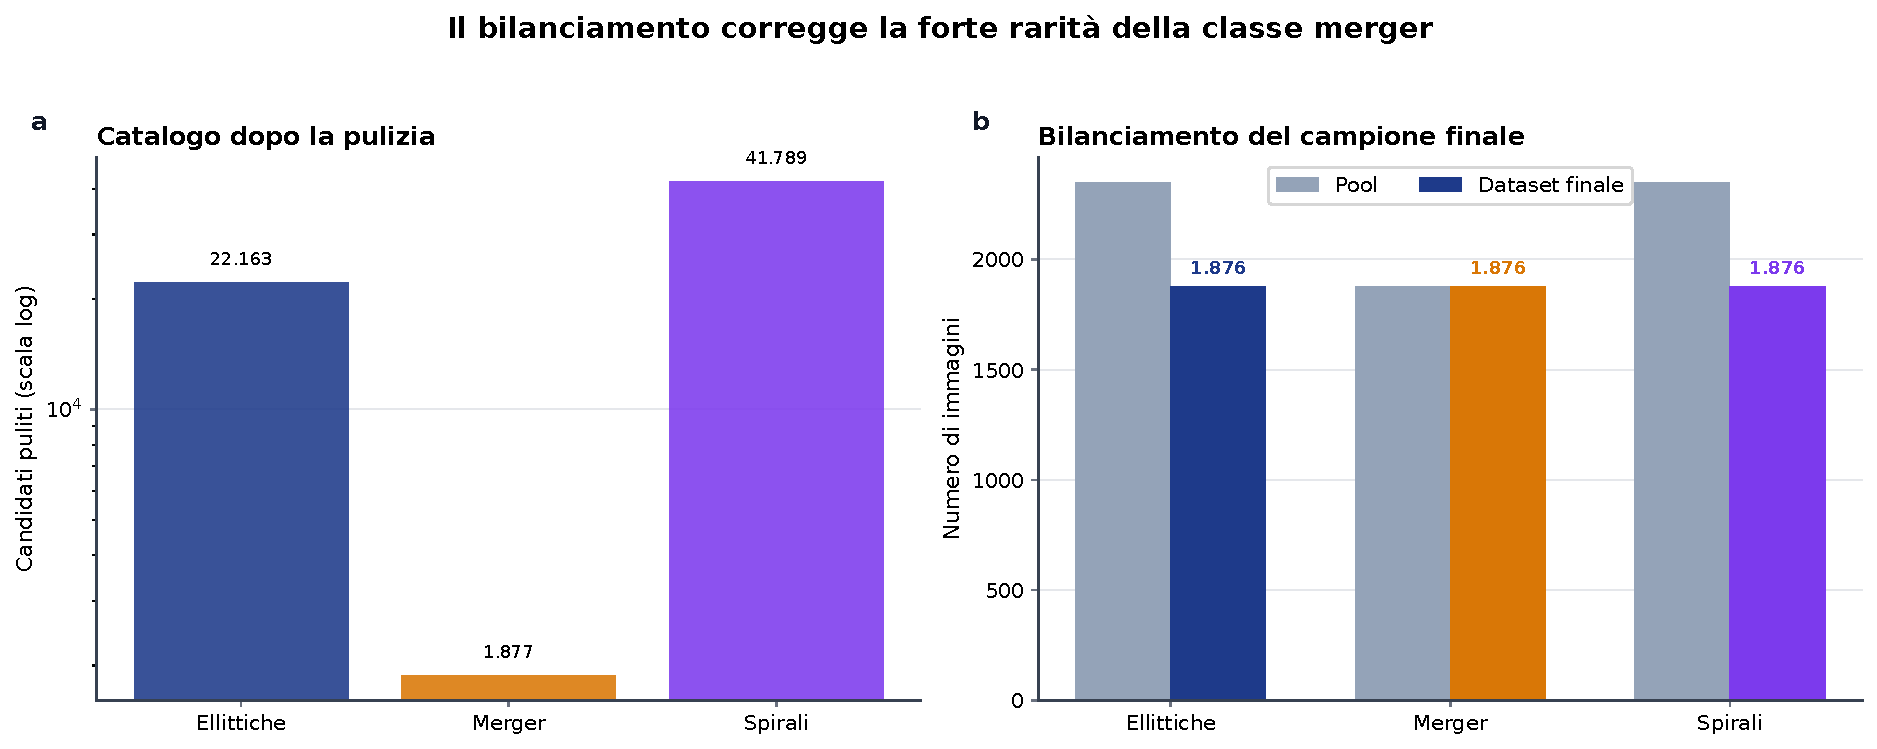
\includegraphics[width=\textwidth]{02_class_balance.pdf}
\caption{Composizione per classe dei candidati, del pool di acquisizione
e del dataset finale. Il pannello dei candidati utilizza una scala
logaritmica. Il campione finale contiene \(1\,876\) oggetti per classe;
questa distribuzione è una scelta sperimentale, non una stima della
prevalenza delle morfologie nella popolazione SDSS.}
\label{fig:bilanciamento}
\end{figure}

\section{Caratteristiche del campione e trasformazioni}
\label{sec:trasformazioni}

\subsection{Redshift e limiti del controllo osservativo}

La \cref{fig:redshift} descrive il redshift delle tre classi nel dataset
finale. Il bilanciamento numerico non rende identiche le distribuzioni
delle altre proprietà: le classi mantengono distribuzioni di redshift
differenti. La figura è una descrizione del campione, non un test di
significatività né una dimostrazione che il redshift causi gli errori
del classificatore.

\begin{figure}[tbp]
\centering
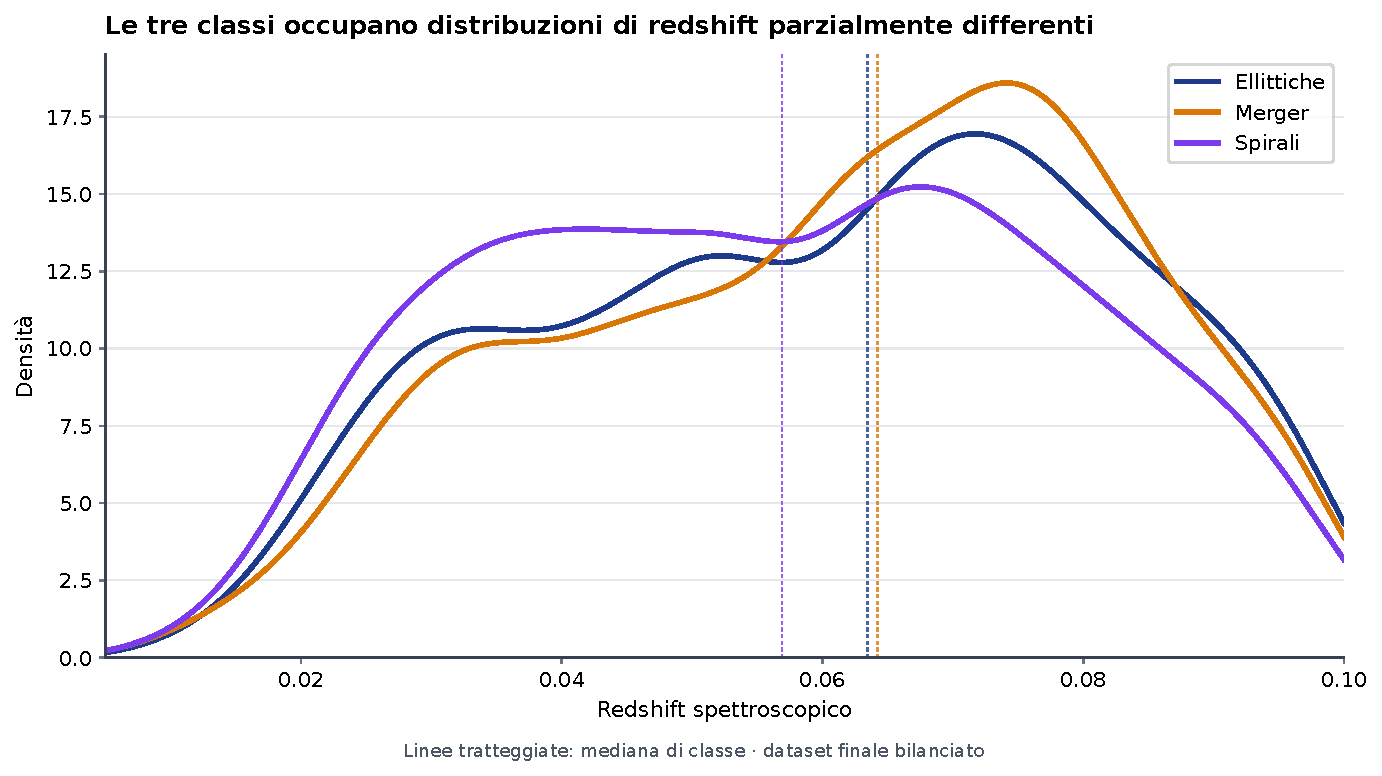
\includegraphics[width=\textwidth]{04_redshift_distribution.pdf}
\caption{Distribuzione del redshift nel dataset finale, distinta per
classe. Le curve rappresentano stime di densità; le linee verticali
indicano le mediane. La selezione nell'intervallo
\(0{,}005<z<0{,}1\) non comporta un abbinamento delle distribuzioni di
redshift tra classi.}
\label{fig:redshift}
\end{figure}

Coordinate, redshift e frazioni di voto sono usati per costruzione e audit
del dataset, non come input aggiuntivi del classificatore. Ciò non esclude
che proprietà correlate a questi metadati, come dimensione apparente o
risoluzione delle strutture, siano presenti nelle immagini. Non è stato
applicato un abbinamento tra classi per redshift o dimensione angolare.
Questo aspetto delimita l'interpretazione astronomica dei risultati.

\subsection{Preprocessing e rappresentazione condivisa}

Le immagini di training sono ruotate di un angolo casuale tra
\(0^\circ\) e \(360^\circ\), con interpolazione bilineare, quindi
ritagliate centralmente a \(224\times224\) pixel. Seguono riflessioni
orizzontali e verticali, ciascuna con probabilità \(0{,}5\).
Il ritaglio viene effettuato dopo la rotazione: il buffer iniziale
da \(320\) pixel consente di mantenere il quadrato centrale senza i bordi
neri introdotti agli angoli. In particolare,
\(320/\sqrt{2}\simeq226{,}3>224\).

I valori vengono convertiti in tensori e normalizzati per canale con
medie \((0{,}485,0{,}456,0{,}406)\) e deviazioni standard
\((0{,}229,0{,}224,0{,}225)\), coerentemente con i pesi ImageNet
utilizzati. Validation e test impiegano soltanto ritaglio centrale,
conversione e normalizzazione, senza trasformazioni casuali.

Le immagini così trasformate sono elaborate da una ResNet18
\cite{he2016resnet} con pesi \texttt{IMAGENET1K\_V1} di
TorchVision~\cite{torchvisionresnet18}. Il classificatore finale viene
rimosso e ogni immagine è rappresentata da un vettore di \(512\) feature.
Il backbone è congelato e utilizzato in modalità di valutazione:
l'esperimento confronta pertanto classificatori che ricevono una
rappresentazione classica condivisa, non backbone addestrati separatamente.

Le feature sono precalcolate e conservate in una cache per ripetizione.
Nella procedura utilizzata, l'augmentation del training produce una
vista per oggetto al momento della costruzione della cache: tale vista
rimane fissa nelle epoche successive. Non si tratta quindi di una nuova
rotazione a ogni epoca. La condivisione della cache mantiene costante
anche questa componente del confronto tra modelli. Il dettaglio delle
teste classiche e quantistiche è rinviato al \cref{chap:modelli}.

\section{Task e repeated holdout stratificato}
\label{sec:holdout}

Il task a tre classi utilizza tutte le immagini del dataset finale.
Il task binario considera soltanto ellittiche e spirali, escludendo
i merger e rimappando le etichette a due classi. Le partizioni binarie
derivano dal filtraggio delle corrispondenti partizioni a tre classi:
gli oggetti delle due classi comuni mantengono dunque il proprio ruolo
di training, validation o test nella stessa ripetizione.

Per ciascun repeat seed il campione viene suddiviso in tre insiemi
disgiunti: \(50\%\) per l'addestramento, \(25\%\) per la validazione e
\(25\%\) per il test. La stratificazione preserva il bilanciamento
tra classi in ogni insieme. Le numerosità sono riportate nella
\cref{tab:split}.

\begin{table}[tbp]
\centering
\caption{Numerosità per ciascuna ripetizione del protocollo.
Nella riga per classe i conteggi valgono per ciascuna classe presente
nel task. La denominazione \texttt{full} indica la colonna Training.}
\label{tab:split}
\begin{tabular}{lrrrr}
\toprule
\rowcolor{ThesisTableHeader}
\tablehead{Task} & \tablehead{Training} & \tablehead{Validation} & \tablehead{Test} & \tablehead{Totale} \\
\midrule
Binario & \(1\,876\) & \(938\) & \(938\) & \(3\,752\) \\
Tre classi & \(2\,814\) & \(1\,407\) & \(1\,407\) & \(5\,628\) \\
Per classe & \(938\) & \(469\) & \(469\) & \(1\,876\) \\
\bottomrule
\end{tabular}
\end{table}

I dieci repeat seed utilizzati sono
\[
  42,\;314,\;2718,\;1618,\;2026,\;7,\;73,\;137,\;1729,\;4096.
\]
Ogni seed definisce una ripetizione riproducibile. Tutti i modelli
condividono le stesse partizioni all'interno della ripetizione: il
confronto delle prestazioni viene così effettuato sugli stessi oggetti
di test e con gli stessi dati disponibili per l'apprendimento.

L'implementazione costruisce quattro blocchi stratificati di uguale
dimensione, con mescolamento determinato dal seed, e ne assegna due al
training, uno alla validation e uno al test. L'esperimento conserva
esclusivamente la prima assegnazione, identificata negli artefatti da
\texttt{iteration=1}. Le altre rotazioni non contribuiscono ai risultati
della tesi. Il protocollo effettivamente valutato è quindi un
\emph{repeated holdout stratificato}, non una cross-validation completa
a quattro fold.

La validation è impiegata per monitorare l'apprendimento e selezionare
il checkpoint secondo il criterio definito nel
\cref{chap:modelli}; il test è riservato alla valutazione del modello
selezionato. La separazione tra questi ruoli evita che il test venga
usato come criterio operativo di arresto dell'addestramento.

La disgiunzione vale entro ciascuna ripetizione. Tra ripetizioni diverse
uno stesso oggetto può invece comparire più volte nel test, oppure
cambiare ruolo. I dieci risultati misurano quindi la variabilità del
protocollo sul medesimo dataset, non quella di dieci campioni astronomici
indipendenti. Questa dipendenza va tenuta presente nell'interpretazione
degli intervalli e impedisce di trattare tutte le predizioni concatenate
come osservazioni indipendenti.

\section{Regimi a ridotta disponibilità di dati}
\label{sec:subset}

Per studiare il comportamento in condizioni \emph{low-resource}, il
training set viene ridotto a \(100\), \(300\) e \(900\) immagini
complessive. Il numero indica il totale del sottoinsieme, non il numero
per classe. Validation e test restano invariati rispetto alla
ripetizione \texttt{full}: una variazione delle prestazioni non dipende
quindi dalla sostituzione del campione su cui vengono misurate.

La selezione è bilanciata, salvo gli inevitabili arrotondamenti.
Nel task binario i tre regimi contengono rispettivamente \(50\), \(150\)
e \(450\) immagini per classe; nel task a tre classi, il regime da
\(100\) immagini contiene \(33\), \(33\) e \(34\) esempi, mentre quelli
da \(300\) e \(900\) ne contengono rispettivamente \(100\) e \(300\)
per classe.

Per ciascuna combinazione di task e repeat seed, ogni sottoinsieme
è selezionato esclusivamente dal training completo:
\begin{equation}
  \mathcal{T}_{n}^{(s)}\subset\mathcal{T}_{\mathrm{full}}^{(s)},
  \qquad n\in\{100,300,900\}.
  \label{eq:subset-training}
\end{equation}
La selezione usa un seed condiviso tra i modelli:
un controllo classico e il corrispondente classificatore quantistico
non vengono addestrati su campioni estratti separatamente.

Il \cref{lst:training-subset} riporta il nucleo di
\texttt{select\_training\_subset}, in \texttt{scripts/train.py},
con i ritorni a capo adattati. Sono omessi import, gestione del regime
Full e costruzione del contenitore di uscita. La selezione avviene per
identificativo di oggetto, non per singola vista aumentata.

\begin{code}
\begin{minted}{python}
requested = int(subset_size)
identities = bank.metadata[["objid", "label"]].drop_duplicates("objid")
if requested >= len(identities):
    return bank
selected, _ = train_test_split(
    identities, train_size=requested,
    stratify=identities["label"], random_state=seed
)
mask = bank.metadata["objid"].isin(selected["objid"])
metadata = bank.metadata.loc[mask].reset_index(drop=True).copy()
features = bank.features[torch.from_numpy(mask.to_numpy())]
metadata["feature_index"] = range(len(metadata))
\end{minted}
\caption{Selezione stratificata dei soli dati di training.}
\label{lst:training-subset}
\end{code}

Nel notebook di esecuzione dei subset, il seed di selezione è quello
\texttt{dataloader}, condiviso dalle architetture. Il codice conservato
effettua una chiamata separata per ciascuna numerosità: non impone
esplicitamente l'inclusione del campione da 100 in quello da 300 e
di quest'ultimo in quello da 900. Inoltre, il riepilogo denominato
\texttt{nested\_audit} registra le numerosità, ma non verifica tali
inclusioni. Non si assume pertanto un annidamento reciproco dimostrato.
Le curve descrivono l'effetto del regime di campionamento; le differenze
possono dipendere anche dalla composizione del sottoinsieme, oltre che
dalla numerosità e dalla variabilità dell'ottimizzazione.

Il regime \texttt{full} corrisponde a \(1\,876\) immagini di training nel
binario e a \(2\,814\) nel task a tre classi. Nei grafici comparativi
questa etichetta deve dunque essere distinta da una numerosità universale.
Le curve rispetto a \(100\), \(300\), \(900\) e \texttt{full} descrivono
l'effetto della quantità di dati, non l'andamento della loss nelle epoche.

\section{Tracciabilità e perimetro delle conclusioni}
\label{sec:tracciabilita}

La pipeline conserva manifest del catalogo, download, validazione e
campione finale, insieme alle assegnazioni dei singoli oggetti alle
partizioni. Gli artefatti di ogni run comprendono configurazione,
cronologia dell'addestramento, checkpoint, metriche e predizioni.
Il collegamento tramite identificativi consente di ricondurre una metrica
aggregata agli esempi valutati e di verificare l'appaiamento tra modelli.

Ai fini del confronto sperimentale, i principali controlli sono
l'unicità degli identificativi nel campione, la verifica degli hash,
la separazione dei ruoli entro ciascun holdout, la condivisione delle
feature e l'invarianza di validation e test nei regimi ridotti.
Questi controlli non sostituiscono una validazione esterna. Rimangono
possibili rumore nelle etichette, differenze osservazionali tra classi
e correlazioni tra oggetti astronomicamente vicini; non viene effettuata
una suddivisione per gruppi di sistemi fisici o regioni di cielo.

Il protocollo consente pertanto di studiare l'effetto della scelta del
classificatore su una rappresentazione e su partizioni controllate.
Non misura, da solo, la capacità di generalizzare a survey differenti
o a una popolazione con diversa prevalenza morfologica. Su questa base,
il capitolo successivo definisce le architetture, le condizioni di
addestramento e i confronti statistici con cui vengono valutate le
domande di ricerca.

\chapter{Modelli e disegno sperimentale}
\label{chap:modelli}

Il protocollo del \cref{chap:dataset} mantiene controllati gli oggetti
utilizzati per addestramento e valutazione. Su questa base, il presente
capitolo definisce che cosa viene modificato nel passaggio dal modello
classico a quello quantistico e quali condizioni rimangono invariate.
La domanda non è se una rete contenente un circuito quantistico possa
classificare immagini, ma se quel circuito apporti un beneficio rispetto
a un controllo classico che attraversa lo stesso collo di bottiglia.

\section{Impostazione del confronto}
\label{sec:disegno-confronto}

\subsection{Una rappresentazione classica comune}

Tutti i modelli ricevono un vettore \(\boldsymbol{f}\in\mathbb{R}^{512}\)
prodotto dalla stessa ResNet18 congelata, secondo il preprocessing e la
procedura di caching già descritti. Non viene effettuato un fine-tuning
del backbone sul dataset galattico. I parametri ottimizzati appartengono
esclusivamente alla testa di classificazione.

Il \cref{lst:feature-backbone} mostra la costruzione dell'estrattore
in \texttt{models/classical.py}. La sostituzione di \texttt{fc}
con l'identità restituisce le 512 feature invece dei logit ImageNet.
Durante il caching, \texttt{data/features.py} pone l'estrattore in
modalità \texttt{eval()} ed esegue l'inferenza entro
\texttt{torch.no\_grad()}. Le teste sono poi addestrate sulle feature
salvate: il backbone non appartiene al loro grafo di ottimizzazione.

\begin{code}
\begin{minted}{python}
def resnet18_backbone(*, pretrained: bool = True) -> nn.Module:
    weights = models.ResNet18_Weights.IMAGENET1K_V1 if pretrained else None
    backbone = models.resnet18(weights=weights)
    backbone.fc = nn.Identity()
    return backbone
\end{minted}
\caption{Costruzione della ResNet18 usata per il caching delle feature;
negli esperimenti viene selezionato \texttt{pretrained=True}.}
\label{lst:feature-backbone}
\end{code}

L'architettura ibrida segue il paradigma del \emph{dressed quantum
circuit}: una trasformazione classica prepara l'input del circuito e
un'altra ne converte l'uscita nei punteggi di classe. Mari et al.
\cite{mari2020transfer} hanno proposto questo schema nell'ambito del
transfer learning classico-quantistico. Nel telerilevamento, Otgonbaatar
et al.~\cite{otgonbaatar2023transfer} hanno studiato un'impostazione
basata su feature classiche e piccoli circuiti, considerando anche
varianti con data re-uploading. Questi lavori motivano il tipo di
architettura, non garantiscono un miglioramento nel diverso problema
affrontato qui.

Il modello della tesi non applica convoluzioni quantistiche ai pixel e
non include operazioni di pooling quantistico. È quindi distinto dalle
QCNN con strati di convoluzione e pooling, come quelle considerate da
Kim et al.~\cite{kim2023transfer}: la parte convoluzionale rimane
interamente classica.

\subsection{Ruolo delle famiglie di modelli}

Le baseline B0 e B1 forniscono due riferimenti contestuali: una testa
lineare e un percettrone multistrato. Il confronto centrale riguarda
invece B2, Q e QF. B2 è una testa classica con bottleneck di quattro o
otto componenti; Q inserisce, dopo la stessa compressione, un circuito
variazionale addestrabile; QF mantiene identico il circuito, ma ne
congela i parametri interni.

Questa separazione permette di distinguere tre domande. B0 e B1
indicano quanto le feature siano sfruttabili da classificatori classici.
Il confronto Q--B2 valuta l'inserimento del circuito a parità di
dimensione del bottleneck. Il confronto Q--QF studia il contributo
dell'ottimizzazione dei pesi circuitali, rispetto a una trasformazione
quantistica fissata all'inizializzazione. La \cref{fig:pipeline-modelli}
riassume la struttura del confronto principale.

\begin{figure}[tbp]
\centering
% Schema originale della struttura implementata: nessuna figura di articoli copiata.
\begin{tikzpicture}[
  font=\footnotesize,
  block/.style={draw=black!50,rounded corners=2pt,align=center,
    minimum height=0.95cm,text width=2.15cm,inner sep=4pt},
  flow/.style={-{Latex[length=2mm]},draw=black!55,line width=0.65pt}
]
\node[block,fill=black!3] (features) at (0,0)
  {ResNet18 congelata\\feature \(\boldsymbol f\in\mathbb R^{512}\)};
\foreach \row/\modelname/\yy in {b/B2/2,q/Q/0,f/QF/-2}{
  \node[block] (pre\row) at (3.1,\yy)
    {Proiezione + \(\pi\tanh\)\\\(512\rightarrow q\)};
  \node[anchor=south,yshift=2pt,font=\footnotesize\bfseries] at (pre\row.north) {\modelname};
  \node[block] (post\row) at (9.5,\yy)
    {Classificatore affine\\\(q\rightarrow K\)};
  \draw[flow] (features.east) -- (pre\row.west);
}
\node[block,fill=blue!5] (midb) at (6.3,2)
  {Nessun circuito\\Uscita: \(\boldsymbol a\)};
\node[block,fill=violet!7] (midq) at (6.3,0)
  {Circuito \(+\langle Z\rangle\)\\\(\boldsymbol\theta\) addestrabile};
\node[block,fill=orange!9] (midf) at (6.3,-2)
  {Circuito \(+\langle Z\rangle\)\\\(\boldsymbol\theta\) congelato};
\foreach \row in {b,q,f}{
  \draw[flow] (pre\row.east) -- (mid\row.west);
  \draw[flow] (mid\row.east) -- (post\row.west);
}
\end{tikzpicture}

\caption{Struttura delle teste B2, Q e QF. Le feature \(\boldsymbol f\)
sono condivise. Proiezione e classificatore hanno la stessa forma e
gli stessi valori iniziali nelle tre configurazioni appaiate; durante
il training vengono ottimizzati separatamente. In QF rimane fisso
soltanto il tensore \(\boldsymbol\theta\) del circuito.}
\label{fig:pipeline-modelli}
\end{figure}

\section{Teste classiche}
\label{sec:teste-classiche}

Si indica con \(K\in\{2,3\}\) il numero di classi e con
\(\boldsymbol{\ell}\in\mathbb{R}^{K}\) il vettore dei \emph{logit},
ossia i punteggi non normalizzati prodotti dalla rete. Le probabilità
sono ottenute mediante
\begin{equation}
  p_k=\frac{\exp(\ell_k)}{\sum_{c=1}^{K}\exp(\ell_c)},
  \qquad \widehat y=\mathop{\mathrm{arg\,max}}_k p_k.
  \label{eq:softmax-modelli}
\end{equation}
Anche nel caso binario vengono prodotti due logit e utilizzata la softmax.

\subsection{B0: classificatore lineare}

La baseline B0 applica una trasformazione affine direttamente alle
feature:
\begin{equation}
  \boldsymbol{\ell}_{\mathrm{B0}}
  =W_0\boldsymbol f+\boldsymbol b_0,
  \qquad W_0\in\mathbb{R}^{K\times512}.
\end{equation}
Il modello verifica quanto il problema sia separabile linearmente nella
rappresentazione preaddestrata. La sua semplicità riguarda la testa:
l'intera pipeline comprende comunque un backbone convoluzionale profondo.

\subsection{B1: percettrone multistrato}

B1 introduce uno strato nascosto di \(512\) unità con attivazione ReLU
e dropout di probabilità \(0{,}3\):
\begin{equation}
  \boldsymbol{\ell}_{\mathrm{B1}}
  =W_2\,D_{0{,}3}\!\left(\mathrm{ReLU}
    (W_1\boldsymbol f+\boldsymbol b_1)\right)+\boldsymbol b_2.
\end{equation}
Il dropout è attivo durante l'addestramento e disattivato in valutazione.
B1 non impone la compressione a quattro o otto componenti e dispone
di molti più parametri delle teste del confronto centrale. Per questo
costituisce un riferimento di contesto, non un controllo a capacità
comparabile del circuito.

\subsection{B2: controllo con bottleneck condiviso}

Per \(q\in\{4,8\}\), B2 calcola
\begin{align}
  \boldsymbol a &= \pi\tanh(W_{\mathrm{in}}\boldsymbol f+
                       \boldsymbol b_{\mathrm{in}}),
                       \label{eq:compressione-angoli}\\
  \boldsymbol{\ell}_{\mathrm{B2}}
                &=W_{\mathrm{out}}\boldsymbol a+
                       \boldsymbol b_{\mathrm{out}},
                       \label{eq:baseline-b2}
\end{align}
dove \(W_{\mathrm{in}}\in\mathbb{R}^{q\times512}\) e
\(W_{\mathrm{out}}\in\mathbb{R}^{K\times q}\).
La tangente iperbolica agisce componente per componente e limita
l'input del blocco successivo all'intervallo \((-\pi,\pi)\).

In B2, \(q\) indica esclusivamente una dimensione classica: il modello
non contiene qubit. La corrispondenza con Q e QF riguarda la dimensione,
la trasformazione di compressione e la struttura del classificatore.
Il controllo non sostituisce il circuito con una rete classica arbitraria
di dimensione maggiore.

\section{Classificatore ibrido e circuito variazionale}
\label{sec:circuito-primario}

\subsection{Encoding delle feature compresse}

Q e QF utilizzano la stessa trasformazione della
\cref{eq:compressione-angoli}. L'input quantistico è quindi il vettore
\(\boldsymbol a\in(-\pi,\pi)^q\), non il vettore originale di \(512\)
feature né l'immagine. I qubit sono inizializzati in
\(\lvert0\rangle^{\otimes q}\). La codifica applica una rotazione
\(R_Y(a_j)\) al qubit \(j\):
\begin{equation}
  U_{\mathrm{enc}}(\boldsymbol a)
   =\bigotimes_{j=0}^{q-1} R_Y(a_j),\qquad
  R_Y(a)=
  \begin{pmatrix}
   \cos(a/2)&-\sin(a/2)\\
   \sin(a/2)&\cos(a/2)
  \end{pmatrix}.
  \label{eq:encoding-ry}
\end{equation}
Prima dell'entanglement lo stato è un prodotto:
\[
  U_{\mathrm{enc}}(\boldsymbol a)\lvert0\rangle^{\otimes q}
   =\bigotimes_{j=0}^{q-1}
     \left[\cos(a_j/2)\lvert0\rangle+
           \sin(a_j/2)\lvert1\rangle\right].
\]
Ogni componente compressa determina dunque una rotazione locale.
La compressione è appresa dalla rete e non coincide con una selezione
manuale di quattro o otto descrittori astronomici.

\subsection{Ansatz e ordine delle operazioni}

Il circuito impiega \(L=2\) blocchi variazionali. In ciascun blocco,
su ogni qubit si applicano prima \(R_Z(\theta_{\ell j0})\) e poi
\(R_Y(\theta_{\ell j1})\). Segue una catena di CNOT nelle direzioni
\[
  0\longrightarrow1,\quad1\longrightarrow2,\quad\ldots,\quad
  q-2\longrightarrow q-1,
\]
eseguite nell'ordine indicato. Non è presente una CNOT di chiusura
dall'ultimo al primo qubit.

Per rendere esplicito l'ordine matriciale, si definiscono
\begin{align}
 V_\ell(\boldsymbol\theta_\ell)
   &=\bigotimes_{j=0}^{q-1}
       R_Y(\theta_{\ell j1})R_Z(\theta_{\ell j0}),\\
 E&=\mathrm{CNOT}_{q-2,q-1}\cdots
       \mathrm{CNOT}_{1,2}\mathrm{CNOT}_{0,1}.
\end{align}
Gli operatori a destra agiscono per primi. Lo stato finale è
\begin{equation}
 \lvert\psi(\boldsymbol a,\boldsymbol\theta)\rangle
 =E V_2(\boldsymbol\theta_2)\,
  E V_1(\boldsymbol\theta_1)\,
  U_{\mathrm{enc}}(\boldsymbol a)\lvert0\rangle^{\otimes q}.
 \label{eq:stato-finale}
\end{equation}

La \cref{fig:circuito-q4} mostra il blocco per quattro qubit.
L'encoding compare una sola volta: aumentare il numero di blocchi
variazionali non significa reintrodurre i dati a ogni blocco.
Il circuito primario non utilizza quindi data re-uploading, amplitude
encoding o il template \texttt{BasicEntanglerLayers}.

\begin{figure}[tbp]
\centering
% Il blocco tratteggiato è ripetuto in sequenza, non in parallelo.
\begin{tikzpicture}[
  x=1cm,y=0.9cm,font=\footnotesize,
  gate/.style={draw=black!65,fill=white,minimum height=0.55cm,
    minimum width=1.12cm,inner sep=2pt}
]
\draw[dashed,rounded corners=3pt,draw=violet!60!black]
  (2.15,0.65) rectangle (7.3,-3.65);
\node[anchor=south,align=center] at (4.725,0.7)
  {Blocco \(\ell\): ripetere per \(\ell=1,2\)};
\foreach \j in {0,1,2,3}{
  \draw[black!55] (0,-\j) -- (9.6,-\j);
  \node[anchor=east] at (0,-\j) {\(\lvert0\rangle_{\j}\)};
  \node[gate,fill=blue!5] at (1.1,-\j) {\(R_Y(a_{\j})\)};
  \node[gate] at (3,-\j) {\(R_Z(\theta_{\ell\j0})\)};
  \node[gate] at (4.4,-\j) {\(R_Y(\theta_{\ell\j1})\)};
  \node[gate,fill=black!3] at (8.45,-\j) {\(\langle Z_{\j}\rangle\)};
}
\foreach \x/\control/\target in {5.45/0/1,6.1/1/2,6.75/2/3}{
  \draw (\x,-\control) -- (\x,-\target);
  \fill (\x,-\control) circle (2pt);
  \draw[fill=white] (\x,-\target) circle (4pt);
  \draw (\x-0.14,-\target) -- (\x+0.14,-\target);
  \draw (\x,-\target-0.155) -- (\x,-\target+0.155);
}
\node[anchor=north] at (1.1,-3.9) {Encoding unico};
\node[anchor=north] at (8.45,-3.9) {Lettura};
\end{tikzpicture}

\caption{Circuito a quattro qubit. L'encoding \(R_Y(a_j)\) viene
eseguito una volta; il riquadro tratteggiato viene ripetuto due volte,
con parametri diversi nei due blocchi. Le CNOT formano una catena
aperta nell'ordine da sinistra a destra. L'uscita comprende i quattro
valori attesi locali di Pauli-\(Z\).}
\label{fig:circuito-q4}
\end{figure}

Il tensore variazionale ha forma \(L\times q\times2\), per un totale
di \(2Lq\) parametri: \(16\) con quattro qubit e \(32\) con otto.
Il numero di CNOT è \(L(q-1)\), rispettivamente \(6\) e \(14\).
La dimensione dello spazio di Hilbert passa da \(2^4=16\) a
\(2^8=256\), ma questi numeri non indicano né il numero di immagini
memorizzabili né il numero di feature classiche indipendenti fornite
all'encoding. La crescita dello spazio degli stati non costituisce,
da sola, una garanzia di capacità utile o di generalizzazione.

\subsection{Lettura e classificazione}

Dal circuito vengono estratti i valori attesi
\begin{equation}
  z_j=
  \langle\psi(\boldsymbol a,\boldsymbol\theta)|
     Z_j|\psi(\boldsymbol a,\boldsymbol\theta)\rangle,
  \qquad j=0,\ldots,q-1.
  \label{eq:lettura-z}
\end{equation}
Il vettore \(\boldsymbol z\in[-1,1]^q\) alimenta un classificatore affine:
\[
  \boldsymbol\ell_{\mathrm Q}
    =W_{\mathrm{out}}\boldsymbol z+\boldsymbol b_{\mathrm{out}}.
\]
Le probabilità di classe derivano dalla softmax, non direttamente dalla
misura di un singolo qubit. In particolare, gli otto qubit della variante
più grande non corrispondono a otto classi.

\subsection{QF: circuito congelato, rete ancora addestrabile}
\label{sec:qf}

QF ha la stessa espressione di Q, ma il tensore
\(\boldsymbol\theta\) resta fisso ai valori iniziali. Proiezione
\(W_{\mathrm{in}},\boldsymbol b_{\mathrm{in}}\) e classificatore
\(W_{\mathrm{out}},\boldsymbol b_{\mathrm{out}}\) rimangono addestrabili.
Il circuito continua quindi a elaborare input che cambiano durante
l'ottimizzazione.

Congelare i pesi non interrompe il gradiente rispetto agli angoli.
La regola della catena contiene infatti il contributo
\[
  \frac{\partial\mathcal L}{\partial W_{\mathrm{in}}}
  =\frac{\partial\mathcal L}{\partial\boldsymbol z}
    \frac{\partial\boldsymbol z}{\partial\boldsymbol a}
    \frac{\partial\boldsymbol a}{\partial W_{\mathrm{in}}},
\]
che deve essere calcolato anche in QF. Non è pertanto corretto attendersi
che il costo del circuito congelato scompaia. L'implementazione esclude
i pesi quantistici dall'ottimizzatore e ne controlla il checksum durante
il training.

Il confronto Q--QF valuta il beneficio dell'ottimizzazione circuitale
all'interno di questo sistema congiunto. Non isola invece l'effetto
dell'entanglement: entrambi i modelli contengono le stesse CNOT.

\subsection{Passaggi essenziali dell'implementazione}
\label{sec:snippet-reti}

I listati seguenti collegano la descrizione matematica al codice
effettivamente utilizzato. Sono estratti dei moduli
\texttt{models/classical.py} e \texttt{models/pennylane\_qnn.py}
del package \texttt{tesi\_qml}, con ritorni a capo adattati alla pagina.
Non sono programmi autonomi: import, costruttori e gestione dei dati
sono omessi. In particolare, \texttt{scale\_angles} applica
\(\pi\tanh\) nella configurazione degli esperimenti.

Il ramo attivo della funzione \texttt{scale\_angles} e la proiezione
del costruttore sono riportati nel \cref{lst:angle-projection}.
I frammenti appartengono a due punti distinti del codice; gli altri
modi di scaling, non usati nel confronto, sono omessi.

\begin{code}
\begin{minted}{python}
# Costruttore di PennylaneAngleQNN
self.pre_quantum = nn.Linear(input_dim, n_qubits)

# Ramo di scale_angles usato negli esperimenti
if mode == "tanh_pi":
    return torch.tanh(values) * math.pi
\end{minted}
\caption{Proiezione da 512 feature a \(q\) componenti e conversione
in angoli. Commenti aggiunti per distinguere i due estratti.}
\label{lst:angle-projection}
\end{code}

\begin{code}
\begin{minted}{python}
def forward(self, features: torch.Tensor) -> torch.Tensor:
    latent = scale_angles(
        self.pre_head(features), self.angle_scale
    )
    return self.classifier(latent)
\end{minted}
\caption{Forward del controllo classico B2.}
\label{lst:b2-forward}
\end{code}

Il \cref{lst:b2-forward} rende esplicito che B2 usa direttamente il
vettore compresso per classificare. Nel modello Q, invece, il medesimo
tipo di proiezione produce gli angoli di ingresso del circuito.

\begin{code}
\begin{minted}{python}
def forward(self, features: torch.Tensor) -> torch.Tensor:
    angles = scale_angles(
        self.pre_quantum(features), self.angle_scale
    )
    quantum_features = self.quantum_layer(angles).to(
        dtype=features.dtype
    )
    return self.post_quantum(quantum_features)
\end{minted}
\caption{Forward della testa ibrida, condiviso da Q e QF.}
\label{lst:q-forward}
\end{code}

Il circuito richiamato dal \cref{lst:q-forward} è definito mediante
un QNode PennyLane. Nella matrice principale \texttt{diff\_method}
è \texttt{backprop}, \texttt{spec.n\_layers} vale due e
\texttt{spec.entangling\_pairs} contiene le coppie adiacenti
\((0,1),\ldots,(q-2,q-1)\), nell'ordine indicato.

\begin{code}
\begin{minted}{python}
@qml.qnode(device, interface="torch", diff_method=diff_method)
def circuit(inputs, weights):
    for wire in range(spec.n_qubits):
        qml.RY(inputs[..., wire], wires=wire)
    for layer in range(spec.n_layers):
        for wire in range(spec.n_qubits):
            qml.RZ(weights[layer, wire, 0], wires=wire)
            qml.RY(weights[layer, wire, 1], wires=wire)
        for control, target in spec.entangling_pairs:
            qml.CNOT(wires=[control, target])
    return [
        qml.expval(qml.PauliZ(wire))
        for wire in range(spec.n_qubits)
    ]
\end{minted}
\caption{Encoding singolo, strati variazionali e lettura del circuito.}
\label{lst:q-circuit}
\end{code}

L'encoding è esterno al ciclo sugli strati: il listato documenta
quindi l'assenza di data re-uploading. La lettura restituisce un valore
atteso per qubit, successivamente trasformato nei logit dal livello
\texttt{post\_quantum}.

\begin{code}
\begin{minted}{python}
self.quantum_weight().requires_grad_(not self.quantum_frozen)
\end{minted}
\caption{Controllo dell'addestrabilità dei soli pesi circuitali.}
\label{lst:qf-freeze}
\end{code}

Il metodo \texttt{quantum\_weight()} restituisce il tensore
\texttt{self.quantum\_layer.weights}. Il flag
\texttt{quantum\_frozen} vale \texttt{False} in Q e \texttt{True}
in QF. Il \cref{lst:qf-freeze} modifica soltanto l'addestrabilità
di quel tensore, non quella dei livelli classici. Il forward del
circuito non è racchiuso in \texttt{torch.no\_grad()}: tale scelta
interromperebbe anche il percorso necessario ad addestrare la
proiezione iniziale.

\section{Numero di parametri e controlli di appaiamento}
\label{sec:capacita-appaiamento}

\subsection{Capacità comparabile, non equivalenza architetturale}

I parametri delle due trasformazioni affini condivise sono
\begin{equation}
  P_{\mathrm{cl}}(q,K)=(512+1)q+(q+1)K.
\end{equation}
B2 ottimizza \(P_{\mathrm{cl}}\) parametri; Q ne ottimizza
\(P_{\mathrm{cl}}+2Lq\). QF conserva lo stesso numero totale di parametri
di Q, ma ne ottimizza soltanto \(P_{\mathrm{cl}}\).
I conteggi nella \cref{tab:parametri-modelli}, verificati rispetto
alle metriche delle run, escludono il backbone congelato condiviso.

\begin{table}[tbp]
\centering
\caption{Parametri delle teste di classificazione. Ogni cella riporta
totali/addestrabili; in QF la differenza corrisponde ai pesi circuitali
congelati. Il backbone non è incluso.}
\label{tab:parametri-modelli}
\begin{tabular}{lrr}
\toprule
\rowcolor{ThesisTableHeader}
\tablehead{Configurazione} & \tablehead{Binario (\(K=2\))} & \tablehead{Tre classi (\(K=3\))} \\
\midrule
B0 & \(1\,026/1\,026\) & \(1\,539/1\,539\)\\
B1 & \(263\,682/263\,682\) & \(264\,195/264\,195\)\\
\textbf{B2--4} & \(2\,062/2\,062\) & \(2\,067/2\,067\)\\
\textbf{B2--8} & \(4\,122/4\,122\) & \(4\,131/4\,131\)\\
\textbf{Q--4} & \(2\,078/2\,078\) & \(2\,083/2\,083\)\\
\textbf{Q--8} & \(4\,154/4\,154\) & \(4\,163/4\,163\)\\
QF--4 & \(2\,078/2\,062\) & \(2\,083/2\,067\)\\
QF--8 & \(4\,154/4\,122\) & \(4\,163/4\,131\)\\
\bottomrule
\end{tabular}
\end{table}

La maggior parte dei parametri delle teste ibride appartiene dunque
agli strati classici. L'espressione \emph{capacity-matched} viene
utilizzata in senso operativo: stessa dimensione di compressione,
stesse interfacce affini e numero di parametri vicino. Non implica
uguaglianza delle classi di funzioni realizzabili, della geometria
dell'ottimizzazione o della capacità statistica.

Inoltre, passare da quattro a otto qubit modifica anche le dimensioni
degli strati classici. Il confronto \(8-4\) non misura quindi un effetto
del solo registro quantistico a parità di tutti gli altri parametri.
B2 nelle due dimensioni fornisce il riferimento per interpretare
questa variazione.

\subsection{Inizializzazione e sorgenti di casualità}

Per ciascun task, repeat seed e dimensione \(q\), B2, Q e QF iniziano
con gli stessi pesi e bias della proiezione e del classificatore.
Le componenti di uno strato affine con \(d\) ingressi sono estratte
uniformemente in \([-1/\sqrt d,1/\sqrt d]\). Q e QF condividono anche
i pesi circuitali iniziali, estratti da
\[
  \theta_{\ell jr}\sim\mathcal N(0,0{,}05^2).
\]
Dopo l'inizializzazione, le reti vengono addestrate separatamente:
l'appaiamento non impone che i pesi classici restino uguali.

Il repeat seed determina sotto-seed distinti per vista delle feature,
inizializzazione condivisa, inizializzazione quantistica, ordine del
DataLoader e librerie. L'ordine degli esempi è condiviso tra B2, Q e QF;
le selezioni dei subset usano lo stesso insieme di oggetti.
Negli artefatti finali, i \(160\) gruppi definiti da
task, regime, dimensione e seed presentano metadati coerenti per
questi controlli e per i checksum iniziali.

L'inizializzazione a piccoli angoli è una scelta del protocollo, non
una dimostrazione di assenza di \emph{barren plateau}. Il fenomeno
discusso da McClean et al.~\cite{mcclean2018barren} riguarda la
concentrazione dei gradienti in determinate famiglie di circuiti.
Per diagnosticarlo qui servirebbero misure specifiche dei gradienti
circuitali e della loro dipendenza dalla dimensione, non la sola
presenza di un training concluso.

\section{Addestramento e selezione del modello}
\label{sec:addestramento}

\subsection{Funzione obiettivo e ottimizzatore}

Tutte le teste minimizzano la cross-entropy non pesata:
\begin{equation}
  \mathcal L=-\frac{1}{B}\sum_{i=1}^{B}\log p_{i,y_i},
  \label{eq:crossentropy}
\end{equation}
dove \(B\) è il numero di esempi nel minibatch. La funzione
\texttt{CrossEntropyLoss} riceve direttamente i logit, evitando
un'applicazione preventiva della softmax nella funzione di costo.

L'ottimizzatore è AdamW, con learning rate iniziale \(10^{-3}\) e
weight decay \(10^{-4}\). AdamW separa il decadimento dei pesi
dall'aggiornamento adattivo dovuto al gradiente
\cite{loshchilov2019adamw}; non viene quindi descritto come la semplice
aggiunta di una penalizzazione \(L_2\) alla loss. L'implementazione
utilizza i valori predefiniti di AdamW per
\(\beta_1=0{,}9\), \(\beta_2=0{,}999\) ed \(\epsilon=10^{-8}\).
Il gradiente complessivo viene limitato con clipping della norma
euclidea a \(1\), prima dell'aggiornamento.

B2, Q e QF utilizzano batch da \(8\) esempi. B0 e B1 impiegano batch
da \(32\): la parità di minibatch riguarda quindi il confronto centrale,
non tutte le baseline. La \cref{tab:training-config} riassume le
condizioni comuni, mantenute anche nei subset.

\begin{table}[tbp]
\centering
\caption{Configurazione di addestramento della matrice finale.
Il learning rate del backbone previsto nel file generale
non è utilizzato, perché il backbone è congelato.}
\label{tab:training-config}
\begin{tabularx}{\textwidth}{@{}lY@{}}
\toprule
\rowcolor{ThesisTableHeader}
\tablehead{Impostazione} & \tablehead{Valore} \\
\midrule
Input della testa & \(512\) feature precalcolate per immagine\\
Batch B2/Q/QF & \(8\)\\
Batch B0/B1 & \(32\)\\
Loss & Cross-entropy non pesata\\
Ottimizzatore & AdamW; learning rate \(10^{-3}\), weight decay \(10^{-4}\)\\
Clipping & Norma euclidea massima \(1\)\\
Epoche massime & \(80\)\\
Early stopping & Validation loss; patience \(12\), min delta \(10^{-4}\)\\
Scheduler & ReduceLROnPlateau; fattore \(0{,}5\), patience \(4\)\\
Circuito & \(q=4\) oppure \(8\); \(L=2\); \(\sigma_{\mathrm{init}}=0{,}05\)\\
Simulazione & \texttt{default.qubit}, \texttt{shots=None}, backpropagation\\
\bottomrule
\end{tabularx}
\end{table}

\subsection{Validation, arresto e checkpoint migliore}

Dopo ogni epoca vengono calcolate loss e metriche sulla validation.
Lo scheduler riduce il learning rate quando la validation loss
non migliora secondo il criterio di plateau. La decisione di arresto
anticipato è gestita separatamente: il contatore delle epoche senza
miglioramento viene azzerato quando la loss scende di oltre \(10^{-4}\)
rispetto al miglior valore riconosciuto dall'early stopping; il training
termina quando il contatore raggiunge \(12\), oppure all'ottantesima epoca.

La selezione di \texttt{best.pt} applica invece il criterio del minimo
strettamente osservato della validation loss, senza la soglia
\texttt{min\_delta}. Una piccola riduzione può quindi aggiornare il
checkpoint migliore senza azzerare il contatore di early stopping.
Questo dettaglio distingue il criterio di selezione da quello di arresto.

Prima della valutazione finale viene ripristinato \texttt{best.pt}.
Il test viene valutato con quel modello; non guida lo scheduler,
l'early stopping o la scelta dell'epoca. Il confronto riguarda dunque
le prestazioni dei modelli selezionati dalla validation, non
necessariamente quelle dell'ultima epoca.

Gli stessi iperparametri rendono il protocollo controllato, ma non
garantiscono che ogni architettura raggiunga la propria prestazione
ottimale dopo una ricerca dedicata. Analogamente, a parità di epoche,
un subset più piccolo produce meno aggiornamenti dell'ottimizzatore.
Le curve low-resource descrivono quindi il comportamento sotto
questo budget e questa regola di arresto, non sotto un numero fisso
di aggiornamenti.

\subsection{Simulazione e differenziazione}

L'integrazione tra circuito e rete usa PennyLane
\cite{bergholm2018pennylane} e l'interfaccia PyTorch
\cite{paszke2019pytorch}. Il backend è
\texttt{default.qubit}, con \texttt{shots=None}: i valori attesi
sono calcolati sullo stato simulato, senza rumore di campionamento
da un numero finito di misure. Non vengono introdotti canali di rumore
hardware e non viene eseguito alcun circuito su QPU.

Con questa configurazione il codice seleziona la differenziazione
\texttt{backprop}. Il gradiente attraversa le operazioni del simulatore
e gli strati classici. Il parameter-shift, che permette di ricavare
derivate circuitali da valutazioni con parametri traslati
\cite{schuld2019gradients}, costituisce un'alternativa
supportata dal codice per altri backend o configurazioni di misura,
ma non è il metodo usato nelle run della matrice finale.

\section{Matrice sperimentale e gerarchia delle analisi}
\label{sec:matrice-esperimenti}

Per ogni task e regime sono presenti le configurazioni B0, B1,
B2--4, B2--8, QF--4, QF--8, Q--4 e Q--8, ciascuna su dieci seed.
La \cref{tab:matrice-esperimenti} distingue l'esperimento Full
dall'estensione low-resource.

\begin{table}[H]
\centering
\caption{Matrice delle run finali. Tutte le run utilizzano
l'assegnazione \texttt{iteration=1} del repeated holdout.
Il regime da \(50\) immagini, pur previsto nel file generale,
non appartiene alla matrice analizzata.}
\label{tab:matrice-esperimenti}
\begin{tabular}{lrrrr}
\toprule
\rowcolor{ThesisTableHeader}
\tablehead{Regime} & \tablehead{Task} & \tablehead{Configurazioni/task} & \tablehead{Seed} & \tablehead{Run} \\
\midrule
Full & 2 & 8 & 10 & 160\\
100 & 2 & 8 & 10 & 160\\
300 & 2 & 8 & 10 & 160\\
900 & 2 & 8 & 10 & 160\\
\midrule
Totale & & & & 640\\
\bottomrule
\end{tabular}
\end{table}

La famiglia primaria comprende quattro confronti Q--B2 sul Full:
due task per due dimensioni. La famiglia secondaria comprende i
dodici confronti Q--B2 ottenuti aggiungendo i tre subset. La correzione
per confronti multipli viene applicata separatamente alle due famiglie.

Q--QF, sensibilità \(8-4\), analisi della classe merger,
calibrazione e costo hanno finalità esplorativa. Si privilegiano
dimensione dell'effetto e intervalli, senza trasformare tutte le
combinazioni di modelli in ulteriori test confermativi.
Questa gerarchia organizza l'analisi della tesi; non viene presentata
come una preregistrazione pubblica di cui non è disponibile documentazione.

\section{Metriche di valutazione}
\label{sec:metriche}

Le \cref{tab:guida-metriche,tab:guida-indicatori} offrono
una guida alla lettura dei risultati. Le metriche predittive
descrivono aspetti diversi del modello; gli indicatori
inferenziali descrivono invece effetti e incertezza.

\begin{table}[tbp]
\centering
\small
\renewcommand{\arraystretch}{1.18}
\caption{Guida alle metriche e ai costi utilizzati nella valutazione.
Le frecce indicano il verso preferibile, a parità delle altre condizioni.
L'ECE dipende dal binning; Brier score e log-loss non misurano soltanto
la calibrazione.}
\label{tab:guida-metriche}
\begin{tabularx}{\textwidth}{@{}p{2.5cm}Yc@{}}
\toprule
\rowcolor{ThesisTableHeader}
\tablehead{Metrica} & \tablehead{Significato} & \tablehead{Verso} \\
\midrule
Accuracy & Quota di esempi classificati correttamente sul totale. & \(\uparrow\) \\
Precision & Per una classe: quota di assegnazioni a quella classe che sono corrette. & \(\uparrow\) \\
Recall & Per una classe: quota dei suoi esempi reali riconosciuta dal modello. & \(\uparrow\) \\
F1 per classe & Media armonica di precision e recall della classe. & \(\uparrow\) \\
Macro-F1 & Media delle F1 con uguale peso alle classi; metrica principale della tesi. & \(\uparrow\) \\
Balanced accuracy & Media dei recall; coincide con l'accuracy quando i supporti delle classi sono uguali. & \(\uparrow\) \\
Log-loss & Penalità sulle probabilità delle classi vere; cresce per errori molto confidenti. & \(\downarrow\) \\
Brier score & Errore quadratico delle probabilità rispetto alle etichette in forma one-hot. & \(\downarrow\) \\
ECE & Discrepanza aggregata tra confidenza e accuratezza, raggruppando le predizioni per fasce di confidenza. & \(\downarrow\) \\
Tempo di training & Somma dei tempi di epoca registrati; esclude la costruzione della cache di feature. & \(\downarrow\) \\
Tempo di test & Tempo di predizione sull'intero test dalle feature; non latenza end-to-end dalle immagini. & \(\downarrow\) \\
\bottomrule
\end{tabularx}
\end{table}

\begin{table}[tbp]
\centering
\small
\renewcommand{\arraystretch}{1.2}
\caption{Indicatori statistici: non sono metriche di classificazione.
Gli intervalli sono marginali, mentre Holm corregge i test all'interno
delle famiglie definite dal protocollo.}
\label{tab:guida-indicatori}
\begin{tabularx}{\textwidth}{@{}p{2.5cm}Y@{}}
\toprule
\rowcolor{ThesisTableHeader}
\tablehead{Indicatore} & \tablehead{Interpretazione} \\
\midrule
\(\Delta\) Q--B2 & Differenza media appaiata di Macro-F1. Positiva favorisce Q,
negativa B2; è espressa in punti percentuali. \\
IC95\% & Intervallo bootstrap per la quantità stimata, come media o differenza.
Non è l'intervallo che contiene il 95\% delle run. \\
\(p_{\mathrm{Holm}}\) & P-value corretto per i confronti multipli della famiglia.
Non è la probabilità che l'ipotesi nulla sia vera, né misura l'ampiezza dell'effetto. \\
\(d_z\) & Differenza media divisa per la deviazione standard delle differenze
appaiate: misura standardizzata dell'effetto. \\
\bottomrule
\end{tabularx}
\end{table}


\subsection{Macro-F1 e metriche per classe}

La metrica principale è la Macro-F1. Per la classe \(c\), indicando con
\(\mathrm{TP}_c\), \(\mathrm{FP}_c\) e \(\mathrm{FN}_c\) veri positivi,
falsi positivi e falsi negativi,
\begin{equation}
 F_{1,c}=\frac{2\mathrm{TP}_c}
 {2\mathrm{TP}_c+\mathrm{FP}_c+\mathrm{FN}_c},
 \qquad
 F_{1,\mathrm{macro}}=\frac{1}{K}\sum_{c=1}^{K}F_{1,c}.
\end{equation}
Le classi ricevono uguale peso: si usa la media delle F1 per classe,
coerentemente con \texttt{average='macro'} di scikit-learn
\cite{sklearn17f1}, non la media armonica di precision e recall macro.
Vengono inoltre conservate accuracy,
balanced accuracy, precision e recall, sia aggregate sia per classe.
Per i merger, precision, recall e F1 sono riportate separatamente
per distinguere le diverse modalità di errore.

La matrice di confusione normalizzata per riga descrive la distribuzione
delle predizioni condizionata alla classe reale. Per il confronto tra
architetture, la sintesi viene effettuata a livello di seed, evitando
di interpretare la somma dei test parzialmente sovrapposti come un
unico campione indipendente.

Le metriche ROC sono calcolate in modalità one-vs-rest. Il campo
\texttt{pr\_auc} degli artefatti è ottenuto con
\texttt{average\_precision\_score}: è quindi \emph{average precision},
non l'area trapezoidale generica sotto una curva precision--recall
\cite{sklearn17averageprecision}.
Il nome del campo va quindi distinto dalla definizione della metrica.

\subsection{Qualità delle probabilità}

La calibrazione riguarda la corrispondenza tra confidenza prevista
e frequenza di correttezza, e non coincide con la sola accuratezza
\cite{guo2017calibration}. L'analisi conserva log-loss, Brier score
ed expected calibration error (ECE).

Brier score e log-loss valutano la distribuzione di probabilità
assegnata alle classi, non soltanto la confidenza della decisione
finale. Appartengono alla famiglia delle scoring rule proprie
\cite{gneiting2007scoring}; non sono quindi errori di sola calibrazione.

Il Brier score multiclasse viene calcolato come
\begin{equation}
  \mathrm{BS}=\frac{1}{N}\sum_{i=1}^{N}\sum_{c=1}^{K}
     \left(p_{ic}-\mathbf 1\{y_i=c\}\right)^2.
\end{equation}
La somma sulle classi non viene ulteriormente divisa per \(K\).
L'ECE usa \(15\) intervalli equidistanti della confidenza massima:
\[
 \mathrm{ECE}=\sum_{b=1}^{15}
 \frac{|I_b|}{N}
 \left|\mathrm{acc}(I_b)-\mathrm{conf}(I_b)\right|.
\]
Il risultato dipende dalla discretizzazione e dalla numerosità del
campione. Queste metriche sono diagnostiche complementari; non è
stato applicato un ricalibratore post-hoc. Nei confronti Q--B2,
una differenza positiva di tali errori favorisce B2, diversamente
dalla convenzione usata per la Macro-F1.

\section{Confronti appaiati e incertezza}
\label{sec:statistica}

\subsection{Unità di analisi e differenza media}

Per task, regime e dimensione fissati si definisce, per ciascun seed \(s\),
\begin{equation}
  d_s=F^{\mathrm Q}_{1,\mathrm{macro},s}
      -F^{\mathrm{B2}}_{1,\mathrm{macro},s},
  \qquad
  \overline d=\frac{1}{10}\sum_{s=1}^{10}d_s.
  \label{eq:delta-appaiato}
\end{equation}
Valori positivi favoriscono Q. Le differenze mostrate nei grafici
sono \(100d_s\), espresse in punti percentuali: una differenza di
\(0{,}01\) in Macro-F1 equivale a un punto percentuale, non a un
incremento relativo dell'uno per cento.

La ripetizione identificata dal seed costituisce l'unità di
ricampionamento. I risultati dei modelli vengono abbinati prima
di calcolare differenze e intervalli. La differenza delle medie
coincide con la media delle differenze, ma l'incertezza va stimata
ricampionando le coppie: trattare le due serie come indipendenti
perderebbe la struttura dell'appaiamento.

\subsection{Bootstrap e intervalli al 95\%}

L'\cref{app:codice-appaiamento} riporta il nucleo implementativo
dell'appaiamento e del bootstrap, separando la costruzione delle
coppie dal ricampionamento delle differenze.

La procedura bootstrap ricampiona con reinserimento le dieci
osservazioni per seed e ricalcola la statistica
\cite{efron1979bootstrap}. Si utilizzano \(10\,000\) ricampionamenti
e i quantili \(2{,}5\%\) e \(97{,}5\%\) delle statistiche ricampionate.
Per la Macro-F1 e per gli effetti appaiati la statistica è la media;
per le sintesi dei rapporti di costo viene usata la mediana.

Gli intervalli dei grafici finali sono bootstrap percentile,
non intervalli di predizione per una nuova galassia e non intervalli
simultanei corretti per tutti i confronti. Alcuni riepiloghi intermedi
del progetto usano intervalli basati sulla distribuzione \(t\):
sono distinti da quelli ricalcolati per le figure finali.
Anche due intervalli bootstrap dello stesso effetto possono differire
leggermente se ottenuti con seed di ricampionamento diversi.

\subsection{Test sign-flip e correzione di Holm}

Per Q--B2 viene utilizzato un test bilaterale sign-flip sulla media
delle differenze. Ogni replica genera segni
\(\varepsilon_s\in\{-1,+1\}\) e calcola
\[
  T^*=\left|\frac{1}{10}\sum_{s=1}^{10}\varepsilon_s d_s\right|,
  \qquad T_{\mathrm{obs}}=|\overline d|.
\]
Con \(R=10\,000\) repliche Monte Carlo, il p-value è
\begin{equation}
  p=\frac{1+\sum_{r=1}^{R}\mathbf 1\{T_r^*\ge T_{\mathrm{obs}}\}}{R+1}.
\end{equation}
Con dieci coppie esistono soltanto \(2^{10}=1\,024\) combinazioni
distinte di segni: il codice le campiona con ripetizione, non effettua
un'enumerazione esatta. Il numero di repliche non aumenta quindi il
numero di unità sperimentali.

I p-value sono corretti con la procedura step-down di Holm
\cite{holm1979multiple}, separatamente per i quattro test primari
e i dodici secondari. La soglia adottata è
\(p_{\mathrm{Holm}}<0{,}05\). Gli artefatti riportano anche il test
di Wilcoxon e la dimensione standardizzata
\(d_z=\overline d/s_d\), dove \(s_d\) è la deviazione standard
campionaria delle differenze; tali quantità sono complementari,
non criteri alternativi tra cui scegliere quello più favorevole.

Come richiamato nel \cref{chap:dataset}, le ripetizioni condividono
il dataset. Il bootstrap semplice sui seed e il sign-flip non
modellano esplicitamente la dipendenza dovuta agli holdout
sovrapposti. Il problema di stimare l'incertezza tenendo conto sia
del training sia del test è discusso da Nadeau e Bengio
\cite{nadeau2003inference}; la presente analisi non applica il loro
stimatore corretto della varianza. Inoltre il sign-flip richiede
un'appropriata simmetria
sotto l'ipotesi nulla, non la sola uguaglianza delle medie.
Gli intervalli e i p-value vengono pertanto interpretati nel perimetro
del protocollo, senza attribuire loro una validità incondizionata
sulla popolazione astronomica. Holm tratta la molteplicità dei test,
non corregge queste assunzioni dei test di partenza.
L'assenza di significatività non dimostra equivalenza tra modelli.

\subsection{Analisi esplorative tra task e architetture}

Per confrontare il passaggio dal binario alle tre classi viene calcolata,
entro ciascun seed e a parità di regime e dimensione, la
differenza-in-differenze
\begin{equation}
 D_s=
 \left(F^{\mathrm Q}_{1,s}-F^{\mathrm{B2}}_{1,s}\right)_{\mathrm{tre}}
 -
 \left(F^{\mathrm Q}_{1,s}-F^{\mathrm{B2}}_{1,s}\right)_{\mathrm{binario}}.
 \label{eq:did}
\end{equation}
Un valore negativo indica che Q perde terreno rispetto a B2 nel task
a tre classi. È un contrasto descrittivo appaiato, non una stima causale:
cambiano numero di classi, composizione del problema e, nel Full,
anche numerosità totale del training.

Analogamente vengono costruite le differenze Q--QF e \(8-4\),
ricampionando i contrasti per seed. Le analisi merger e calibrazione
completano la lettura delle prestazioni senza introdurre nuove
famiglie di test oltre a quelle primaria e secondaria.

\section{Costo computazionale e riproducibilità}
\label{sec:costo-riproducibilita}

\subsection{Che cosa misurano i tempi}

Il campo \texttt{training\_seconds} è la somma dei tempi di epoca
registrati nella history. Comprende training, validation e calcolo
delle metriche interne all'epoca, ma non la costruzione iniziale della
cache di feature, la valutazione finale e il successivo salvataggio
dei checkpoint o dell'archivio. Non coincide quindi con il tempo
trascorso dall'avvio della sessione Colab alla sua chiusura.

Il tempo di predizione riportato nel capitolo dei risultati è
\texttt{test\_inference\_seconds}: misura la predizione sull'intero
test, a partire dalle feature, dopo il ripristino del checkpoint
migliore. È distinto da \texttt{inference\_seconds}, che negli
artefatti misura la predizione sulla validation. Le metriche
predittive sono quelle di \texttt{test\_metrics.json}.
Questi tempi non misurano una latenza end-to-end dall'immagine,
né il solo tempo di esecuzione delle porte quantistiche.

I rapporti di costo vengono calcolati per seed, per esempio
\(t_{\mathrm Q,s}/t_{\mathrm{B2},s}\), e poi sintetizzati con la mediana.
Il rapporto delle mediane non è, in generale, la stessa quantità.
Nella figura prestazioni--costo ogni configurazione è rappresentata
invece dalla Macro-F1 media e dal tempo di training mediano.

\subsection{Ambienti effettivi e comparabilità dei regimi}
\label{sec:ambiente-hardware}

I confronti temporali sono effettuati entro ciascun regime, nel quale
i modelli appaiati condividono il dispositivo di esecuzione. Full è
stato eseguito su GPU Tesla T4 e i subset su CPU; i tempi tra regimi
diversi non sono pertanto interpretati come una misura di scaling
a hardware costante. Anche il confronto predittivo tra subset e Full
non mantiene identico l'ambiente numerico, pur conservando le
partizioni e gli iperparametri previsti dal protocollo.

Le versioni riportate dalle run sono sintetizzate nella
\cref{tab:ambiente-run}. I tempi rimangono misure empiriche di una
simulazione classica in Colab, condizionate anche da carico della
macchina, trasferimenti e overhead software: non forniscono una
stima dello speed-up ottenibile su hardware quantistico.

\begin{table}[tbp]
\centering
\caption{Versioni software dichiarate nei metadati delle run finali.
Il backend quantistico è \texttt{default.qubit}; la versione CUDA
si riferisce alla build software, non al dispositivo usato da ogni run.}
\label{tab:ambiente-run}
\begin{tabular}{ll}
\toprule
\rowcolor{ThesisTableHeader}
\tablehead{Componente} & \tablehead{Versione} \\
\midrule
Python & 3.13.15\\
PyTorch / TorchVision & 2.8.0 / 0.23.0\\
PennyLane & 0.42.3\\
NumPy / pandas & 2.2.6 / 2.3.3\\
scikit-learn & 1.7.2\\
CUDA dichiarata dalla build & 12.8\\
\bottomrule
\end{tabular}
\end{table}

\subsection{Artefatti e limiti delle diagnostiche}

Ogni run conserva configurazione, fingerprint, storia delle epoche,
checkpoint migliore e ultimo checkpoint, metriche e predizioni.
La ripresa controlla l'identità della configurazione e ripristina
anche stato dell'ottimizzatore, scheduler e sorgenti di casualità.
Questi meccanismi supportano la tracciabilità delle esecuzioni
interrotte, ma non rendono intercambiabili ambienti software diversi.

L'audit distingue inoltre il nome di una diagnostica dalla quantità
realmente calcolata. Nella versione usata, il filtro della
\texttt{quantum\_gradient\_norm} seleziona i parametri il cui nome
contiene la parola \texttt{quantum}; include quindi anche
\texttt{pre\_quantum} e \texttt{post\_quantum}. Quel campo non isola
i soli angoli variazionali e non viene utilizzato per sostenere
conclusioni sull'assenza di barren plateau.

Con queste precisazioni, il disegno sperimentale consente di valutare
prestazioni, stabilità e costo relativo delle teste sotto condizioni
documentate. Il capitolo successivo presenta gli effetti osservati;
l'attribuzione di eventuali differenze a specifici meccanismi fisici
o di ottimizzazione resta invece materia di discussione e di ulteriori
esperimenti.

\chapter{Risultati}
\label{chap:risultati}

Questo capitolo presenta i risultati degli esperimenti definiti nei
\cref{chap:dataset,chap:modelli}. La domanda centrale è se il
bottleneck quantistico addestrabile Q migliori le prestazioni rispetto
al controllo classico B2, a parità delle condizioni di confronto
descritte nel protocollo. L'analisi considera sia la classificazione
binaria sia quella a tre classi e segue la variazione delle prestazioni
al crescere delle immagini disponibili per il training.

Si distingue tra prestazioni assolute, confronti appaiati Q--B2 e
analisi esplorative. Le prime descrivono il livello raggiunto dai
modelli; i secondi costituiscono il confronto statistico principale;
le analisi per classe, Q--QF, dimensionalità, calibrazione e costo
precisano la natura delle differenze osservate. Le possibili
spiegazioni dei risultati e le implicazioni più generali sono
riservate al capitolo di discussione.

\section{Completezza degli esperimenti e convenzioni di lettura}
\label{sec:ris-completezza}

La matrice finale comprende \(640\) run: \(160\) sul training completo
e \(160\) per ciascuno dei subset da \(100\), \(300\) e \(900\)
immagini. Per ogni regime sono presenti due task, otto configurazioni
e dieci repeat seed. Tutte le run risultano completate e dispongono
delle metriche di test. L'analisi non esclude seed sulla base del
livello di prestazione raggiunto.

Il protocollo è quello di repeated holdout descritto nel
\cref{chap:dataset}: per ciascun seed si usa la sola iterazione
selezionata, identificata negli artefatti da \texttt{iteration=1}.
Non si riportano risultati di una cross-validation completa su quattro
fold. Le dieci ripetizioni condividono il dataset di partenza e non
corrispondono a dieci campioni astronomici indipendenti. La lettura
dell'incertezza deve tenere conto della variabilità dovuta sia al
training sia al test, come evidenziato nella letteratura sul confronto
tra algoritmi di apprendimento \cite{nadeau2003inference}.

Le prestazioni provengono dai file \texttt{test\_metrics.json}; i
checkpoint erano stati selezionati sulla validation. Il controllo dei
risultati aggregati rispetto alle singole run ha confermato la
coincidenza delle Macro-F1, delle metriche probabilistiche controllate
e dei tempi. Il riepilogo contenuto nel pacchetto dei subset include
già anche le run Full: queste ultime sono contate una sola volta.

Nelle tabelle delle prestazioni assolute viene riportata
\(100\times\text{Macro-F1}\), mentre nei grafici resta la scala
\([0,1]\). Le differenze sono espresse in punti percentuali
(pp): una differenza di \(-0{,}0167\) nella Macro-F1 corrisponde
a circa \(-1{,}67\) pp, non a una diminuzione relativa dell'\(1{,}67\%\).
La notazione B2-4 o B2-8 indica la dimensione del bottleneck classico,
non la presenza di qubit in B2.

Gli effetti sono calcolati sui valori non arrotondati delle run.
La sottrazione dei valori già arrotondati nelle tabelle può quindi
differire di \(0{,}01\) pp dall'effetto riportato.

Le medie e gli intervalli di confidenza al \(95\%\) sono calcolati
a livello di repeat seed. Salvo indicazione diversa, gli intervalli
sono bootstrap percentile con \(10\,000\) ricampionamenti, secondo
il principio di ricampionamento di Efron \cite{efron1979bootstrap}. Le bande
delle figure rappresentano l'incertezza sulla media, non l'intera
dispersione delle singole run. I p-value riportati sono quelli dei
test appaiati archiviati, corretti con Holm \cite{holm1979multiple}
separatamente nella
famiglia primaria di quattro confronti Full e in quella secondaria
di dodici confronti sui subset. Gli intervalli rimangono marginali,
non simultanei. Restano valide le cautele inferenziali illustrate
nel \cref{chap:modelli}.

\section{Prestazioni assolute e numerosità del training}
\label{sec:ris-prestazioni}

\subsection{Classificazione binaria}

La \cref{tab:ris-binario} raccoglie tutte le configurazioni del task
binario. Sul Full le medie sono comprese tra \(96{,}00\) e
\(96{,}34\): le differenze assolute tra le architetture sono quindi
contenute. Anche i riferimenti B0 e B1 raggiungono circa \(96{,}33\)
e \(96{,}34\), senza che sia necessario introdurre un circuito
quantistico. Questi valori forniscono il contesto del problema,
ma non sostituiscono il confronto controllato Q--B2.

\newcommand{\risIC}[3]{\shortstack{#1\\{\scriptsize[#2; #3]}}}
\begin{table}[htbp]
\centering
\small
\setlength{\tabcolsep}{5pt}
\renewcommand{\arraystretch}{1.35}
\caption{Macro-F1 sul test binario, moltiplicata per 100: media e
IC95\% bootstrap sui dieci seed. Full corrisponde a 1\,876 immagini
di training. Le otto configurazioni sono tutte riportate, senza
selezione del miglior seed.}
\label{tab:ris-binario}
\begin{tabular}{lcccc}
\toprule
\rowcolor{ThesisTableHeader}
\tablehead{Modello} & \tablehead{100} & \tablehead{300} & \tablehead{900} & \tablehead{Full} \\
\midrule
B0 & \risIC{91,30}{90,55}{92,03} & \risIC{94,15}{93,41}{94,90} & \risIC{95,36}{94,86}{95,87} & \risIC{96,33}{95,90}{96,75} \\
B1 & \risIC{92,42}{91,39}{93,39} & \risIC{95,01}{94,51}{95,53} & \risIC{95,62}{95,29}{95,93} & \risIC{96,34}{96,00}{96,69} \\
\textbf{B2-4} & \risIC{92,50}{91,62}{93,45} & \risIC{94,55}{94,03}{95,04} & \risIC{95,94}{95,47}{96,32} & \risIC{96,22}{95,71}{96,67} \\
\textbf{B2-8} & \risIC{92,66}{91,82}{93,45} & \risIC{94,76}{94,49}{95,07} & \risIC{95,90}{95,40}{96,33} & \risIC{96,10}{95,46}{96,68} \\
\textbf{Q-4} & \risIC{90,90}{89,51}{92,05} & \risIC{94,16}{92,91}{95,27} & \risIC{95,96}{95,62}{96,30} & \risIC{96,24}{95,90}{96,57} \\
\textbf{Q-8} & \risIC{92,33}{91,02}{93,54} & \risIC{94,67}{93,80}{95,25} & \risIC{95,76}{95,13}{96,30} & \risIC{96,29}{95,84}{96,72} \\
QF-4 & \risIC{90,86}{89,80}{91,90} & \risIC{93,90}{92,70}{95,02} & \risIC{95,90}{95,54}{96,24} & \risIC{96,00}{95,49}{96,55} \\
QF-8 & \risIC{92,17}{90,77}{93,44} & \risIC{94,62}{93,75}{95,23} & \risIC{95,99}{95,47}{96,45} & \risIC{96,19}{95,67}{96,68} \\
\bottomrule
\end{tabular}
\end{table}

La riduzione dei dati rende più visibili alcune differenze. Con
\(100\) immagini, Q-4 raggiunge \(90{,}90\), contro \(92{,}50\)
di B2-4; Q-8 raggiunge invece \(92{,}33\), vicino al \(92{,}66\)
di B2-8. Nei regimi da \(900\) immagini e Full le medie di Q e
B2 si avvicinano per entrambe le dimensioni. Questa descrizione
non implica equivalenza statistica, che non è stata oggetto di un
test con margine prestabilito.

\subsection{Classificazione a tre classi}

Nel task a tre classi le prestazioni sono inferiori per tutte le
configurazioni e mostrano un aumento più ampio passando dai subset
ridotti al Full (\cref{tab:ris-treclassi}). B2-8 passa da
\(67{,}47\) a \(79{,}33\), mentre Q-8 passa da \(64{,}17\)
a \(77{,}66\). Il miglioramento descrittivo è rispettivamente di
\(11{,}86\) e \(13{,}49\) pp.

\begin{table}[htbp]
\centering
\small
\setlength{\tabcolsep}{5pt}
\renewcommand{\arraystretch}{1.35}
\caption{Macro-F1 sul test a tre classi, moltiplicata per 100:
media e IC95\% bootstrap sui dieci seed. Full corrisponde a
2\,814 immagini di training.}
\label{tab:ris-treclassi}
\begin{tabular}{lcccc}
\toprule
\rowcolor{ThesisTableHeader}
\tablehead{Modello} & \tablehead{100} & \tablehead{300} & \tablehead{900} & \tablehead{Full} \\
\midrule
B0 & \risIC{66,10}{64,84}{67,45} & \risIC{72,59}{71,42}{73,78} & \risIC{76,85}{75,90}{77,89} & \risIC{79,12}{77,99}{80,14} \\
B1 & \risIC{66,57}{64,88}{68,48} & \risIC{73,21}{72,16}{74,31} & \risIC{77,31}{76,47}{78,12} & \risIC{79,92}{78,98}{80,79} \\
\textbf{B2-4} & \risIC{67,44}{66,46}{68,38} & \risIC{73,36}{72,16}{74,64} & \risIC{76,59}{75,86}{77,41} & \risIC{79,00}{77,90}{80,06} \\
\textbf{B2-8} & \risIC{67,47}{66,20}{68,66} & \risIC{73,48}{72,51}{74,35} & \risIC{76,64}{75,88}{77,59} & \risIC{79,33}{78,34}{80,24} \\
\textbf{Q-4} & \risIC{64,55}{62,67}{66,45} & \risIC{71,02}{69,21}{72,73} & \risIC{75,74}{74,94}{76,48} & \risIC{78,27}{77,18}{79,20} \\
\textbf{Q-8} & \risIC{64,17}{62,90}{65,38} & \risIC{70,33}{69,26}{71,58} & \risIC{74,39}{72,45}{76,13} & \risIC{77,66}{76,86}{78,50} \\
QF-4 & \risIC{64,46}{62,42}{66,46} & \risIC{70,10}{68,27}{71,95} & \risIC{75,07}{74,10}{75,97} & \risIC{78,12}{77,08}{79,12} \\
QF-8 & \risIC{63,58}{61,91}{65,11} & \risIC{70,02}{68,87}{71,31} & \risIC{74,42}{72,45}{76,22} & \risIC{77,41}{76,42}{78,47} \\
\bottomrule
\end{tabular}
\end{table}

B2 mantiene una media superiore a Q in tutti e quattro i regimi,
sia nella configurazione a quattro dimensioni sia in quella a otto.
Anche B0 e B1 raggiungono sul Full valori superiori alle medie di
Q e QF. Non vengono però introdotti test a coppie tra tutte le
architetture: B0 e B1 rimangono riferimenti contestuali, con
architetture e condizioni di ottimizzazione non identiche a B2.

La \cref{fig:ris-scaling} mette a confronto i due task per le
configurazioni a otto dimensioni/qubit. Nel binario le traiettorie
sono vicine, soprattutto dai \(300\) campioni in poi. Nel task a
tre classi permane invece una separazione tra B2 e i modelli
quantistici. È importante precisarne l'andamento: aumentando i
dati, il divario medio Q--B2 si \emph{riduce}, passando da
\(-3{,}30\) pp con \(100\) immagini a \(-1{,}67\) pp sul Full;
non aumenta. L'incremento della numerosità migliora quindi entrambi
i modelli, senza annullare lo scarto nel protocollo osservato.

\begin{figure}[htbp]
\centering
% Titolo incorporato omesso per evitare ridondanza con la didascalia.
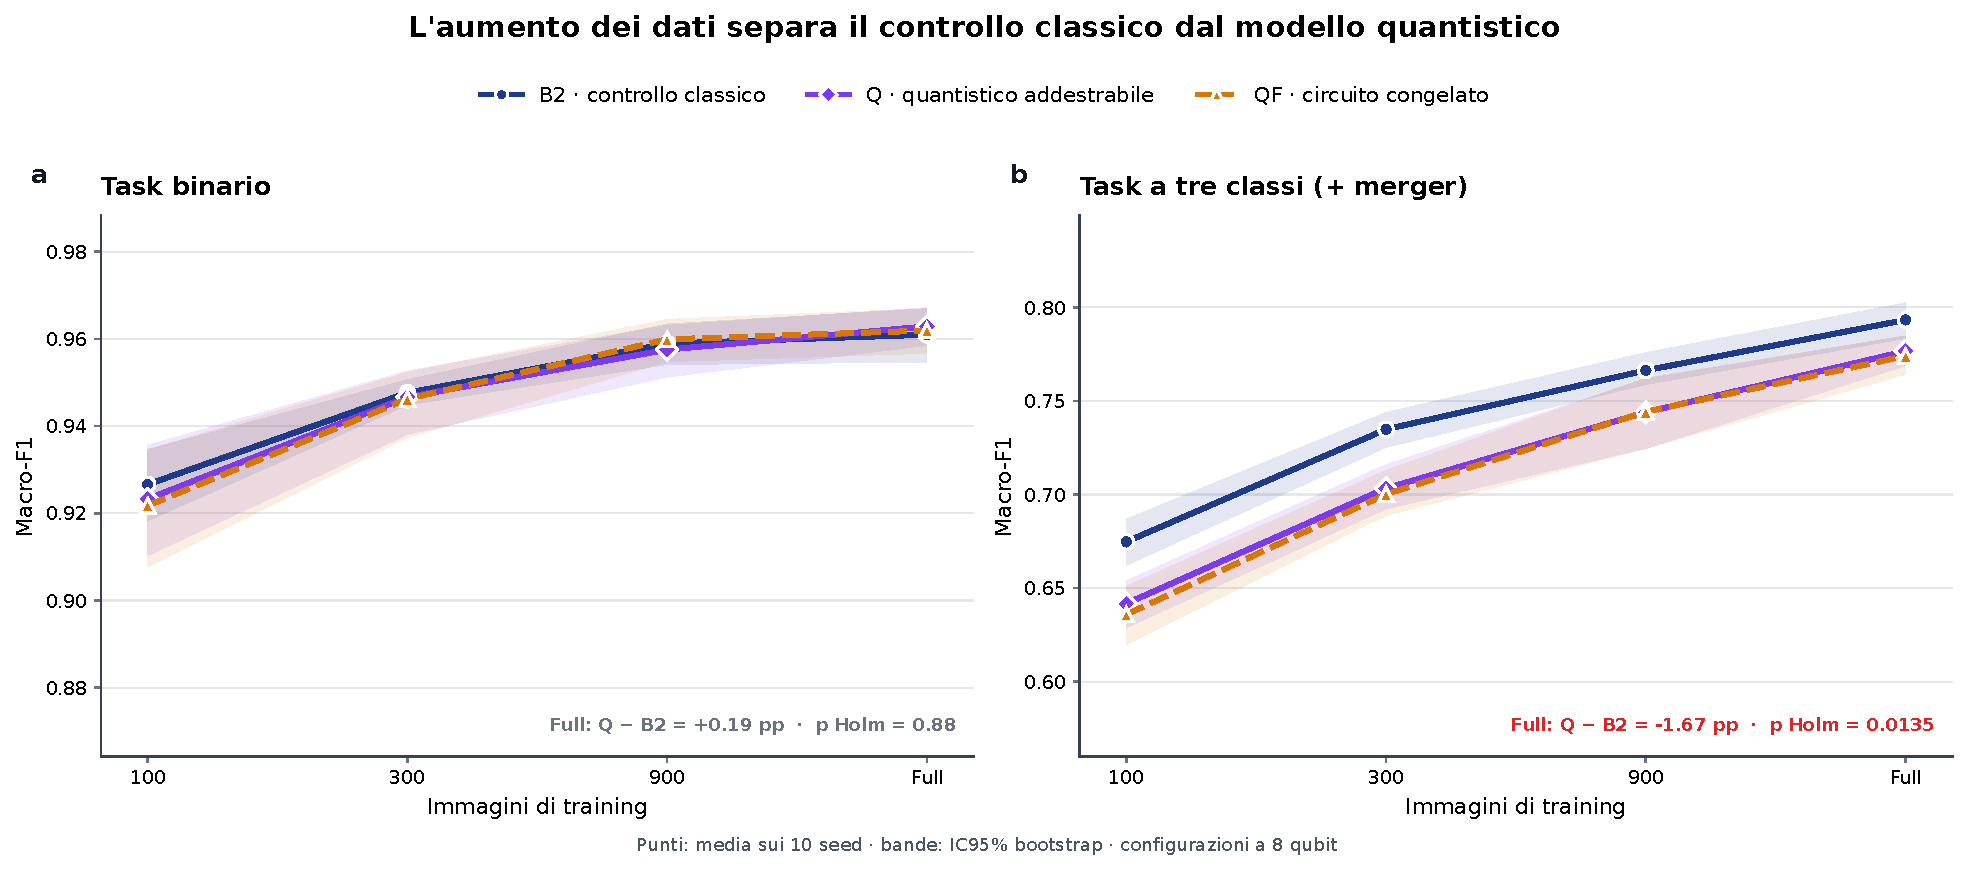
\includegraphics[width=\textwidth,trim=0 0 0 30bp,clip]{01_hero_learning_curves.pdf}
\caption{Prestazioni rispetto alla numerosità del training per B2-8,
Q-8 e QF-8. Punti e linee rappresentano le medie sui dieci seed;
le bande sono IC95\% bootstrap. Le posizioni 100, 300, 900 e Full
sono categoriche ed equidistanti: la pendenza dei segmenti non è
un tasso di miglioramento per immagine. I pannelli adottano scale
verticali diverse; Full contiene 1\,876 immagini nel binario e
2\,814 nel task a tre classi.}
\label{fig:ris-scaling}
\end{figure}

\section{Confronto appaiato Q--B2}
\label{sec:ris-qb2}

\subsection{Famiglia primaria: training completo}

Il confronto primario utilizza, per ogni seed, la differenza tra
la Macro-F1 di Q e quella di B2 con lo stesso task e la stessa
dimensione del bottleneck. Un valore negativo favorisce B2.
La \cref{tab:ris-primari} riporta tutti i quattro confronti Full,
con gli intervalli e i p-value conservati negli artefatti
dell'esperimento.

\begin{table}[htbp]
\centering
\small
\caption{Confronti primari Q--B2 sul Full. Dieci coppie per riga;
Holm è applicato alla famiglia dei quattro test. Gli IC95\% sono
bootstrap marginali. \(d_z\) è la differenza media divisa per la
deviazione standard delle differenze appaiate.}
\label{tab:ris-primari}
\begin{tabular}{lcrrrr}
\toprule
\rowcolor{ThesisTableHeader}
\tablehead{Task} & \tablehead{\(q\)} & \tablehead{\(\Delta\) (pp)} & \tablehead{IC95\% (pp)} & \tablehead{\(p_{\mathrm{Holm}}\)} & \tablehead{\(d_z\)} \\
\midrule
Binario & 4 & \(+0{,}02\) & \([-0{,}29;\,+0{,}33]\) & \(0{,}9406\) & \(+0{,}04\) \\
Binario & 8 & \(+0{,}19\) & \([-0{,}22;\,+0{,}61]\) & \(0{,}8797\) & \(+0{,}27\) \\
Tre classi & 4 & \(-0{,}73\) & \([-1{,}27;\,-0{,}33]\) & \(0{,}0132\) & \(-0{,}87\) \\
Tre classi & 8 & \(-1{,}67\) & \([-2{,}41;\,-1{,}02]\) & \(0{,}0135\) & \(-1{,}40\) \\
\bottomrule
\end{tabular}
\end{table}

Nel binario le differenze medie sono piccole e positive, ma gli
intervalli includono lo zero e nessun p-value corretto è inferiore
a \(0{,}05\). Non emerge quindi evidenza di un vantaggio di Q rispetto
a B2, né la mancanza di significatività consente di dichiararli
equivalenti.

Nel task a tre classi entrambi i confronti indicano invece una
Macro-F1 inferiore per Q, con \(p_{\mathrm{Holm}}<0{,}05\).
La perdita media è di \(0{,}73\) pp a quattro qubit e di
\(1{,}67\) pp a otto qubit. Gli intervalli sono interamente
negativi. La maggiore ampiezza osservata a otto qubit è una
descrizione degli effetti; non costituisce, da sola, un test della
differenza tra i due effetti.

\subsection{Famiglia secondaria: regimi low-resource}

La \cref{tab:ris-secondari} mostra i dodici confronti sui subset.
La correzione di Holm è calcolata su tutte le dodici righe, non
separatamente per task, dimensione o numerosità. Nel binario
nessun confronto risulta significativo dopo questa correzione.
Nel task a tre classi le differenze sono tutte negative; quelle
a otto qubit risultano significative in ciascun subset,
mentre quelle a quattro qubit non raggiungono la significatività.

\begin{table}[htbp]
\centering
\small
\caption{Tutti i confronti secondari Q--B2. Effetti e intervalli
sono espressi in punti percentuali. I p-value sono corretti con
Holm congiuntamente sui dodici confronti.}
\label{tab:ris-secondari}
\begin{tabular}{rlcrrr}
\toprule
\rowcolor{ThesisTableHeader}
\tablehead{Subset} & \tablehead{Task} & \tablehead{\(q\)} & \tablehead{\(\Delta\)} & \tablehead{IC95\%} & \tablehead{\(p_{\mathrm{Holm}}\)} \\
\midrule
100 & Binario & 4 & \(-1{,}61\) & \([-2{,}62;\,-0{,}56]\) & \(0{,}1632\) \\
100 & Binario & 8 & \(-0{,}33\) & \([-1{,}81;\,+0{,}82]\) & \(1{,}0000\) \\
100 & Tre classi & 4 & \(-2{,}88\) & \([-4{,}31;\,-1{,}29]\) & \(0{,}1071\) \\
100 & Tre classi & 8 & \(-3{,}30\) & \([-4{,}99;\,-1{,}80]\) & \(0{,}0396\) \\
\addlinespace
300 & Binario & 4 & \(-0{,}39\) & \([-1{,}42;\,+0{,}58]\) & \(1{,}0000\) \\
300 & Binario & 8 & \(-0{,}10\) & \([-0{,}81;\,+0{,}43]\) & \(1{,}0000\) \\
300 & Tre classi & 4 & \(-2{,}34\) & \([-3{,}76;\,-0{,}83]\) & \(0{,}1632\) \\
300 & Tre classi & 8 & \(-3{,}15\) & \([-4{,}46;\,-1{,}86]\) & \(0{,}0360\) \\
\addlinespace
900 & Binario & 4 & \(+0{,}02\) & \([-0{,}38;\,+0{,}40]\) & \(1{,}0000\) \\
900 & Binario & 8 & \(-0{,}14\) & \([-0{,}44;\,+0{,}11]\) & \(1{,}0000\) \\
900 & Tre classi & 4 & \(-0{,}85\) & \([-1{,}39;\,-0{,}25]\) & \(0{,}1632\) \\
900 & Tre classi & 8 & \(-2{,}24\) & \([-3{,}88;\,-0{,}94]\) & \(0{,}0396\) \\
\bottomrule
\end{tabular}
\end{table}

Con \(100\) immagini, il contrasto binario a quattro qubit è
\(-1{,}61\) pp e il suo IC95\% non include zero, ma il p-value
corretto è \(0{,}1632\). Non è una contraddizione: intervallo
marginale bootstrap e test corretto per la molteplicità non sono
lo stesso criterio decisionale. Lo stesso richiamo vale per i
contrasti a quattro qubit nel task a tre classi.

La \cref{fig:ris-delta} raccoglie i confronti nei quattro regimi.
Non si osserva un vantaggio statisticamente supportato di Q nei
regimi con meno dati. A otto qubit, nel task a tre classi, la
penalità media è anzi più ampia nei subset da \(100\) e \(300\)
immagini rispetto al Full. Si tratta di un andamento descrittivo
tra regimi: i test riportati valutano Q--B2 entro ciascun regime,
non la significatività della sua variazione tra numerosità.

\begin{figure}[htbp]
\centering
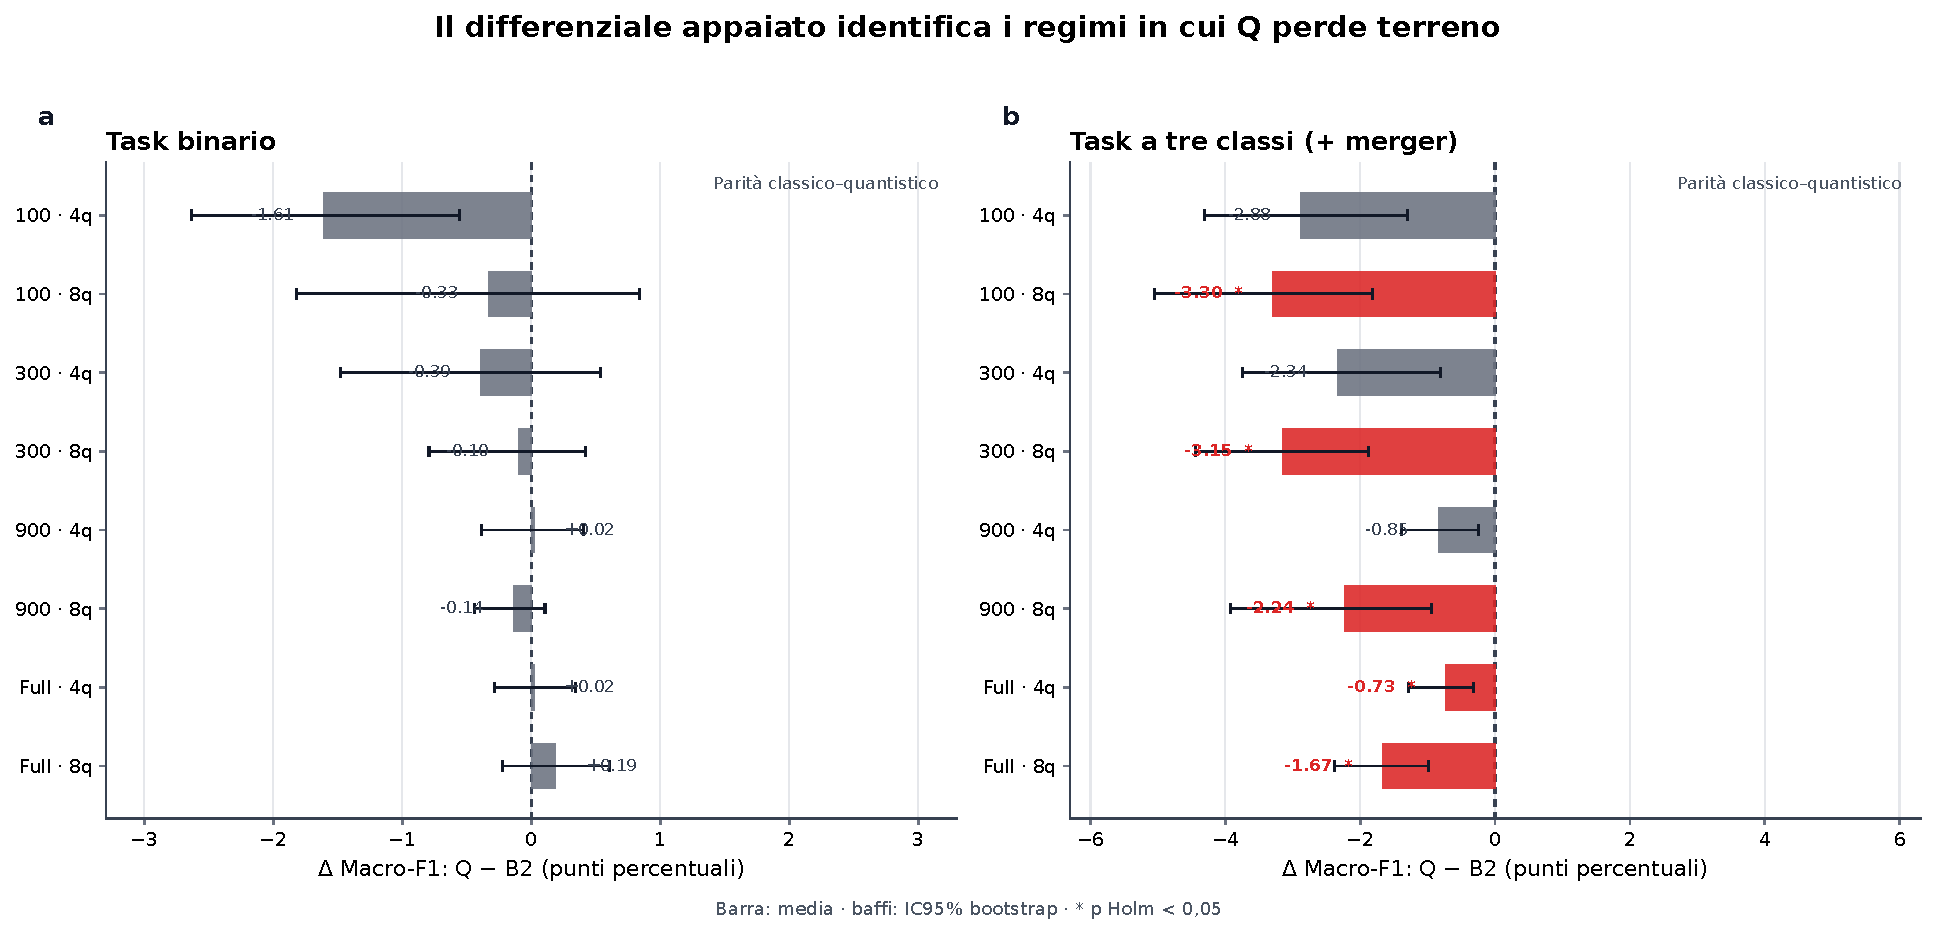
\includegraphics[width=\textwidth,trim=0 0 0 30bp,clip]{02_delta_q_minus_b2.pdf}
\caption{Differenze appaiate Q--B2 nei due task. Barre: differenza
media in pp; baffi: IC95\% bootstrap; asterisco:
\(p_{\mathrm{Holm}}<0{,}05\). I quattro confronti Full e i dodici
sui subset appartengono a famiglie di correzione distinte. Le
scale orizzontali dei pannelli sono diverse. Gli intervalli della
figura sono ricampionati dal notebook grafico e possono differire
lievemente da quelli archiviati nelle
\cref{tab:ris-primari,tab:ris-secondari}.}
\label{fig:ris-delta}
\end{figure}

\section{Passaggio dal binario alle tre classi}
\label{sec:ris-did}

La diminuzione della Macro-F1 assoluta interessa tutti i modelli.
Per isolare sul piano descrittivo la variazione del divario tra Q
e B2, si considera il contrasto
\[
 D_s^{(\mathrm{pp})}=100D_s
 =100\left[(F^{\mathrm Q}_{1,s}-F^{\mathrm{B2}}_{1,s})_{\mathrm{tre}}
 -(F^{\mathrm Q}_{1,s}-F^{\mathrm{B2}}_{1,s})_{\mathrm{binario}}\right].
\]
Qui \(D_s\) è definito nella \cref{eq:did} sulla scala originale
della Macro-F1. Le differenze sono costruite entro lo stesso repeat seed; il
bootstrap ricampiona questi dieci contrasti, non quattro medie
indipendenti. Un valore negativo indica che Q perde terreno
rispetto a B2 nel task a tre classi.

\begin{table}[htbp]
\centering
\small
\caption{Differenza-in-differenze tra task, in pp: media e
IC95\% bootstrap dei contrasti appaiati. Analisi esplorativa,
senza un'ulteriore famiglia di test o correzioni di Holm.}
\label{tab:ris-did}
\begin{tabular}{lrr}
\toprule
\rowcolor{ThesisTableHeader}
\tablehead{Regime} & \tablehead{4 qubit: media [IC95\%]} & \tablehead{8 qubit: media [IC95\%]} \\
\midrule
100 & \(-1{,}27\;[-3{,}13;\,+0{,}86]\) & \(-2{,}97\;[-5{,}17;\,-0{,}78]\) \\
300 & \(-1{,}95\;[-3{,}37;\,-0{,}46]\) & \(-3{,}06\;[-4{,}61;\,-1{,}49]\) \\
900 & \(-0{,}87\;[-1{,}59;\,-0{,}02]\) & \(-2{,}10\;[-3{,}54;\,-0{,}91]\) \\
Full & \(-0{,}75\;[-1{,}42;\,-0{,}24]\) & \(-1{,}86\;[-2{,}56;\,-1{,}21]\) \\
\bottomrule
\end{tabular}
\end{table}

Tutte le stime medie sono negative (\cref{tab:ris-did}). A otto
qubit il contrasto è compreso tra circa \(-3{,}06\) e
\(-1{,}86\) pp e gli intervalli marginali restano sotto lo zero.
A quattro qubit gli effetti sono più contenuti; con \(100\)
immagini l'intervallo attraversa lo zero. Il limite superiore
molto vicino a zero per \(900\) immagini non va interpretato
come una separazione netta tra presenza e assenza dell'effetto.

Questa analisi rende visibile una differenza relativa che sarebbe
poco leggibile rappresentando soltanto il calo comune di circa
venti punti della Macro-F1. Non identifica però un effetto
causale dell'aggiunta della classe merger: cambiano il problema
di classificazione, la composizione dei dati e, sul Full, anche
la numerosità totale del training. La Macro-F1 dei due task è
inoltre una media su un diverso numero di classi.

\section{Analisi della classe merger}
\label{sec:ris-merger}

\subsection{F1, precision e recall}

La classe merger è quella con la F1 media più bassa sul Full
per tutte le configurazioni B2, Q e QF riportate nella
\cref{tab:ris-merger}. Il confronto con le altre due classi
permette di localizzare il divario, senza attribuirgli
automaticamente una causa fisica o un problema nelle etichette.

\begin{table}[htbp]
\centering
\small
\caption{Prestazioni medie per classe sul Full a tre classi,
moltiplicate per 100. Per merger sono riportate anche precision
e recall. Ogni valore è la media della metrica calcolata
separatamente sui dieci test; F1 non è ricostruita dalla
precision e dal recall medi.}
\label{tab:ris-merger}
\begin{tabular}{lrrrrr}
\toprule
& \multicolumn{3}{c}{\tablehead{F1 per classe}} & \multicolumn{2}{c}{\tablehead{Merger}} \\
\cmidrule(lr){2-4}\cmidrule(lr){5-6}
\rowcolor{ThesisTableHeader}
\tablehead{Modello} & \tablehead{Ellittiche} & \tablehead{Spirali} & \tablehead{Merger} & \tablehead{Precision} & \tablehead{Recall} \\
\midrule
\textbf{B2-4} & 84,99 & 81,76 & 70,27 & 72,68 & 68,23 \\
Q-4  & 84,69 & 80,74 & 69,38 & 71,04 & 68,53 \\
QF-4 & 84,70 & 80,49 & 69,17 & 71,59 & 67,59 \\
\addlinespace
\textbf{B2-8} & 85,16 & 82,26 & 70,58 & 73,79 & 67,87 \\
Q-8  & 84,61 & 80,39 & 67,99 & 71,63 & 64,97 \\
QF-8 & 84,83 & 79,66 & 67,73 & 71,53 & 64,90 \\
\bottomrule
\end{tabular}
\end{table}

A otto qubit, Q perde rispetto a B2 circa \(2{,}58\) pp nella
F1 merger, \(1{,}86\) pp nelle spirali e \(0{,}56\) pp nelle
ellittiche. Poiché la Macro-F1 è la media delle tre F1, il
contributo aritmetico della classe merger al divario complessivo
è circa \(2{,}58/3=0{,}86\) pp, poco più della metà dei
\(1{,}67\) pp osservati. Questo è un modo di scomporre la metrica,
non una spiegazione causale degli errori.

A quattro qubit il quadro è meno concentrato sulla merger:
la diminuzione della sua F1 è di \(0{,}88\) pp, mentre per le
spirali è di \(1{,}02\) pp. Inoltre il recall merger di Q-4 è
lievemente superiore a quello di B2-4 (\(68{,}53\) contro
\(68{,}23\)), a fronte di una precision inferiore
(\(71{,}04\) contro \(72{,}68\)). Non sarebbe quindi corretto
descrivere entrambe le dimensioni come un'identica perdita di
capacità di recuperare le merger.

\subsection{Andamento nei subset ed errori di classificazione}

La \cref{fig:ris-merger} mostra che il divario sulla F1 merger
è particolarmente ampio con \(100\) immagini e otto qubit:
Q--B2 è pari a \(-9{,}82\) pp, con IC95\% esplorativo
\([-13{,}32;\,-6{,}72]\). La differenza si riduce a
\(-4{,}82\) pp con \(300\) immagini, \(-3{,}50\) pp con
\(900\) e \(-2{,}58\) pp sul Full. A quattro qubit il divario
medio passa da \(-4{,}47\) pp nel subset minimo a
\(-0{,}88\) pp sul Full, ma non decresce monotonamente:
con \(900\) immagini è di soli \(-0{,}32\) pp.

\begin{figure}[htbp]
\centering
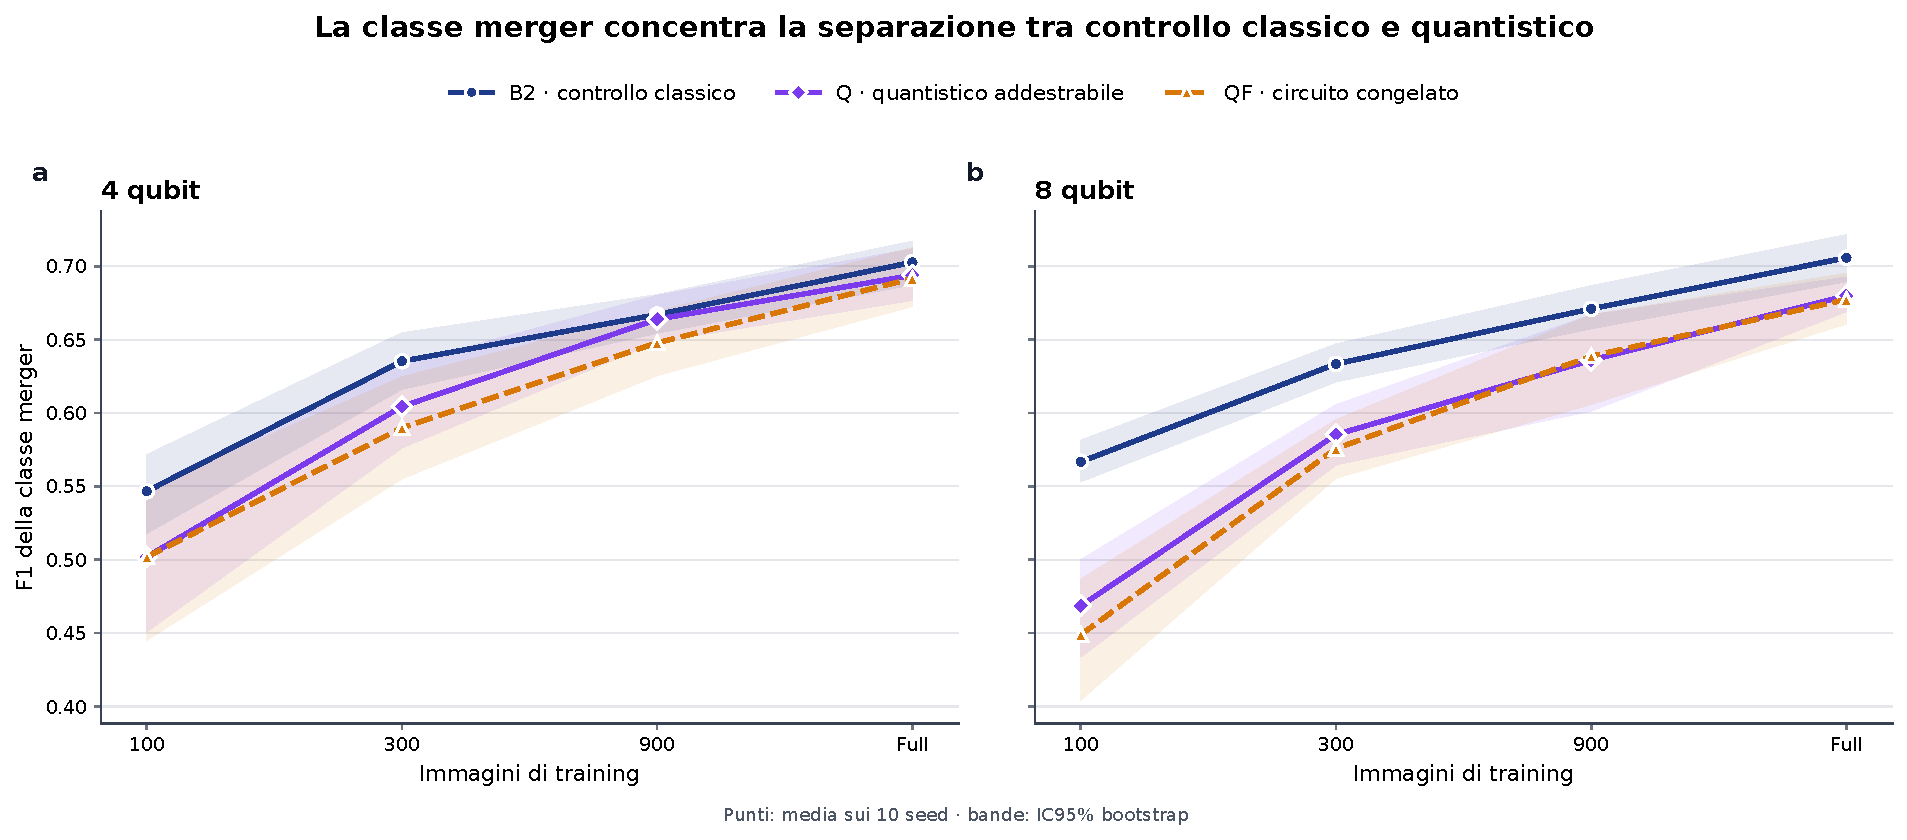
\includegraphics[width=\textwidth,trim=0 0 0 30bp,clip]{04_merger_detailed.pdf}
\caption{F1 della classe merger rispetto al regime di training,
con pannelli separati per quattro e otto dimensioni/qubit.
Le linee rappresentano le medie e le bande gli IC95\% bootstrap.
Le due scale verticali coincidono. La figura descrive la F1 di
una singola classe, non la Macro-F1 dell'intero task.}
\label{fig:ris-merger}
\end{figure}

Le matrici di confusione normalizzate forniscono un riscontro
più specifico sugli errori del Full. Per ogni modello sono state
mediate le matrici normalizzate per riga dei dieci seed, senza
trattare come oggetti distinti le ricomparse di una stessa
galassia in holdout diversi.
In B2-8, in media, il \(17{,}44\%\) delle merger è classificato
come spirale; in Q-8 la quota sale al \(20{,}68\%\).
La quota di merger assegnate alle ellittiche è invece simile:
\(14{,}69\%\) in B2-8 e \(14{,}35\%\) in Q-8.
La diminuzione del recall merger a otto qubit si associa dunque,
in questi tassi medi, soprattutto a più assegnazioni alla classe
spirale.

A quattro qubit, invece, le merger assegnate alle spirali sono
il \(18{,}78\%\) per B2-4 e il \(17{,}91\%\) per Q-4.
Aumenta la confusione nella direzione opposta: le spirali
assegnate alla classe merger passano dal \(13{,}69\%\) al
\(16{,}12\%\). Questo andamento è coerente con la minore
precision merger di Q-4. Le percentuali descrivono tassi medi
per classe vera, non percentuali sull'intero dataset.

\section[Addestramento quantistico e dimensionalità]{Contributo dell'addestramento quantistico e dimensionalità}
\label{sec:ris-ablazioni}

\subsection{Circuito addestrabile rispetto al circuito congelato}

Il confronto Q--QF valuta quanto cambi la prestazione quando i
pesi del circuito vengono ottimizzati, mantenendo addestrabili
le componenti classiche in entrambi i modelli. QF non è quindi
un classificatore interamente congelato.

Sul Full il vantaggio medio di Q è contenuto: nel binario è di
\(0{,}23\) pp a quattro qubit e \(0{,}10\) pp a otto;
nel task a tre classi è di \(0{,}15\) e \(0{,}26\) pp.
Tutti i quattro intervalli bootstrap Full includono lo zero
(\cref{fig:ris-qqf}). Questi dati non documentano un beneficio
netto e uniforme dell'ottimizzazione dei pesi circuitali.

\begin{figure}[htbp]
\centering
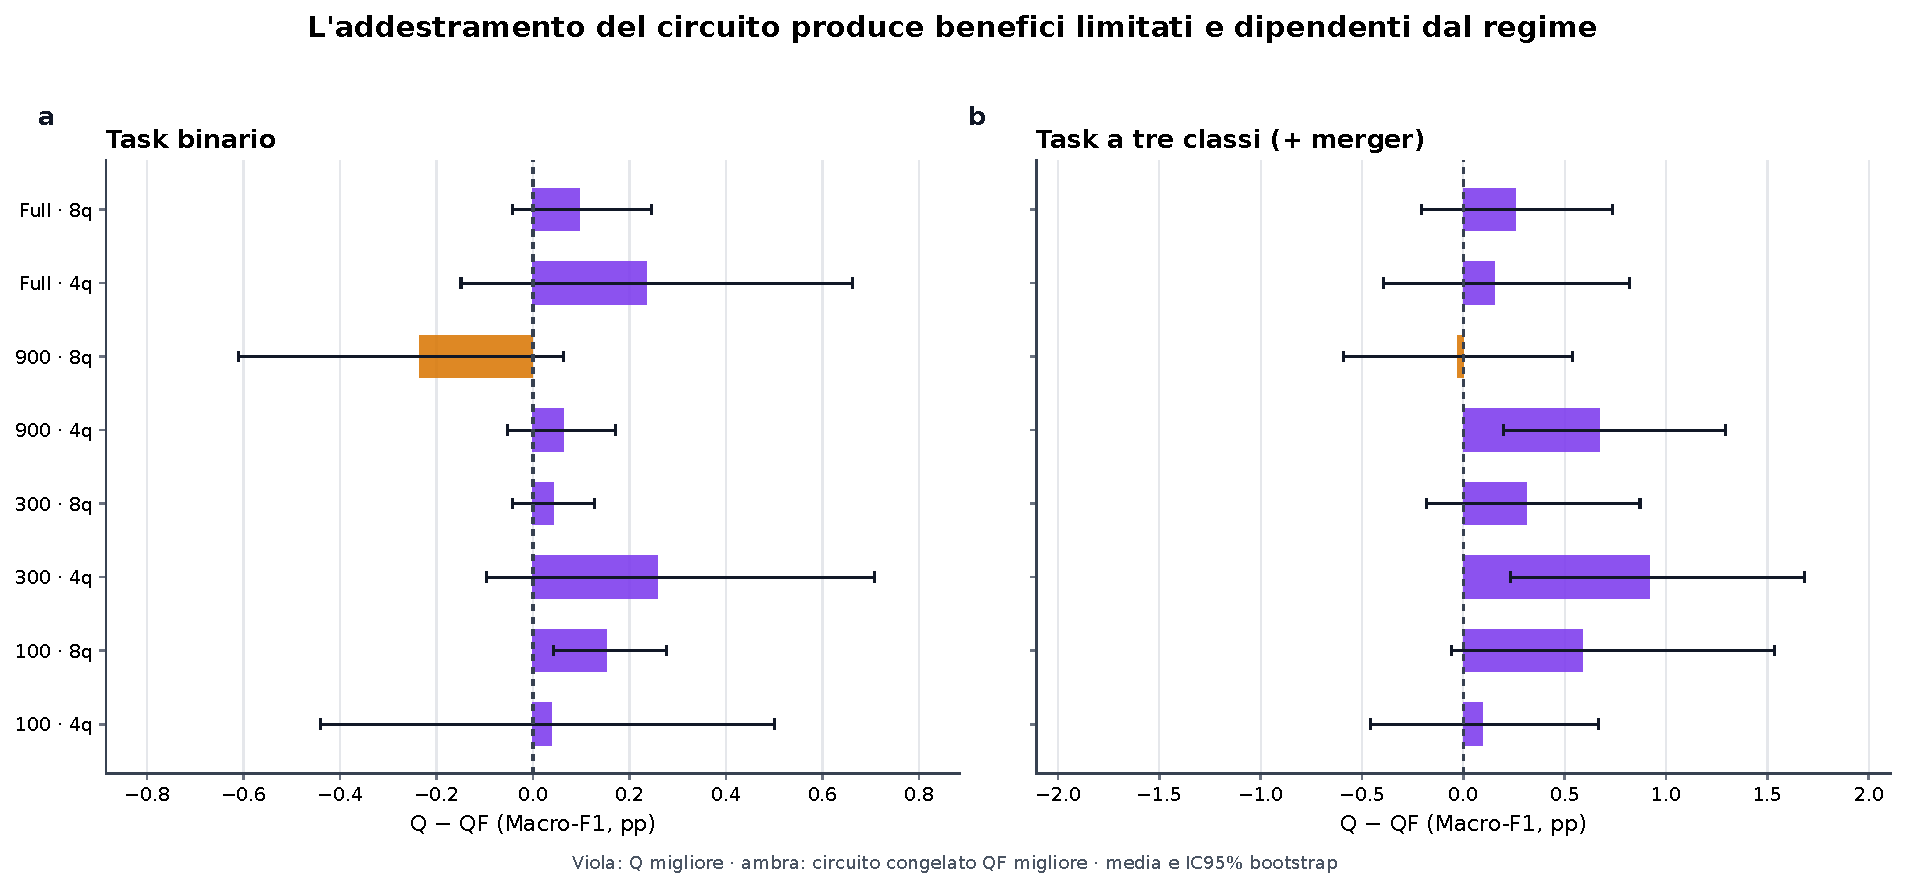
\includegraphics[width=\textwidth,trim=0 0 0 30bp,clip]{05_q_minus_qf.pdf}
\caption{Confronto esplorativo Q--QF: differenza media appaiata
di Macro-F1 in pp e IC95\% bootstrap. Valori positivi favoriscono
Q. I colori indicano il segno dell'effetto, non la significatività.
Le scale orizzontali dei due task sono diverse. Non sono
introdotti nuovi p-value per questi confronti.}
\label{fig:ris-qqf}
\end{figure}

Alcuni subset mostrano effetti più favorevoli a Q. Nel task a
tre classi a quattro qubit, Q--QF è \(+0{,}92\) pp con
\(300\) immagini, con IC95\% circa \([+0{,}24;\,+1{,}70]\),
e \(+0{,}67\) pp con \(900\), con IC95\% circa
\([+0{,}21;\,+1{,}30]\). Nel binario a otto qubit e
\(100\) immagini il vantaggio è più piccolo, \(+0{,}15\) pp,
con IC95\% circa \([+0{,}04;\,+0{,}28]\). Al contrario,
Q-8 nel binario con \(900\) immagini è mediamente inferiore
a QF-8 di \(0{,}24\) pp, con intervallo che include lo zero.
Sono evidenze esplorative e non una nuova serie di risultati
confermativi selezionati in base agli intervalli più favorevoli.

\subsection{Da quattro a otto dimensioni/qubit}

La sensibilità alla dimensione è riassunta nella
\cref{fig:ris-qubit}. Nel binario con \(100\) immagini,
Q-8 supera Q-4 di \(1{,}43\) pp; sul Full la differenza si
riduce a \(0{,}05\) pp. Nel task a tre classi, invece, Q-8
ha una media inferiore a Q-4 in tutti i regimi: le differenze
\(8-4\) sono circa \(-0{,}38\), \(-0{,}69\), \(-1{,}34\)
e \(-0{,}61\) pp per \(100\), \(300\), \(900\) e Full.
Per B2, nello stesso task, le differenze sono piccole e positive.

\begin{figure}[htbp]
\centering
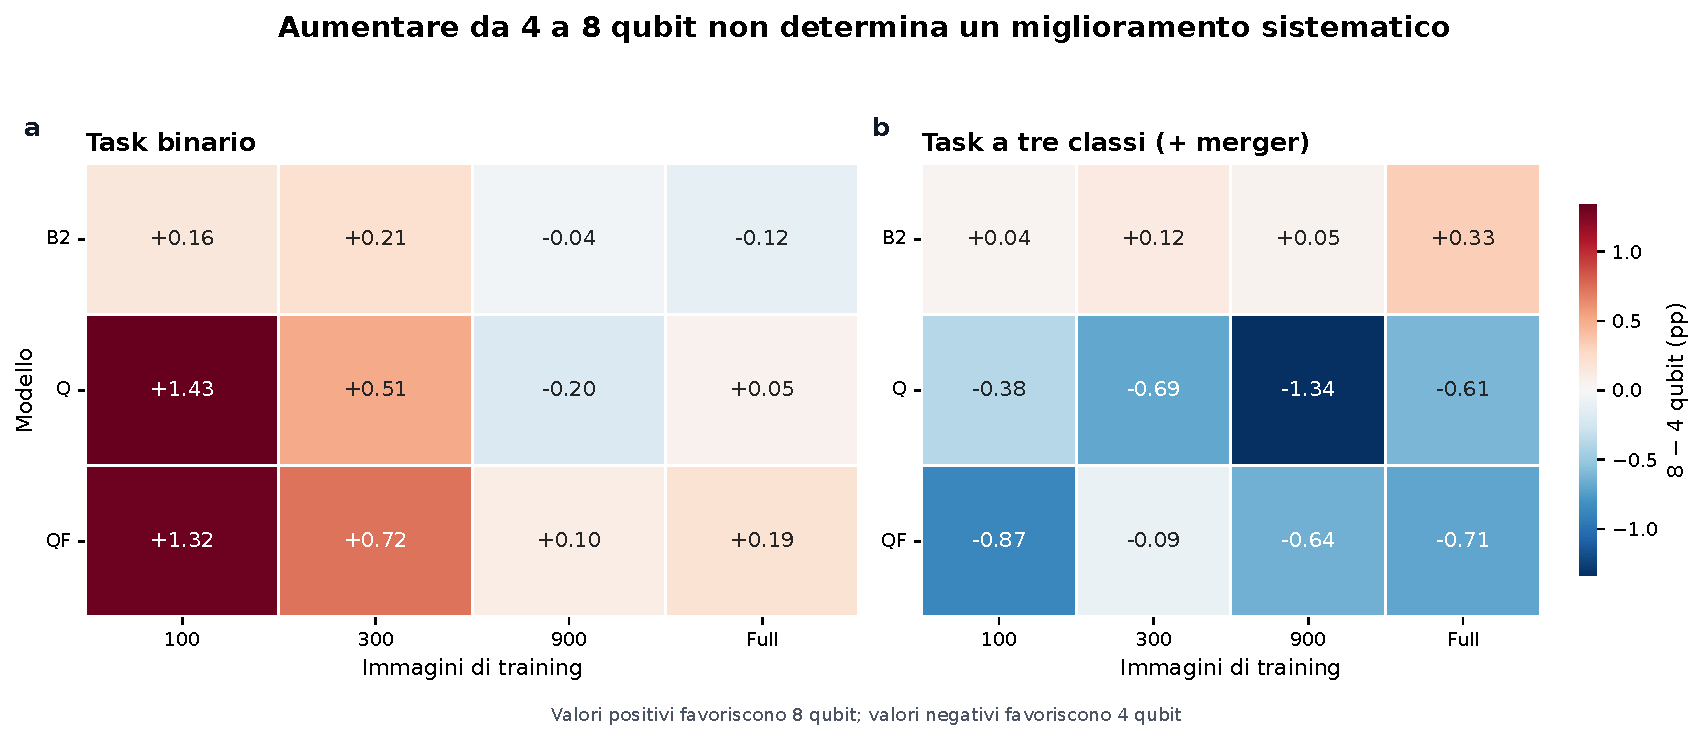
\includegraphics[width=\textwidth,trim=0 0 0 30bp,clip]{06_qubit_sensitivity.pdf}
\caption{Variazione media della Macro-F1 passando da quattro
a otto dimensioni/qubit, in pp. Valori positivi favoriscono
la dimensione otto. La heatmap è una sintesi descrittiva senza
intervalli o marcature di significatività. Per B2 varia la
dimensione del bottleneck classico; per Q e QF cambiano anche
il circuito e le dimensioni dei livelli classici collegati.}
\label{fig:ris-qubit}
\end{figure}

L'aumento della dimensione non coincide dunque con un incremento
sistematico delle prestazioni. Questa osservazione riguarda le
configurazioni effettivamente confrontate: come precisato nel
\cref{chap:modelli}, il passaggio da quattro a otto qubit modifica
anche la proiezione classica e il classificatore finale. Non
isola l'effetto del solo numero di qubit.

\section{Qualità delle probabilità e calibrazione}
\label{sec:ris-calibrazione}

La Macro-F1 valuta le decisioni di classe, ma non esaurisce
l'analisi delle probabilità prodotte dal modello. La
\cref{tab:ris-calibrazione} riporta ECE, Brier score e log-loss
medi sul Full per B2 e Q. Valori più bassi sono preferibili,
ma le tre quantità misurano aspetti diversi; in particolare
Brier score e log-loss non sono misure di sola calibrazione
\cite{gneiting2007scoring}. L'ECE confronta invece accuratezza e
confidenza aggregate in intervalli \cite{guo2017calibration}.

\begin{table}[htbp]
\centering
\small
\caption{Metriche probabilistiche medie sul test Full, senza
ricalibrazione post-hoc. Dieci seed per configurazione. I valori
sono nella scala originale delle metriche, non moltiplicati
per 100. Sintesi descrittiva, senza test aggiuntivi.}
\label{tab:ris-calibrazione}
\begin{tabular}{llrrr}
\toprule
\rowcolor{ThesisTableHeader}
\tablehead{Task} & \tablehead{Modello} & \tablehead{ECE} & \tablehead{Brier score} & \tablehead{Log-loss} \\
\midrule
Binario & B2-4 & 0,0189 & 0,0603 & 0,1205 \\
        & Q-4  & 0,0158 & 0,0610 & 0,1172 \\
        & B2-8 & 0,0205 & 0,0631 & 0,1258 \\
        & Q-8  & 0,0158 & 0,0598 & 0,1160 \\
\addlinespace
Tre classi & B2-4 & 0,0495 & 0,3024 & 0,5137 \\
           & Q-4  & 0,0508 & 0,3132 & 0,5361 \\
           & B2-8 & 0,0570 & 0,2970 & 0,5078 \\
           & Q-8  & 0,0432 & 0,3185 & 0,5417 \\
\bottomrule
\end{tabular}
\end{table}

Nel binario, Q mostra ECE e log-loss medi inferiori a B2 per
entrambe le dimensioni; il Brier score è lievemente superiore
per Q-4 e inferiore per Q-8. Nel task a tre classi, Brier score
e log-loss sono maggiori per Q in entrambe le configurazioni.
L'ECE non segue uniformemente questo ordinamento: Q-8 ha un
ECE medio di \(0{,}0432\), inferiore al \(0{,}0570\) di B2-8,
pur avendo una Macro-F1 inferiore e peggiori Brier score e
log-loss.

Non vi è contraddizione tra questi risultati: una minore
discrepanza media tra confidenza e accuratezza nei bin dell'ECE
non garantisce una migliore discriminazione delle classi o una
migliore qualità probabilistica secondo ogni criterio. Non si
utilizza quindi il solo ECE per ribaltare il confronto sulla
Macro-F1, né un reliability diagram di un singolo seed per
caratterizzare un'intera architettura. I valori assoluti delle
metriche probabilistiche tra binario e tre classi non vanno
letti come se composizione e numero di classi fossero invariati.

\section{Prestazioni e costo computazionale}
\label{sec:ris-costi}

\subsection{Tempi registrati e ambito del confronto}

I tempi sono confrontati tra modelli dello stesso regime, secondo
le condizioni di esecuzione descritte nella \cref{sec:ambiente-hardware}.
Le traiettorie tra regimi hanno funzione descrittiva e non misurano
lo scaling del costo rispetto alla sola numerosità del training.

La \cref{tab:ris-tempi-full} riporta i tempi mediani del Full.
Il tempo di training è la somma dei tempi di epoca registrati:
non include estrazione iniziale delle feature, salvataggio
successivo dei checkpoint, valutazione finale o trasferimenti
degli archivi. Il tempo di predizione qui riportato è invece
lo specifico campo \texttt{test\_inference\_seconds}, riferito
all'intero test dopo il ripristino del checkpoint selezionato.
Non è il campo \texttt{inference\_seconds} delle tabelle
intermedie, che si riferisce alla validation.

\begin{table}[htbp]
\centering
\small
\caption{Tempi mediani sul Full in secondi, sui dieci seed.
Training: somma dei tempi di epoca; test: tempo di predizione
su 938 esempi nel binario e 1\,407 nel task a tre classi.
Le misure escludono la costruzione della cache di feature e
non rappresentano latenze end-to-end delle immagini.}
\label{tab:ris-tempi-full}
\begin{tabular}{lrrrr}
\toprule
& \multicolumn{2}{c}{\tablehead{Binario}} & \multicolumn{2}{c}{\tablehead{Tre classi}} \\
\cmidrule(lr){2-3}\cmidrule(lr){4-5}
\rowcolor{ThesisTableHeader}
\tablehead{Modello} & \tablehead{Training} & \tablehead{Test} & \tablehead{Training} & \tablehead{Test} \\
\midrule
\textbf{B2-4} & 23,88 & 0,192 & 41,90 & 0,287 \\
Q-4  & 250,27 & 2,253 & 441,80 & 3,456 \\
QF-4 & 209,17 & 2,188 & 380,25 & 3,273 \\
\textbf{B2-8} & 23,31 & 0,195 & 42,41 & 0,279 \\
Q-8  & 442,67 & 4,211 & 854,89 & 6,557 \\
QF-8 & 361,37 & 4,181 & 668,88 & 6,692 \\
\bottomrule
\end{tabular}
\end{table}

I tempi di Q sono maggiori di quelli di B2 sia durante il
training sia durante la predizione sul test. QF riduce il
tempo mediano di training rispetto a Q nelle configurazioni
Full, ma resta molto più costoso del controllo classico.
Il congelamento dei pesi circuitali non elimina infatti
l'esecuzione del circuito né la propagazione del gradiente
necessaria ad addestrare la proiezione che lo precede.

\subsection{Rapporti appaiati e compromesso prestazioni--tempo}

La \cref{tab:ris-rapporti} riporta la mediana dei dieci rapporti
\(t_{\mathrm Q,s}/t_{\mathrm{B2},s}\), non il rapporto tra i
tempi mediani della tabella precedente. I rapporti mediani
di training vanno da circa \(10\) a \(15\) a quattro qubit
e da circa \(19\) a \(26\) a otto qubit.

\begin{table}[htbp]
\centering
\small
\caption{Mediana dei rapporti appaiati di tempo di training
Q/B2. Un valore 10 indica un tempo dieci volte quello di B2
secondo questa statistica. Le colonne dei subset provengono
da CPU, la colonna Full da GPU; non sono fattori di scaling
misurati a hardware costante.}
\label{tab:ris-rapporti}
\begin{tabular}{lcrrrr}
\toprule
\rowcolor{ThesisTableHeader}
\tablehead{Task} & \tablehead{\(q\)} & \tablehead{100} & \tablehead{300} & \tablehead{900} & \tablehead{Full} \\
\midrule
Binario & 4 & 14,63 & 11,03 & 10,15 & 10,19 \\
Binario & 8 & 25,66 & 19,10 & 18,97 & 19,26 \\
Tre classi & 4 & 12,18 & 11,14 & 11,11 & 10,58 \\
Tre classi & 8 & 21,44 & 21,56 & 23,95 & 18,58 \\
\bottomrule
\end{tabular}
\end{table}

La \cref{fig:ris-costo} combina Macro-F1 media e tempo di
training mediano. Nel task a tre classi, entro ogni regime,
B2 raggiunge una prestazione media maggiore con un tempo
mediano inferiore rispetto alle corrispondenti configurazioni
Q e QF. Nel binario alcuni punti quantistici hanno una
Macro-F1 media lievemente superiore, ma a fronte di un
costo temporale nettamente maggiore. Non è dunque corretto
descrivere B2 come strettamente dominante in ogni singolo
confronto binario soltanto sulla base del grafico.

\begin{figure}[htbp]
\centering
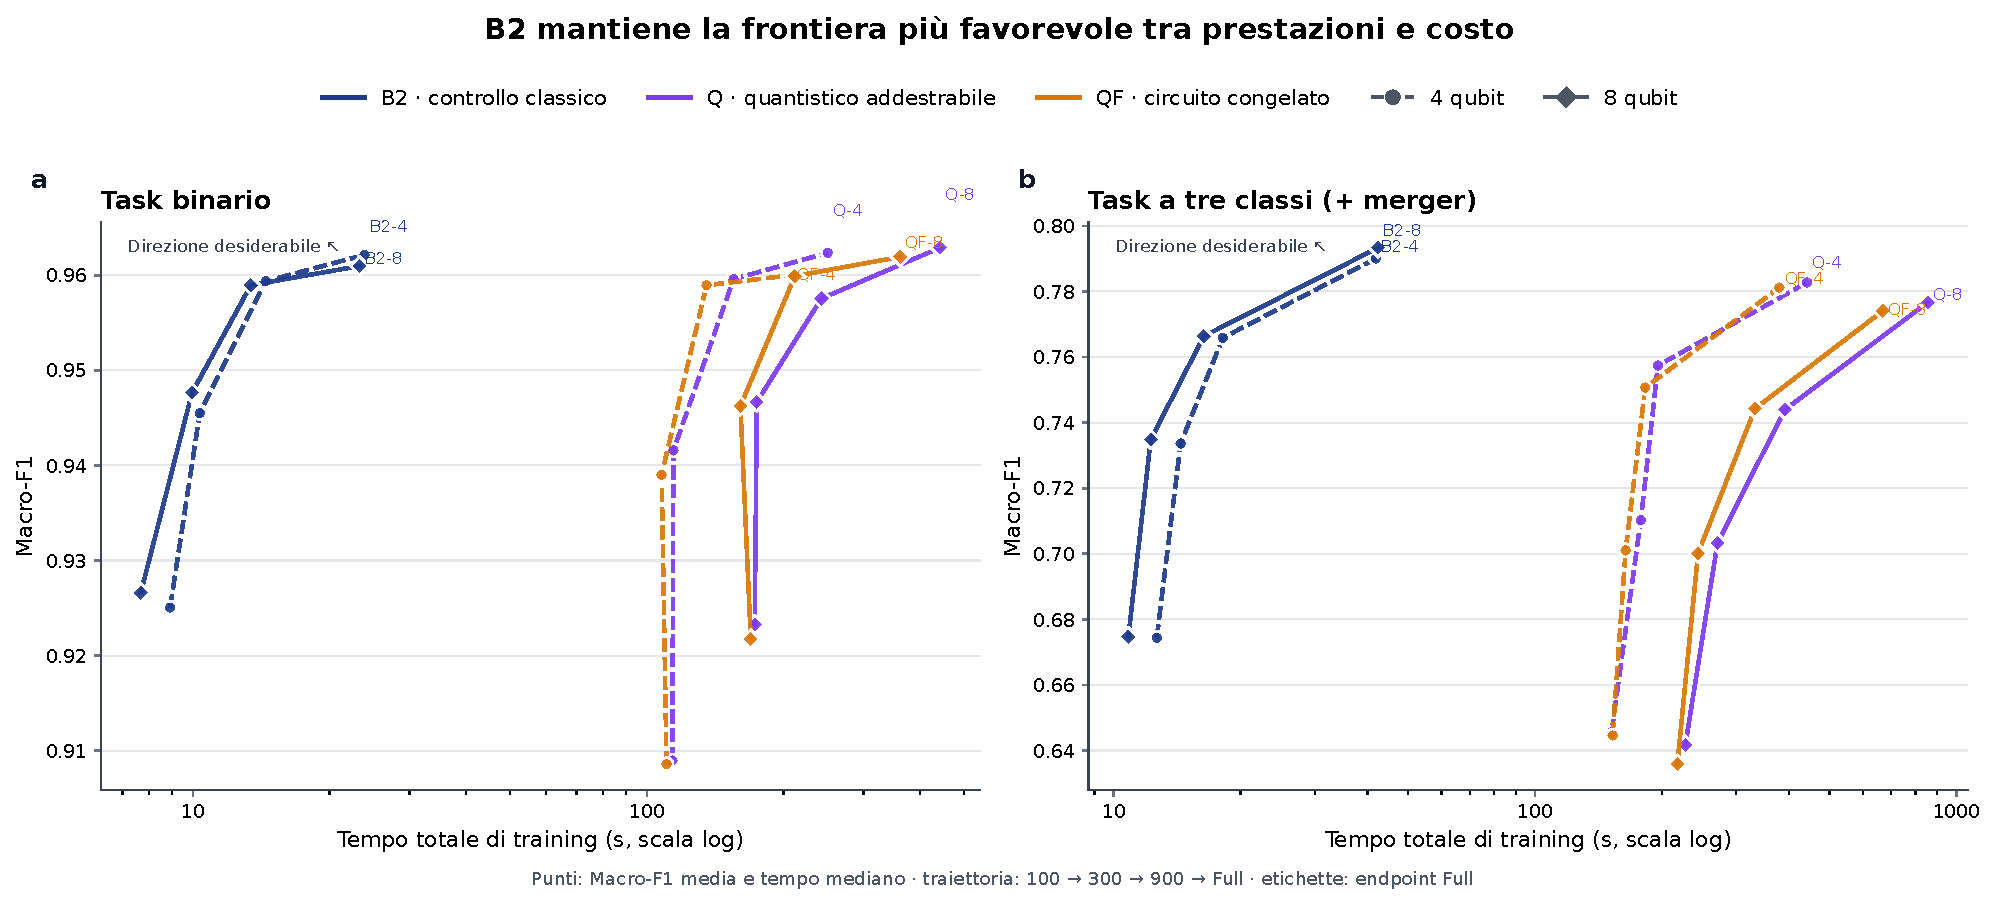
\includegraphics[width=\textwidth,trim=0 0 0 30bp,clip]{07_pareto_performance_cost.pdf}
\caption{Prestazioni e tempo di training osservato: ciascun
punto combina la Macro-F1 media e il tempo mediano delle
dieci run di una configurazione. Le linee collegano, in
ordine, 100, 300, 900 e Full; le etichette identificano
l'estremo Full. L'asse dei tempi è logaritmico. I primi
tre regimi sono eseguiti su CPU, Full su GPU: i segmenti
non definiscono una frontiera a hardware costante né una
legge di scaling. La figura non rappresenta l'incertezza
congiunta di prestazione e tempo.}
\label{fig:ris-costo}
\end{figure}

L'early stopping contribuisce ai tempi complessivi, che
dipendono anche dal numero di epoche effettivamente eseguite.
Le differenze non possono essere attribuite interamente
al costo di una singola valutazione circuitale. Infine,
tutti questi risultati riguardano il simulatore classico
\texttt{default.qubit}: non misurano tempi di una QPU,
costi di accesso all'hardware quantistico o consumi energetici.

\section{Sintesi delle evidenze}
\label{sec:ris-sintesi}

Nel protocollo considerato, le prestazioni medie di tutte le
configurazioni crescono all'aumentare dei dati di training.
Sul Full binario i modelli raggiungono Macro-F1 vicine a
\(0{,}96\), senza evidenza di un vantaggio di Q rispetto
a B2 nei confronti primari. Nel task a tre classi, invece,
Q presenta una Macro-F1 inferiore a B2 per entrambe le
dimensioni, con significatività secondo la procedura
appaiata e la correzione adottate.

Nei regimi low-resource non emerge il vantaggio quantistico
ipotizzato: a otto qubit, nel task a tre classi, le perdite
medie sono maggiori di quelle osservate sul Full e risultano
significative nella famiglia secondaria. L'analisi merger
localizza una parte importante del divario, soprattutto
a otto qubit, senza spiegare da sola tutti gli errori.
Il confronto con QF mostra benefici dell'addestramento
circuitale piccoli sul Full e dipendenti dal regime nei
subset. Aumentare da quattro a otto qubit non offre un
miglioramento sistematico della Macro-F1.

Le metriche probabilistiche aggiungono un quadro non
riducibile al solo ordinamento della Macro-F1; i costi
registrati mostrano invece un aumento consistente del
tempo richiesto dai modelli quantistici simulati rispetto
a B2. Queste evidenze circoscrivono il risultato sperimentale
alle architetture, ai dati e alle condizioni qui analizzati:
non costituiscono un'affermazione generale sull'impossibilità
di un vantaggio del machine learning quantistico.

\chapter{Discussione}
\label{chap:discussione}

Le teste ibride ottengono buone prestazioni sulla rappresentazione
estratta da ResNet18, ma non superano il controllo classico B2 nei
confronti statistici del \cref{chap:risultati}. Per interpretare questo
risultato occorre considerare separatamente la difficoltà del task,
la disponibilità dei dati e il costo. La discussione segue le domande
di ricerca del \cref{sec:intro-rq}; le possibili spiegazioni sono
distinte dai meccanismi effettivamente verificati.

\section{Confronto principale e ruolo della rappresentazione}
\label{sec:disc-rq1}

Per RQ1, i dati non forniscono evidenza di un miglioramento di Q
rispetto a B2. Sul Full binario
le differenze medie sono piccole, pari a \(+0{,}02\) e \(+0{,}19\)
punti percentuali per quattro e otto qubit, senza significatività
dopo Holm. Sul Full a tre classi si osservano invece differenze di
\(-0{,}73\) e \(-1{,}67\) pp, significative secondo la procedura
adottata. L'assenza di significatività nel primo caso non dimostra
equivalenza, che richiederebbe un margine definito e un test dedicato.

Le buone prestazioni di B0 e B1 aiutano a interpretare questo quadro.
Una parte rilevante dell'informazione discriminativa è già contenuta
nelle feature classiche. La componente quantistica non deve apprendere
una rappresentazione direttamente dai pixel, ma rielaborare una
rappresentazione preesistente dopo una forte compressione. La domanda
non riguarda pertanto la superiorità di un intero sistema di visione
quantistico, bensì il valore aggiunto di una particolare testa.

B2 conserva prestazioni competitive con un bottleneck di sole quattro
o otto componenti. Ciò indica che, nelle condizioni osservate, la
compressione non impedisce di ottenere buoni risultati. Non dimostra
che le altre componenti delle feature siano sempre inutili, né che
qualsiasi proiezione verso poche dimensioni sarebbe sufficiente:
la proiezione è addestrata insieme al classificatore.

Nel binario il livello prossimo a \(0{,}96\) di Macro-F1 è compatibile
con una situazione in cui il margine di miglioramento misurabile è
contenuto. L'espressione effetto soffitto va tuttavia intesa come
interpretazione: non sono noti l'errore irriducibile del problema o
il massimo conseguibile con le etichette disponibili. La convergenza
delle medie non basta a identificarli.

\section{Complessità del task e classe merger}
\label{sec:disc-rq2}

La risposta a RQ2 è che il divario relativo diventa più sfavorevole
a Q nel passaggio alle tre classi. La differenza-in-differenze sul
Full è di circa \(-0{,}75\) pp a quattro qubit e \(-1{,}86\) pp
a otto. Questo contrasto è più informativo del solo calo assoluto
di Macro-F1, che interessa tutti i modelli.

Non si tratta però di un effetto causale isolato dell'aggiunta dei
merger. Cambiano il numero di classi, la composizione degli esempi
e, sul Full, la numerosità del training. Inoltre, la Macro-F1
media due oppure tre F1 per classe. La conclusione sostenibile è
quindi una variazione osservata del confronto relativo tra task,
non la quantificazione di una penalità fisica attribuibile a una
sola categoria.

I sistemi etichettati come merger costituiscono un banco di prova utile:
formano la classe con F1 media più bassa sul Full per B2, Q e QF. A otto qubit,
il loro contributo aritmetico rappresenta poco più della metà dello
scarto complessivo Q--B2 nella Macro-F1. Le matrici di confusione
mostrano anche più merger assegnate alle spirali da Q-8. A quattro
qubit, invece, il quadro include una perdita di precision merger
con recall lievemente superiore al controllo. Non esiste quindi
un'unica modalità di errore comune alle due configurazioni.

La maggiore eterogeneità visuale dei sistemi perturbati è una
spiegazione plausibile della difficoltà condivisa dai modelli.
I risultati non permettono però di distinguere quanto dipenda dalla
rappresentazione congelata, dalla testa, dall'ambiguità delle etichette
o dalle condizioni osservative. Attribuire gli errori direttamente
all'incapacità del circuito di riconoscere specifiche strutture
astronomiche richiederebbe esperimenti ulteriori.

\section{Disponibilità dei dati e regimi low-resource}
\label{sec:disc-rq3}

RQ3 verifica se il circuito sia particolarmente utile quando il
training contiene pochi esempi. Le evidenze non sostengono questa
ipotesi nel protocollo considerato. Nelle tre classi Q ha una media
inferiore a B2 in tutti i regimi; a otto qubit le differenze dei
tre subset rimangono significative dopo la correzione secondaria.
Il divario medio passa da \(-3{,}30\) pp con 100 immagini a
\(-1{,}67\) pp sul Full: cresce la prestazione di entrambi e lo
scarto si riduce, senza annullarsi.

Questo andamento mostra perché sia utile non limitarsi al training
completo. Le prestazioni vicine sul task binario non descrivono
l'intero comportamento delle architetture; task più articolati e
subset ridotti possono rendere visibili differenze attenuate altrove.
La F1 merger con 100 immagini e otto qubit, inferiore in Q di circa
\(9{,}82\) pp rispetto a B2, rappresenta uno di questi casi,
da interpretare come analisi esplorativa di una singola classe.

La selezione dei subset dal medesimo training mantiene controllata
la provenienza dei dati, senza dimostrare l'annidamento reciproco
dei campioni ridotti. Le variazioni possono quindi riflettere anche
la composizione dei campioni. Inoltre, con batch e limite di epoche
fissati, un dataset più piccolo produce meno aggiornamenti per epoca;
l'early stopping modifica inoltre la durata effettiva. Le curve
descrivono quindi il comportamento del protocollo a differenti
numerosità, non un esperimento a identico numero di aggiornamenti.

\section{Addestramento circuitale e numero di qubit}
\label{sec:disc-rq4}

Il confronto Q--QF risponde alla prima parte di RQ4. Sul Full i
vantaggi medi di Q sono compresi tra circa \(0{,}10\) e \(0{,}26\)
pp e tutti gli intervalli includono lo zero. Non emerge dunque un
beneficio netto e uniforme dell'ottimizzazione circuitale, pur in
presenza di alcuni effetti esplorativi più favorevoli nei subset.

La vicinanza tra Q e QF è compatibile con un ruolo importante degli
strati classici che precedono e seguono il circuito. QF può adattare
gli angoli di ingresso attraverso la proiezione e modificare la
decisione finale attraverso il classificatore: non è un modello
privo di apprendimento. Non si può quindi dedurre che il circuito
sia ignorato, che i suoi gradienti siano nulli o che la rete sia
equivalente a un classificatore lineare.

La seconda parte di RQ4 riguarda la dimensionalità. Otto qubit non
offrono un miglioramento sistematico: nel task a tre classi Q-8
ha una media inferiore a Q-4 in tutti i regimi, mentre nel binario
con 100 esempi l'ordinamento è opposto. Più qubit non costituiscono
quindi, in queste configurazioni, una garanzia di maggiore utilità
predittiva.

Il passaggio da quattro a otto modifica però anche proiezione,
classificatore, numero di rotazioni e collegamenti circuitali.
Il confronto non identifica l'effetto separato di ciascun elemento.
Una maggiore difficoltà di ottimizzazione o una diversa adeguatezza
della trasformazione ai dati sono ipotesi possibili, non meccanismi
dimostrati dal solo ordinamento delle medie.

In particolare, non viene diagnosticato un barren plateau. Il fenomeno
descritto da McClean et al.~\cite{mcclean2018barren} richiede condizioni
e misure specifiche. Come chiarito nel metodo, il campo diagnostico
denominato \texttt{quantum\_gradient\_norm} include anche parametri
classici e non permette di isolare i gradienti degli angoli variazionali.
Né la loro scomparsa né la loro adeguata ampiezza possono essere
concluse da quella diagnostica aggregata.

\section{Qualità probabilistica e costo computazionale}
\label{sec:disc-rq5}

Le metriche probabilistiche aggiungono informazioni che la Macro-F1
non contiene. Un modello può avere decisioni meno accurate e una
confidenza mediamente più coerente con la propria frequenza di successo.
Questo aiuta a leggere il caso di Q-8 sulle tre classi: l'ECE medio
è inferiore a quello di B2-8, ma Brier score e log-loss sono peggiori.
Non è una contraddizione e non costituisce un ribaltamento del
confronto predittivo. Le metriche valutano aspetti diversi e l'ECE
dipende anche dal binning \cite{guo2017calibration,gneiting2007scoring}.

Per RQ5 il costo osservato è nettamente sfavorevole ai modelli
quantistici simulati. Sul Full, le mediane dei rapporti appaiati
di training Q/B2 sono circa dieci a quattro qubit e diciannove a
otto. Nelle tre classi B2 combina inoltre una Macro-F1 media
superiore con tempi mediani inferiori. Nel binario i piccoli
vantaggi medi di alcune configurazioni Q non sono statisticamente
supportati e richiedono comunque un costo maggiore.

QF riduce il costo di training rispetto a Q sul Full, ma resta
più costoso di B2. Congelare il circuito non evita la sua esecuzione
né la differenziazione rispetto agli ingressi necessaria per
addestrare la proiezione. La distinzione tra pesi congelati e
assenza di calcolo del gradiente è quindi rilevante anche dal
punto di vista computazionale.

I tempi riguardano le teste simulate ed escludono l'estrazione delle
feature. Il diverso ambiente di esecuzione tra regimi
(\cref{sec:ambiente-hardware}) e il numero di epoche determinato
dall'early stopping impediscono di attribuire tutte le variazioni
temporali alla numerosità dei dati o al costo delle porte.
Queste misure non consentono inoltre di stimare tempi o consumi di una QPU.

\section{Relazione con la letteratura}

Il lavoro conferma la praticabilità dello schema di transfer learning
ibrido introdotto da Mari et al.~\cite{mari2020transfer}: la
rappresentazione classica consente di utilizzare piccoli circuiti
su immagini di dimensione elevata. Questa fattibilità è distinta
dalla superiorità predittiva. Anche l'interesse per piccoli dataset
documentato nel telerilevamento \cite{otgonbaatar2023transfer} motiva
una verifica, ma non implica che lo stesso comportamento debba
emergere sulle galassie.

I risultati sono coerenti con l'esigenza metodologica evidenziata
da Bowles et al.~\cite{bowles2024benchmarking}: la scelta di
baseline e condizioni sperimentali influenza ciò che si può
attribuire alla componente quantistica. Qui B2 è particolarmente
informativo perché conserva il bottleneck e gli strati classici
di interfaccia senza inserire il circuito.

Questa coerenza non rende equivalenti gli esperimenti. Dataset,
encoding, ansatz, ottimizzatori e criteri di selezione differiscono
tra gli studi. Il contributo della tesi è un'evidenza documentata
su un preciso problema applicativo, non una confutazione generale
delle possibilità del quantum machine learning.

\section{Limiti e minacce alla validità}
\label{sec:disc-limiti}

\subsection{Campione, etichette e generalizzazione esterna}

Il dataset è un campione selezionato e bilanciato, non una rappresentazione
delle frequenze morfologiche di una survey completa. Le soglie sui voti
definiscono classi operative e possono privilegiare esempi con maggiore
accordo. Le metriche ottenute non determinano quindi direttamente
le prestazioni su popolazioni con prevalenze, qualità osservative o
livelli di ambiguità diversi.

Le partizioni separano gli identificativi degli oggetti, ma non sono
costruite raggruppando sistemi fisici o regioni di cielo. L'unicità
degli identificativi non garantisce l'indipendenza astronomica di
tutti gli esempi. Una validazione esterna e controlli sulle eventuali
correlazioni spaziali rafforzerebbero la valutazione della generalizzazione.

\subsection{Rappresentazione, iperparametri e ambito architetturale}

Il backbone congelato rende il confronto più controllato, ma limita tutte le teste
all'informazione disponibile nelle feature estratte. Non viene studiato
se il fine-tuning sul dominio galattico cambi il confronto Q--B2.
I risultati riguardano angle encoding singolo, profondità due e
quattro oppure otto qubit; non includono altre famiglie di circuiti,
rumore fisico o misure a shot finiti.

Gli iperparametri fissati favoriscono la comparabilità ma non equivalgono
a una ricerca esaustiva del migliore assetto per ogni architettura.
Una configurazione condivisa può essere più adatta a un modello
che a un altro. B0 e B1 usano inoltre batch diversi dal confronto
principale: le loro prestazioni offrono contesto, non isolano
esclusivamente l'effetto della forma della testa.

\subsection{Ripetizioni e inferenza statistica}

Le dieci ripetizioni condividono il dataset e possono includere
gli stessi oggetti in test differenti. Non sono dieci campioni
astronomici indipendenti. Il bootstrap sui seed e il test sign-flip
non modellano esplicitamente questa dipendenza, mentre la correzione
di Holm tratta la molteplicità e non corregge le assunzioni dei test
di partenza. Le cautele discusse da Nadeau e Bengio
\cite{nadeau2003inference} restano quindi pertinenti.

L'appaiamento riduce la confusione dovuta a confronti su split
diversi, ma non elimina questi limiti. Intervalli, p-value e
dimensioni dell'effetto devono essere letti insieme, distinguendo
evidenze primarie e osservazioni esplorative. Il numero complessivo
di 640 run non va scambiato per 640 repliche indipendenti di
ciascun confronto: ogni contrasto utilizza dieci coppie.

\subsection{Audit, casi particolari e interpretabilità}

La conservazione di predizioni, checkpoint e cronologie consente
di controllare la coerenza degli aggregati e di esaminare casi
particolari. Un seed favorevole o un'immagine classificata
correttamente soltanto da Q può suggerire un'analisi, ma non
sostituisce il confronto aggregato e non giustifica l'esclusione
di run meno favorevoli.

Analogamente, una mappa di attribuzione visuale evidenzia contributi
locali alla risposta del modello secondo il metodo utilizzato,
non una spiegazione causale completa della decisione. Le analisi
qualitative devono essere accompagnate da criteri espliciti di
selezione degli esempi e non usate per trasformare un caso
illustrativo in una proprietà generale dell'architettura.

\section{Sintesi interpretativa}

Il quadro osservato distingue la capacità di classificare dall'utilità
di introdurre il circuito. Le teste ibride raggiungono prestazioni
elevate sul binario, ma il controllo classico ottiene risultati
vicini con costi inferiori. Nelle tre classi e soprattutto in
alcuni regimi ridotti il divario diventa più sfavorevole a Q.
L'addestramento circuitale e l'aumento dei qubit non offrono
benefici uniformi.

Per le configurazioni studiate, il costo aggiuntivo non è accompagnato
da un vantaggio predittivo dimostrato. Una prosecuzione motivata del
lavoro è verificare quali trasformazioni siano adatte alle feature
disponibili e quanto l'ottimizzazione riesca a sfruttarle, prima di
aumentare ulteriormente la complessità del circuito. È una direzione
di ricerca suggerita dagli esperimenti, non una conclusione generale
sull'utilità del quantum machine learning.

\chapter{Conclusioni e sviluppi futuri}
\label{chap:conclusioni}

\section{Sintesi del lavoro}

In questo lavoro ho confrontato teste classiche e ibride
classico-quantistiche per la classificazione morfologica delle galassie.
Il dataset bilanciato di \(5\,628\) immagini ha permesso di definire due task e di
esaminare il ruolo della disponibilità dei dati attraverso subset
stratificati del training. La matrice finale comprende \(640\) run,
organizzate su dieci ripetizioni di holdout stratificato.

La rappresentazione condivisa di ResNet18 ha consentito di
concentrare l'analisi sulle teste. Le baseline B0 e B1 hanno
fornito riferimenti classici; B2 ha controllato la compressione
a quattro o otto componenti; Q e QF hanno distinto l'inserimento
del circuito dall'addestramento dei suoi parametri. Prestazioni,
incertezza, errori per classe e tempi sono stati esaminati
congiuntamente.

Sul Full binario le architetture raggiungono Macro-F1 prossime
a \(0{,}96\), senza evidenza di un vantaggio di Q rispetto a B2.
Sul Full a tre classi Q presenta invece una perdita media di
\(0{,}73\) pp a quattro qubit e \(1{,}67\) pp a otto,
significativa secondo i test e la correzione adottati. I regimi
con pochi dati non mostrano il beneficio quantistico ipotizzato;
l'analisi merger rende visibile una parte importante delle
difficoltà, soprattutto a otto qubit.

Il contributo dell'addestramento circuitale risulta contenuto
sul Full e dipendente dal regime nei subset. L'aumento dei qubit
non determina miglioramenti sistematici. I tempi dei modelli
quantistici simulati sono invece sensibilmente maggiori di quelli
del controllo classico.
Le conclusioni restano circoscritte a dataset, rappresentazione,
circuiti e protocollo considerati.

\section{Contributi e valore del confronto}

Il risultato del lavoro è un confronto riproducibile su dati
astronomici. Immagini, partizioni, configurazioni e predizioni
rimangono collegate negli artefatti, consentendo di risalire
dalle metriche aggregate alle singole esecuzioni.

La combinazione di controlli classici, circuito congelato e
regimi di dati rende il risultato più informativo di una sola
misura di accuratezza. Permette di distinguere ciò che il modello
ibrido riesce a fare da ciò che apporta rispetto alle alternative.
Nelle condizioni esaminate, il circuito non offre un miglioramento
predittivo che compensi il maggiore costo osservato.

Il protocollo costituisce inoltre una base riutilizzabile per
valutare modifiche successive. Nuove rappresentazioni o circuiti
possono essere confrontati mantenendo criteri espliciti di
appaiamento e una distinzione tra analisi confermative ed
esplorative.

\section{Sviluppi futuri}
\label{sec:concl-futuro}

\subsection{Validazione esterna e robustezza del protocollo}

La priorità è verificare la generalizzazione su un campione
indipendente, possibilmente con condizioni osservative o
prevalenze diverse. Partizioni per regione di cielo o sistema
fisico aiuterebbero a controllare correlazioni non eliminate
dalla sola separazione degli identificativi. Analisi di
sensibilità alle soglie di etichettatura potrebbero inoltre
chiarire quanto il confronto dipenda dalla selezione di
esempi più o meno ambigui.

Sul piano statistico, ulteriori valutazioni dovrebbero
considerare esplicitamente la dipendenza tra split e definire
in anticipo famiglie di confronti e differenze di interesse
pratico. Se l'obiettivo fosse dimostrare che due modelli
hanno prestazioni sufficientemente vicine, servirebbe un
protocollo di equivalenza o non inferiorità, non la sola
assenza di significatività.

\subsection{Rappresentazione e ottimizzazione}

Una seconda direzione riguarda l'adeguatezza delle feature
al dominio galattico. Backbone preaddestrati su immagini
astronomiche o un fine-tuning controllato potrebbero cambiare
la qualità della rappresentazione disponibile alle teste.
Ogni modifica dovrebbe essere applicata anche ai controlli
classici per non attribuire al circuito un beneficio dovuto
all'estrattore.

È inoltre utile confrontare strategie di ottimizzazione con
budget di ricerca espliciti e comparabili, distinguendo
numero di epoche, aggiornamenti e tempo disponibile. Questo
permetterebbe di verificare se gli iperparametri condivisi
abbiano favorito alcune teste e se una diversa ottimizzazione
cambi il divario osservato.

\subsection{Ablazioni circuitali e diagnostiche mirate}

Le modifiche al circuito dovrebbero rispondere a ipotesi
specifiche: cambiare profondità, collegamenti o encoding
separatamente è più informativo che aumentare simultaneamente
tutte le componenti. Il data re-uploading, non usato nel
circuito principale, rappresenta una possibile estensione
da confrontare con controlli classici adeguati.

Per comprendere il ruolo dell'addestramento quantistico
occorrerebbe registrare separatamente gradienti e variazioni
dei soli parametri circuitali. Esperimenti con circuito
senza entangling gate e analisi della sensibilità agli
ingressi potrebbero verificare quale parte della trasformazione
sia effettivamente utile. Si tratterebbe di nuovi esperimenti,
non di spiegazioni già dimostrate dai risultati disponibili.

\subsection{Costo e condizioni di esecuzione realistiche}

Un benchmark su hardware costante, con misure end-to-end
e separazione tra estrazione delle feature, training e
inferenza, renderebbe più completa l'analisi dei costi.
L'introduzione di shot finiti e rumore consentirebbe poi
di studiare la sensibilità delle predizioni a condizioni
più vicine all'esecuzione fisica.

Un'eventuale sperimentazione su QPU richiederebbe di misurare
anche preparazione, compilazione, numero di valutazioni e
costi di accesso, evitando di trasferire direttamente i
tempi del simulatore all'hardware quantistico. Il criterio
resterebbe il beneficio ottenuto rispetto a risorse e
prestazioni dei controlli classici.

\section{Considerazione conclusiva}

Gli esperimenti mostrano che piccoli circuiti quantistici possono
essere integrati nella pipeline e raggiungere buone prestazioni,
ma che questo non basta a renderli preferibili al controllo classico.
Con le feature e le condizioni adottate, B2 offre un compromesso
più favorevole tra prestazioni e tempo. Il risultato riguarda le
architetture valutate e non esclude benefici in altri contesti.
Gli sviluppi successivi dovranno verificare quali modifiche alla
rappresentazione, al circuito o all'ottimizzazione cambino questo
confronto, mantenendo controlli e criteri di valutazione espliciti.

\appendix
\chapter{Query di estrazione del catalogo}
\label{app:query}

La query seguente documenta la selezione iniziale effettuata tramite
CasJobs. I nomi delle colonne esportate coincidono con quelli utilizzati
dalla pipeline locale. Il vincolo di etichetta univoca descritto nella
\cref{sec:etichette} viene applicato dopo l'esportazione.

\begin{minted}{sql}
SELECT
    p.objid,
    p.ra,
    p.dec,
    z.p_el_debiased AS prob_elliptical,
    z.p_cs_debiased AS prob_spiral,
    z.p_mg AS prob_merger,
    s.z AS redshift
INTO mydb.GalaxyCandidates_Final
FROM PhotoObj AS p
JOIN zooSpec AS z ON p.objid = z.objid
JOIN SpecObj AS s ON p.objid = s.bestObjID
WHERE
    p.clean = 1
    AND p.type = 3
    AND p.g BETWEEN 14 AND 17.5
    AND s.z BETWEEN 0.005 AND 0.1
    AND (
        z.p_el_debiased > 0.8
        OR z.p_cs_debiased > 0.8
        OR z.p_mg > 0.4
    )
\end{minted}

Il CSV locale non conserva \texttt{clean}, \texttt{type} e \(g\).
La verifica retrospettiva di questi vincoli richiede pertanto
l'accesso al catalogo sorgente, non il solo manifest finale.

\chapter{Codice del confronto appaiato}
\label{app:codice-appaiamento}

I frammenti seguenti provengono da \texttt{paired\_model\_comparison}
nel modulo \texttt{evaluation/statistics.py}. Sono estratti, non
programmi autonomi: import e controlli preliminari sono omessi e i
ritorni a capo sono adattati alla pagina. Il chiamante filtra prima
task e numero di qubit e passa Q come \texttt{model\_a}, B2 come
\texttt{model\_b}. Il confronto primario riguarda il solo Full;
i confronti secondari sono separati per numerosità.

\begin{code}
\begin{minted}{python}
pairing_keys = [
    key for key in (seed_column, "fold", "repeat", "subset_size")
    if key in frame.columns
]
selected = frame.loc[
    frame["model"].isin([model_a, model_b]),
    pairing_keys + ["model", metric]
]
if selected.duplicated(pairing_keys + ["model"]).any():
    raise ValueError("Esistono più risultati per la stessa coppia modello/fold/seed")
paired = selected.pivot(
    index=pairing_keys, columns="model", values=metric
).dropna()
\end{minted}
\caption{Costruzione delle coppie e rifiuto delle osservazioni duplicate.}
\label{lst:paired-code}
\end{code}

Il nome tecnico \texttt{fold} è conservato negli artefatti, ma nella
matrice analizzata vale sempre 1: non indica l'esecuzione di una
cross-validation completa. La funzione verifica inoltre che esistano
coppie complete prima di procedere. Nel \cref{lst:paired-bootstrap}
le differenze sono raggruppate per seed; ciascun contrasto della tesi
comprende dieci unità di ricampionamento, non 640 osservazioni.

\begin{code}
\begin{minted}{python}
paired_differences = (
    (paired[model_a] - paired[model_b])
    .rename("difference").reset_index()
)
inference_values = (
    paired_differences.groupby(seed_column, sort=True)["difference"]
    .mean().to_numpy(dtype=np.float64)
)
rng = np.random.default_rng(seed)
bootstrap_indices = rng.integers(
    0, len(inference_values),
    size=(n_bootstrap, len(inference_values))
)
bootstrap_means = inference_values[bootstrap_indices].mean(axis=1)
confidence_interval = np.quantile(bootstrap_means, [0.025, 0.975])
\end{minted}
\caption{Bootstrap percentile sulla media delle differenze appaiate.}
\label{lst:paired-bootstrap}
\end{code}

Il ricampionamento conserva l'appaiamento Q--B2, ma non corregge
la dipendenza tra holdout sovrapposti. Valgono quindi le limitazioni
discusse nei capitoli metodologico e di discussione. I p-value e la
correzione di Holm costituiscono passaggi distinti da questi intervalli.


\bibliographystyle{plain}
\bibliography{Bibliography}
% Ringraziamenti facoltativi: attivare dopo averli compilati.
% \thispagestyle{plain}
\textbf{There will be the thanks to precious people here.}

\lipsum[1-3]

\end{document}
% -----------------------------------------------------------------
